% !TeX spellcheck = en_US
% Paperformat
% https://tex.stackexchange.com/questions/428553/add-bibliography-as-part-instead-of-chapter-in-toc
\documentclass[a4paper, 12pt, bibliography=totoc]{scrartcl}
%\usepackage{cite}
\usepackage{ragged2e}
\usepackage{url}
\usepackage{bm} % bold math
\usepackage{nccmath} % medium fraction with mfrac 
\usepackage{amssymb}
\usepackage{enumitem}
\usepackage{graphicx}
\usepackage{amsthm} % theorems
\usepackage{hyperref}
\usepackage{float}
\usepackage{listings} % code
\usepackage{xcolor}
\usepackage{longtable} % breaks pages
\usepackage{tabularx}
\usepackage{thmtools}
\usepackage{booktabs}
\usepackage[framemethod=TikZ]{mdframed}
\usepackage[export]{adjustbox}

\declaretheoremstyle[
headfont=\bfseries,
notefont=\bfseries,
%notebraces={(}{)},
qed=,
headpunct=.,
headformat={\mbox{\NAME{} \NUMBER}}
%headformat={\mbox{\NAME{} \NUMBER\NOTE}}
]{custom}

\declaretheoremstyle[
headfont=\bfseries, 
notebraces={[}{]},
bodyfont=\normalfont,
headpunct={},
postheadspace=\newline,
spacebelow=\parsep,
spaceabove=\parsep,
mdframed={
	backgroundcolor=blue!10, 
	innertopmargin=6pt,
	roundcorner=10pt, 
	innerbottommargin=6pt, 
	skipabove=\parsep, 
	skipbelow=\parsep } 
]{thmstyle}

\declaretheorem[style=thmstyle, name=Theorem]{thm}
\declaretheorem[style=custom, name=Example]{example}
\declaretheorem[name=Method call]{mycall}

\usepackage[style=alphabetic,backend=biber]{biblatex}
\addbibresource{bibtex.bib}

\definecolor{light-gray}{gray}{0.9}
\lstset{tabsize=2, linewidth=1.05\textwidth, framextopmargin=1em, basicstyle=\small\ttfamily}
\lstset{numbers=left,backgroundcolor=\color{light-gray}}
\newtheorem{theorem}{Theorem}[section]
\setlength{\textheight}{1.05\textheight}
\newcolumntype{Y}{>{\centering\arraybackslash}X}

\begin{document}
\def\myauthor{Martin Röbke} 
\def\mycoauthor{Dr. Johannes Fichte} 
\def\mytitle{Visualizing Dynamic Programming on Tree Decompositions} 
\def\mydate{\today} 
\def\mymatriculation{3949819}
\def\mybirthday{04.03.1995}
\def\myemail{Martin.Roebke@tu-dresden.de}

\begin{titlepage}
	\vspace*{\stretch{1}}
	\begin{center}
		\textsc{\large 
		{Technische Universität Dresden \\
			Fakultät Informatik} \\
		[8ex]}             
		{\Large\bfseries Bachelor Thesis}           \\[12ex]
		
		{\huge\bfseries \mytitle}                  \\[6.5ex]
		
		\vspace{12ex}
			
		
		{\Large 
		\begin{tabular}{p{0.47\textwidth}l}
		
			\textit{Author:}&  \textit{Supervisor:}\\
			
			\myauthor &  Dr. Johannes Fichte\\
			
			& \textit{Second Supervisor:}\\
			&  Prof. Dr. Stefan Gumhold\\[20ex]
		
		\end{tabular}
		}
		
		
		\vfill
		\textsc{International Center For Computational Logic 		\\[4ex]}
		\mydate
	\end{center}
	\vspace{\stretch{2}}
\end{titlepage}
\newpage
%==============================================================================
%============== DECLARATION ===================================================
%==============================================================================
\section*{ }
\thispagestyle{empty}
{\huge\bfseries{Erklärung zur Urheberschaft}\vspace{20pt}}

\noindent
Hiermit versichere ich, dass diese Arbeit von mir persönlich verfasst ist und dass ich
keinerlei fremde Hilfe in Anspruch genommen habe. Ebenso versichere ich, dass diese Arbeit
oder Teile daraus weder von mir selbst noch von anderen als Leistungsnachweis oder als Leistung, die als Prüfungsvoraussetzung
zu erbringen war, andernorts bereits eingereicht wurden. Wörtliche oder sinngemäße Übernahmen aus anderen Schriften
oder Veröffentlichungen in gedruckter oder elektronischer Form sind gekennzeichnet.
Sämtliche Sekundärliteratur und sonstige Quellen sind nachgewiesen und in der Bibliographie aufgeführt.
Das Gleiche gilt für graphische Darstellungen und Bilder sowie für alle Internet-Quellen. \\[20pt]

\noindent
\myauthor \\\\
Geburtsdatum \mybirthday\\
Matrikelnummer \mymatriculation\\\\
E-Mail-Adresse:\\
 \myemail\\[80pt]


Dresden,  ............................. \hfill .............................
\begin{flushright}
	(Unterschrift)\hspace{1em}
\end{flushright}


\newpage

%==============================================================================
%============== ABSTRACT ======================================================
%==============================================================================
\section*{Abstract}
\vspace{4ex}

Answering questions that can be expressed using graph theory is increasingly interesting in scientific work.
Many problems like Boolean satisfiability or traffic related problems can be translated into connections and nodes.
We think that the use of graph structures can help to further develop algorithms in different areas.

The algorithms we visualize in this thesis use dynamic programming on tree decompositions of graphs.
We preprocess the input graph into a customized tree-decomposition of small tree-width.
This gives us a description of the processing sequence for the algorithm, and allows 
with right hindsight for good parallelization while keeping the solving times competitive even on on larger instances.

Since the design of dynamic programming can be quite error-prone, a fast and uncomplicated visualization is needed for the solution process.

To help further refine and visualize the dynamic programming,
we specified a JSON template for communication between solvers and the newly created visualization tool \href{https://github.com/VaeterchenFrost/tdvisu}{TDVisu}.

As two reference implementations of dynamic programming on tree decompositions we selected the existing solvers \href{https://github.com/daajoe/GPUSAT}{GPUSAT} and \href{https://github.com/hmarkus/dp_on_dbs}{dpdb}.\\


As a side note: \\
Of course the information we visualize is mostly in the solver and could be read out as text. But as the saying goes: ``a picture is worth a 100 spreadsheets".


%  table
{\setlength{\textheight}{1.02\textheight}\newpage
	
\tableofcontents
}

% chapter on next page
\newpage

%==============================================================================
%============== INTRODUCTION ==================================================
%==============================================================================

\section{Introduction}
\subsection{Motivation}

The goal of this thesis is to improve the progress in developing dynamic programming solutions on tree decomposition through visualization.

Graph-algorithms and problems regarding graph-related data are increasingly interesting in scientific work, as the applications of interconnected datasets grow. One interesting paper about graphs in (natural) language processing is \cite{jones-etal-2013-modeling}.
Some use cases include fields of interest like cited in \cite{graphUseCases}: % (see also \url{neo4j.com/use-cases})
\begin{itemize}
	\item[-] Network and Database Infrastructure
	\item[-] Recommendation Engines
	\item[-] Artificial Intelligence and Analytics
\end{itemize}

As illustrations of the possibilities for an application, smaller examples from the problem types Boolean satisfiability \textbf{SAT}, model counting SAT \textbf{\#SAT} and \textbf{minimal vertex cover} are presented.
We also show an example of finding  and visualizing a faulty tree-decomposition that occurred during development.


The target audience for this work includes: 
\begin{itemize}
	\item Developers of dynamic programming on tree decompositions for debugging,
	\item Researchers of such algorithms for comparisons and visualizations,
	\item Teachers and students looking for automatic visualization of their problem instances and the solving process.
\end{itemize} 

%The idea for this project comes from my supervisor Dr. Johannes Fichte, who works with many projects such as \href{https://github.com/hmarkus/dp_on_dbs}{dpdb} on solving monadic second order logic (MSOL) problems using highly parallelized architectures like graphics processing units or state of the art databases.
%One early implementation is published in \cite{evaluationMSO} where for different real world examples the results looked promising
%These projects are very competitive ????REF????? for solving even large instances of those problems.

%============== Concept ====================================================
\subsection{Research Question}
When developing techniques for dynamic programming for various problems or platforms there can be errors in actual implementations that will be hard to pin down. 

There is some evidence and experience in e.g. \cite{SoftwareVisualization, ELVIZ} that visualization of intermediate and final results can help to understand various issues - such as correctness and efficiency of the algorithms.

As there was no tailored tool for our use case yet, it should be created and integrated into existing tools with a minimum of additional effort.

So our main research questions we want to answer with this thesis are:
\begin{enumerate}
	\item How could a prototype visualization and debugging tool for solvers of MSO logic problems using dynamic programming on tree decompositions look like?
	\item How could an implementation of visualization in existing solvers look like?
\end{enumerate}
\noindent
To answer these questions we have implemented TDVisu, a visualization software based on \href{https://graphviz.org/}{Graphviz}. 
Our proposed solution is inspired by previous manual visualizations like the two examples in Figure \ref{fig:prevvisus}.
\begin{figure}[h]
	
	\centering
	\begin{tabularx}{\textwidth}{ X X }
		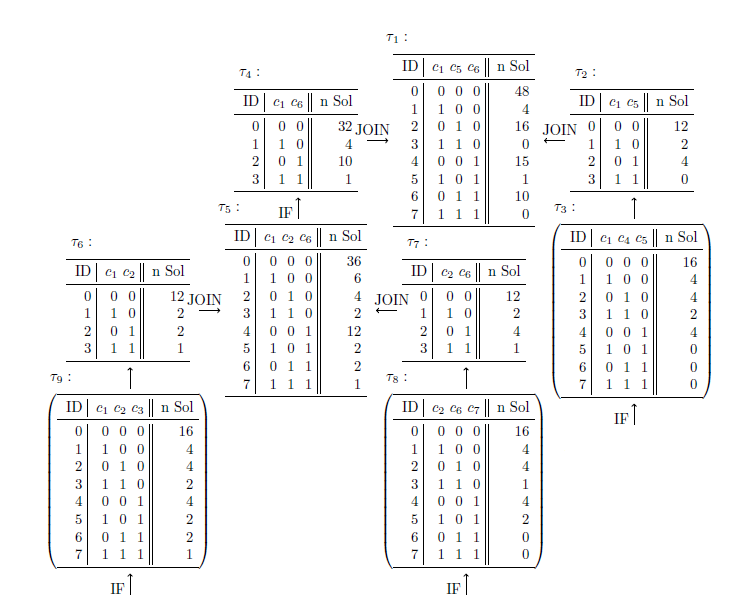
\includegraphics[width=1.05\linewidth,valign=c]{images/DualDA43.png} &  
		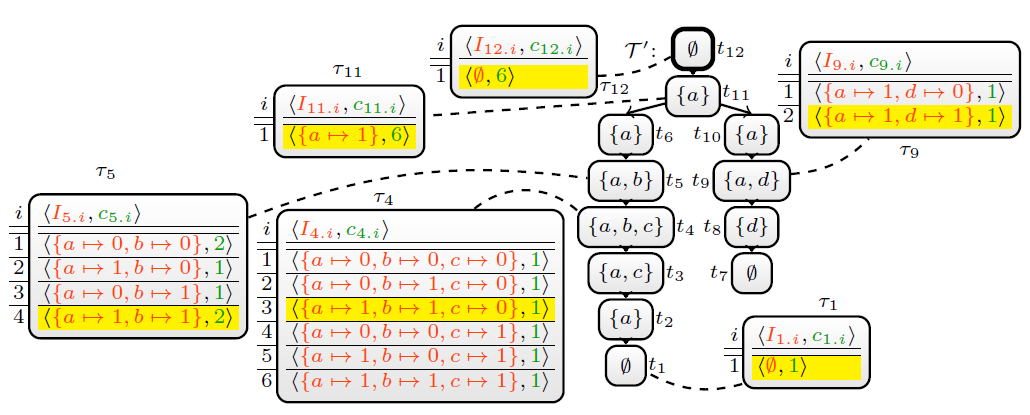
\includegraphics[width=1.02\linewidth,valign=c]{images/dpdbVisuSat.png}\\ 
		
	\end{tabularx}	
	
	\caption{Two templates from published project documentations which show similar visualizations as TDVisu. The left graphic from \cite{DiplomarbeitZisser} Figure 4.3 on page 29 and the right graphic from \cite{dpdbpadl2020} Figure 2, page 4.}
	\label{fig:prevvisus}
\end{figure}

The Figure \ref{fig:overviewprog} shows a draft of the process creating the visualization with TDVisu.

\begin{figure}
	\centering
		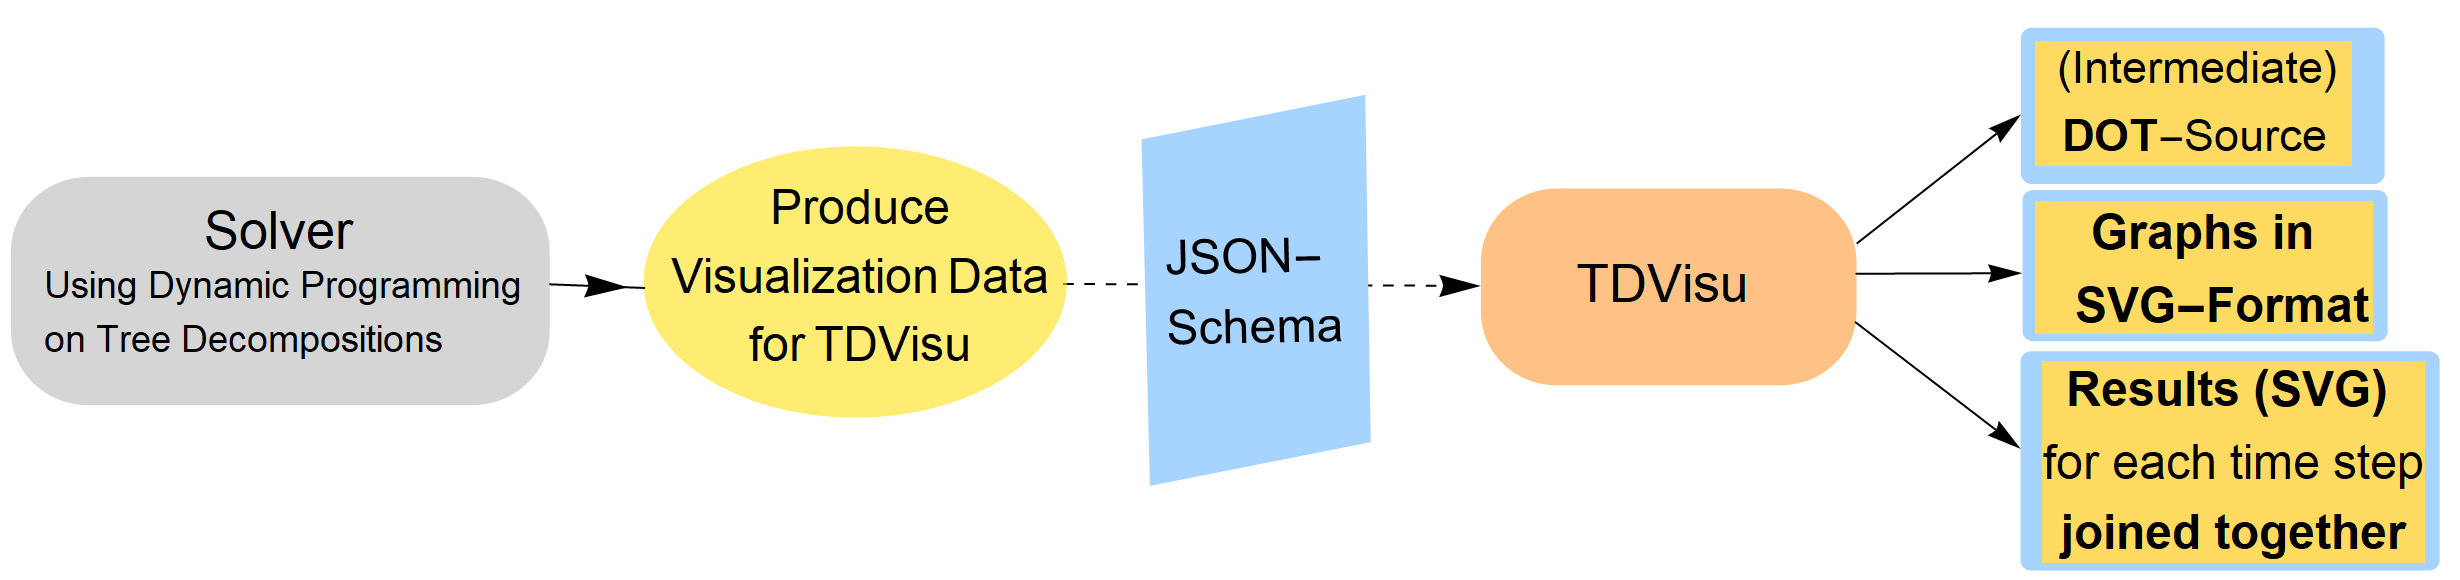
\includegraphics[width=1\linewidth]{images/OverviewProgram.png}
		
	\caption{An overview of the intended use of the visualization. Starting with a solver for DP on TD, over the extraction of the desired data, labels and parameters to the result files.}
	\label{fig:overviewprog}
\end{figure}


%============== Outline ====================================================
\subsection{Methodology}

The algorithms whose runs we visualize basically work so that the input graph is used to find the best possible processing sequence adapted to the hardware.
With this order it is known which parts of the problem can be solved separately, and which intermediate results have to be stored and for how long. To visualize these algorithms for different problem types, we need to be flexible enough with the data we process for visualization. To accomplish this, we almost everywhere expect simple text to be included in various places. Only the internal ids for nodes or variables in Boolean formulas are processed based on positive integers.

For our visualizations we chose {Graphviz}\footnote{\url{https://graphviz.org/}} as an open source graph visualization software, which offers customizable visualization for directed and undirected graphs.

The source code for TDVisu is available under the GPL3 license on \url{github.com/VaeterchenFrost/tdvisu}. The tool is written in python and published on pypi.\\

We defined a \href{https://www.json.org/json-en.html}{JSON}-format specification for portability and customization of the visualization in one file and two reference implementations in practical solvers.\\
It is explained in more detail in the implementation chapter, or directly in the \textit{tdvisu/TDVisu.schema.json} file, a JSON-schema \footnote{\url{http://json-schema.org/draft-07/schema}} with examples and an almost complete validation of the format.

The implementation currently does not support hyper-graphs and assumes that each node in the tree decomposition has either one or two children.
The visualization output consists by default of scalable-vector-graphics (SVG), a very flexible text-based standard for describing images that can be easily compressed (and modified) without loss of quality \cite{SVGMozilla}.

The tree decompositions in every tested application were provided by the utility \href{https://github.com/mabseher/htd}{htd} (small but efficient C++ library for computing (customized) tree and hypertree decompositions) \cite{htd}.


%My previous experiences with the topic of this work mainly come from these two courses:
%\begin{itemize}
%	\item ``Computational Physics" - visualizing with python and matplotlib, by Prof. Dr. A. Bäcker,
%	chair of computational physics, TU Dresden 2016
%	\item ``Graph Data Management and Analytics" - algorithms and various manipulations on graphs, by Hannes Voigt in 2019. \cite{VLGDMA}
%\end{itemize}

%============== Rel Work ====================================================
\subsection{Related Work}

To the best of our knowledge no comparable tool exists that is capable of out-of-the-box visualization of dynamic programming on tree decompositions.
In this chapter, however, we would like to mention works that deal with the surroundings of our problem.

First two papers dealing with additional solvers exploiting small tree-width and Courcelle's Theorem:
\begin{itemize}
	\item ``Implementing Courcelle's Theorem in a declarative framework for dynamic programming" in \cite{ImplCourcelleDP16} \\
	and
	\item ``Evaluation of an MSO-solver" from \cite{evaluationMSO}
\end{itemize}
%Many computationally hard problems become tractable if the graph structure underlying the problem instance exhibits small treewidth. A recent approach to put this idea into practice is based on a declarative interface to Answer Set Programming that allows us to specify dynamic programming over tree decompositions in this language, delegating the computation to dedicated solvers. In this article, we prove that this method can be applied to any problem whose fixed-parameter tractability follows from Courcelle's Theorem. \cite{ImplCourcelleDP16}
%% Journal of Logic and Computation, Volume 27, Issue 4, June 2017, Pages 1067–1094, https://doi.org/10.1093/logcom/exv089
%%Published:
%%07 January 2016
%
%A fundamental theorem of Courcelle states that every problem definable in Monadic Second-Order Logic (MSO) is solvable in linear time on graphs of bounded treewidth. In this paper, we report on our ongoing effort to develop a general purpose software tool designed to solve MSO-definable optimization and decision problems on graphs of small treewidth. We discuss the theoretical underpinnings of our tool and present experimental results, which indicate that for some natural optimization problems MSO based approaches might be a suitable alternative to ILP solvers
%\cite{evaluationMSO}. 

%--------- Other Visualization ----------

Additional some references on algorithm visualization and visual debugging can be found in
\begin{itemize}
	\item ``ELVIZ: A query-based approach to model visualization" about an approach to visualization, generic regarding both the source model, and the kind and content of the visualization \cite{ELVIZ},
	
	\item ``Visualizing Tree Structures in Genetic Programming" about methods to visualize the structure of trees that occur in genetic programming \cite{VisuTDinGP},
	
	\item The book ``Software Visualization: Visualizing the Structure, Behaviour, and Evolution of Software" - the first textbook on software visualization, Stephan Diehl, Springer 2007 \cite{SoftwareVisualization}
	
	\item the overview on 
\end{itemize}

Current advancements in dynamic programming on tree-decompositions itself can be found in \cite{dpdbpadl2020} and \cite{taminghightw}.
%\cite{ELVIZ}
%
%This paper presents methods to visualize the structure of trees that occur in genetic programming. These methods allow for the inspection of structure of entire trees even though several thousands of nodes may be involved. The methods also scale to allow for the inspection of structure for entire populations and for complete trials even though millions of nodes may be involved. Examples are given that demonstrate how this new way of “seeing” can afford a potentially rich way of understanding dynamics that underpin genetic programming. The examples indicate further studies that might be enabled by visualizing structure at these scales. \cite{VisuTDinGP}

%Software visualization encompasses the development and evaluation of methods for graphically representing different aspects of software, including its structure, its execution, and its evolution. Software visualization combines techniques from areas like software engineering, programming languages, data mining, computer graphics, information visualization and human-computer interaction. So far, there exist only anthologies and proceedings about software visualization. With this book, Stephan Diehl has written the first textbook on software visualization. As such it targets both students and teachers in computer science. Topics covered include static program visualization, algorithm animation, visual debugging, as well as the visualization of the evolution of software. The author's presentation emphasizes common principles and provides different examples mostly taken from seminal work. In addition, each chapter is followed by a list of exercises including both pen and paper exercises, as well as programming tasks. 
%Although written mostly for graduate students, the book will also be a source for researchers in both academia and industry, as it will provide a broad and systematic overview of the area including many pointers to tools available today. \cite{SoftwareVisualization}
%
%INCLUDE: NEO4J - Bloom ???????

%============== Outline ====================================================
\subsection{Thesis Outline}
The rest of the thesis is structured as follows: \\
Chapter \ref{sec:bg} gives the reader the necessary background for this thesis. In Chapter \ref{sec:project}, we describe our approach to the visualization and the functionalities of the software. Next, Chapter \ref{sec:gpusat} describes the integration of \textit{tdvisu} in the solver \textit{gpusat}~\cite{DiplomarbeitZisser}. In Chapter \ref{sec:dpdb}, we describe the integration with the database-based solver \textit{dpdb}~\cite{dpdbpadl2020}.
Chapter \ref{sec:appl} shows, limited by the page size, small examples for the tested use cases of visualization, starting with a \textit{SAT} example, then a \textit{\#SAT} problem visualized, followed by a \textit{minimal-vertex-cover} example. After these three use cases we show the possibilities of joining single result images together. Finally the chapter closes with a subsection on how our tool can be used for successful debugging. In Chapter \ref{sec:conclusion} of this thesis we give a summary of our work and hints for future progress.

%==============================================================================
%============== BACKGROUND ====================================================
%==============================================================================
\newpage
\section{Background}\label{sec:bg}
In this chapter we provide a brief background for this work.\\
We will start with a short introduction to logic and MSO in \ref{sec:MSO}. Then we describe the Boolean satisfiability problem which in it's variants is a popular application for solvers.
Then we introduce Courcelle's theorem, which describes important properties of the problems and related bounds for the solvers.
Eventually, tree decompositions are described as a basis for dynamic programming in the next section.
%We begin with a description on SAT and \#SAT as examples for a very general problem that can be described with monadic second order logic (MSOL).
%Furthermore the general case of MSOL will be described, as well as the \textit{DIMACS}-file-format used in the projects.
%The following section describes Tree Decompositions (TDs) which are the basis for our visualization. 
%Finally we shortly discuss Courcelle's Theorem~\cite{Courcelle2012} as a related method of solving these problems.

%====================================================================
\subsection{Graphs}

In this thesis we use the word \textbf{graph} for a pair $G=(V_{G},E_{G})$, where $V_{G}$ is a nonempty set of vertices also called \textbf{nodes} and $edg_{G} = E_{G}$ is the binary relation $E_{G} \subseteq V_{G} \times V_{G}$, such that $(x,y)\in E_{G}$ if and only if there exists an edge from $x$ to $y$ if $G$ is directed, and an edge between $x$ and $y$ if $G$ is undirected. For further information on graphs we refer to the common literature, for example \cite[p. {401--412}]{HandbookMathGraph} or more casually in \cite{britannicagraphs}. 

\begin{example}\label{ex:wheelgraph}
	$G$ is an undirected graph with
	\begin{align*}
	 G&=(V_{G},E_{G})\\
	 	 V_{G} &= \{1,2,3,4,5,6,7\}\\
	   E_{G} &= \{(1,2),(1,3), (1,4), (1,5),(1,6), (1,7), (2,3), (3,4), (4,5), (5,6), (6,7), (7,2)\}
	\end{align*}
\end{example}

%============== MSOL ====================================================
\subsection{(Monadic Second-Order) Logic}\label{sec:MSO}

\textbf{Monadic Second-Order (MSO) logic} is a logical language that is suitable for expressing numerous graph properties \cite[p.~41]{Courcelle2012}. In the following summary we would like to introduce propositional logic and the extensions first order logic and MSO. The concepts and notations from propositional logic are needed for the example problems around Boolean satisfiability; MSO will be used as the language that describes the possibilities of the dynamic programming on tree decompositions.
% Theory

\subsubsection{Propositional Logic}
\textbf{Propositional logic} is a formal system $\mathcal{L} = \mathcal{L}(\mathrm {A},\Omega, \mathrm{Z}, \mathrm{I})$ with
\begin{itemize}
	\item the set $\mathrm {A}$ as a countably infinite set of elements called proposition symbols or propositional variables. These are also called terminal elements.
	\item The set $\Omega$ is a finite set of elements called operator symbols or logical connectives. It is partitioned into disjoint subsets as follows:
	
	$\Omega =\Omega _{0}\cup \Omega _{1}\cup \ldots \cup \Omega _{j}\cup \ldots \cup \Omega _{m}.$.
	
	In this partition, $\Omega _{j}$ is the set of operator symbols of arity j.
	
	$\Omega$ is typically partitioned as follows:
	
	${ \Omega _{0}=\{\bot ,\top \}.}$ 
	
	${\Omega _{1}=\{\lnot \},}$
	
	${ \Omega _{2}\subseteq \{\land ,\lor ,\to ,\leftrightarrow \}.}$

	\item The set $\mathrm {Z}$ is a finite set of transformation rules that are called inference rules when they receive logical applications.
	
	\item The set $\mathrm {I}$ is a countable set of initial points that are called axioms when they receive logical interpretations.
\end{itemize}
%============== SAT ====================================================
\subsubsection{Boolean Satisfiability Problem}
% https://en.wikipedia.org/wiki/Boolean_satisfiability_problem

%SAT was the first known NP-complete problem, shown by Stephen Cook at the University of Toronto in 1971 \cite{SAT1971}

%\begin{align*}
%\text{literal}&\equiv \text{boolean variable v or its negation} \\
%\text{clause}&\equiv \text{finite set of literals, interpreted as the disjunction} \\
%\text{unit}&\equiv \text{clause with $|$c$|$=1} \\
%\text{CNF formula}&\equiv \text{set of clauses, interpreted as their conjunction} \\
%\text{var}&\equiv \text{set of variables contained in the clause or clause set C} \\
%\text{assignment}&\equiv \text{$\alpha $:var(C) $\to $ \{0,1\}} \\
%\text{satisfiedclause}&\equiv \text{if $\exists $v $\in $ var(c), v$\in $c and $\alpha $(v)=1 or $\neg $v$\in $c and $\alpha $(v)= 0. Otherwise falsified}\\ 
%\text{satisfiedform}&\equiv \text{each clause in the formula is satisfied by assignment} \\
%\end{align*}
In this thesis we use the following symbols for expressions of Boolean algebra:\\

${ \Omega _{0}=\{0 ,1 \}.}$ 

${\Omega _{1}=\{\lnot \},}$

${ \Omega _{2}= \{\land ,\lor \}.}$\\


A propositional logic formula, or Boolean expression, is then built from variables, the logical values $\Omega _{0}$, the operators $\Omega _{1}$ and $\Omega _{2}$ as well as parentheses.\\


\begin{example}\label{ex:booleanform}
	$B$ is a Boolean expression with\\
	
	$B = (\text{v1}\lor \text{v4}\lor \text{v6})\land (\neg \text{v5}\lor \text{v1})\land (\neg \text{v1}\lor \text{v7})\land (\text{v2}\lor \text{v3})\land (\text{v2}\lor \neg \text{v5})
	\land (\neg \text{v6}\lor \text{v2})\land \\
	(\text{v3}\lor \neg \text{v8})\land (\text{v4}\lor \neg \text{v8})\land (\neg \text{v4}\lor \text{v6})\land (\neg \text{v4}\lor \text{v7})$

\end{example}

To describe the usual notation used in solvers for Boolean satisfiability we also use the following definitions to describe the problem instances denoted in conjunctive normal form (CNF).

A literal is a Boolean variable $v$ or its negation $\neg v$. A $clause$ is a finite set of literals interpreted as their disjunction. A clause $c$ is called $unit$ if $|c|=1$. A CNF $formula$ is a set of clauses and is interpreted as the conjunction of its clauses. We define $var(C)$ as the set of variables contained in the clause or clause set C. As $assignment \alpha$ maps variables in a formula to 0 or 1, $\alpha : var(C)\rightarrow 0,1$. A clause is satisfied by an assignment if for some variable $v \in var(c)$ we have $v \in c \land \alpha (v)=1$ {or} $\neg v \in c \land \alpha(v)=0$. Otherwise the assignment falsifies the clause. An assignment satisfies a formula if each clause in the formula is satisfied by the assignment. \\
%A set C of clauses is 
%\begin{itemize}
%	\renewcommand{\labelitemi}{-}
%	\item \textit{unfalsifiable if there is an assignment that falsifies all clauses in it}. This can only exist when there exists a variable $v \in var(C)$ such that $v \in C$ and $\neg a \in C$. 
%	\item \textit{falsifiable} if there is an assignment that falsifies all clauses in C.
%	\item \textit{satisfiable} if there is an assignment that safisfies all clauses in C.
%	\item \textit{unsatisfiable} if there does not exist an assignment that safisfies all clauses in C.consists in
%\end{itemize}\\
\begin{example}\label{ex:example41}
	For visualization samples we will use the formula from Ex. \ref{ex:booleanform} with the following clause set: $C=\{c_{1}=\{v_{1},v_{4},v_{6}\},
	c_{2}=\{v_{1},\neg v_{5}\},
	c_{3}=\{\neg v_{1},v_{7}\},
	c_{4}=\{v_{2},v_{3}\},
	c_{5}=\{v_{2},v_{5}\},
	c_{6}=\{v_{2},\neg v_{6}\},
	c_{7}=\{v_{3},\neg v_{8}\},
	c_{8}=\{v_{4},\neg v_{8}\},
	c_{9}=\{\neg v_{4},v_{6}\},
	c_{10}=\{\neg v_{4},v_{7}\}\}$
\end{example}
\vskip 12pt
The formula $C$ is for example satisfied by the assignment that maps all variables $var(C)\rightarrow 1$ to $1$. 
All 22 satisfying assignments can be seen in Table~\ref{tab:ex41tabx} on page \pageref{tab:ex41tabx}.\\

The Boolean satisfiability problem \textbf{SAT} consists of the question: Given a propositional formula $\phi$, is there an assignment of the variables in $\phi$ for which $\phi$ is satisfied?
The \textbf{\#SAT} problem consists of the question: Given a propositional formula $\pi$, for how many assignments of the variables in $\pi$ is $\pi$ satisfied?\\

%SAT Handbook:
%Even finding a single solution can be a challenge
%for such problems; counting the number of solutions is much harder.Not
%surprisingly, the largest formulas we can solve for the model counting problem
%with state - of - the - art model counters are orders of magnitude smaller than the
%formulas we can solve with the best SAT solvers. Generally speaking, current
%exact counting methods can tackle problems with a couple of hundred variables, while approximate counting methods push this to around 1, 000 variables.

% EXAMPLE 4.1?
To later create a tree decomposition for Boolean formulas, solvers use the structure of the clause set to compute at least one of the three following graphs.
For more details see for example \cite[Chapter~2.1]{DiplomarbeitZisser}.

The \textit{primal graph} of a SAT formula contains a vertex for each variable of the SAT formula, and only has an edge between two vertices if they both occur in one clause together.

The \textit{incidence graph} of a SAT formula if bipartite and contains a node for each variable and clause in the SAT formula. It only has edges between a variable node and a clause node if the variable occurs in the clause.

The \textit{dual graph} of a SAT formula contains a node for each clause in the SAT formula. This graph only has an edge between two vertices if the two clauses have at least one common variable.

Those three graphs for our Example \ref{ex:example41} are shown in Fig.~\ref{fig:primalgraph41} .

\begin{figure}
	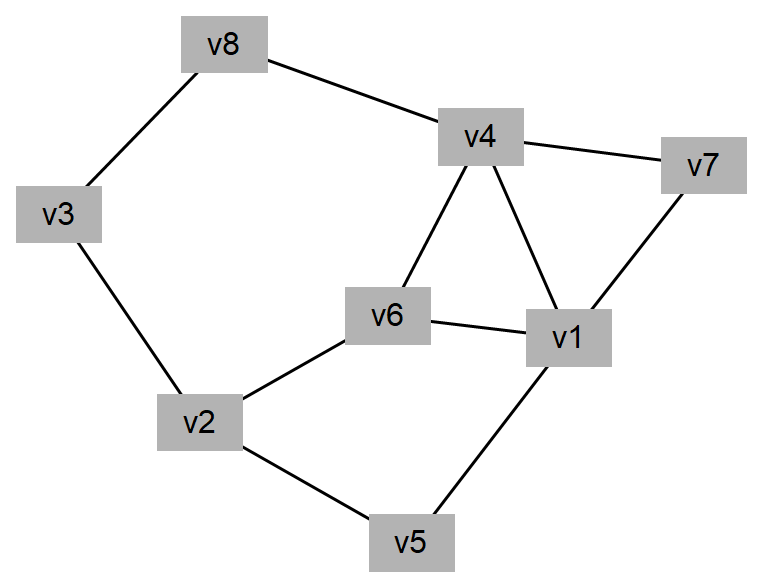
\includegraphics[width=0.33\linewidth]{images/primalgraph41.png}
	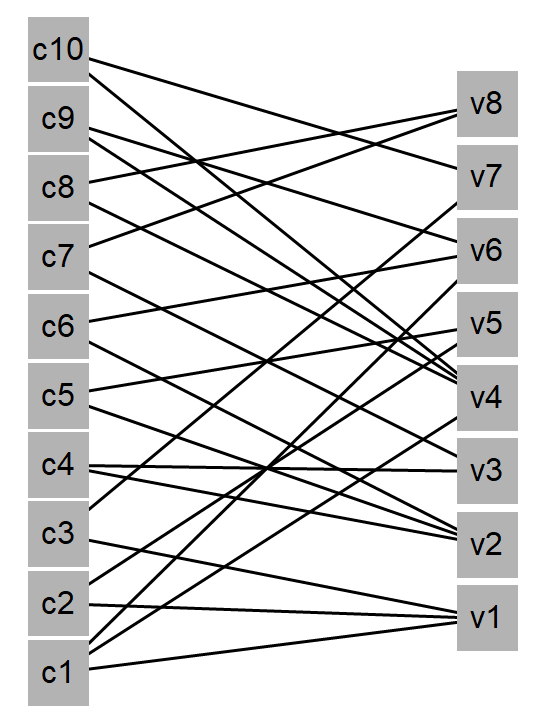
\includegraphics[width=0.32\linewidth]{images/incgraph41.png}
	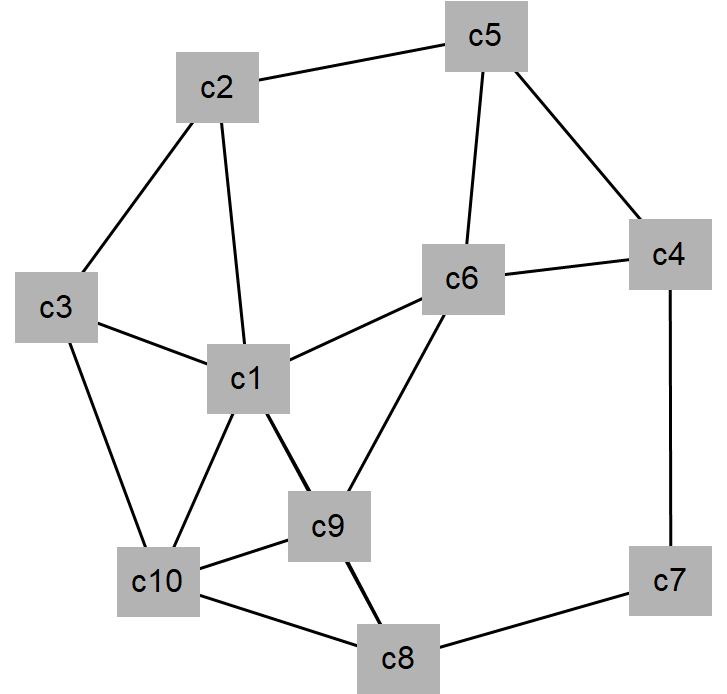
\includegraphics[width=0.33\linewidth]{images/dualgraph41.png}
	\caption{From left to right: primal, incidence and dual graph}
	\label{fig:primalgraph41}
\end{figure}

\subsubsection{From Propositional Logic to MSO Logic}

\textbf{First-order logic} adds relations and quantifiers to propositional logic.
For further information on logic see for example \cite[Chapter~5]{HandbookMathGraph}. \\
The quantifier symbols are
\begin{itemize}
	\item $\exists$ for the existential quantification and
	\item $\forall$ which expresses that a propositional function can be fulfilled by any member of a domain.
\end{itemize}

While first-order logic only quantifies variables that range over individuals (elements of the domain of discourse),
\textbf{Second-order logic}, in addition, also quantifies over relations.

\textbf{Monadic second-order logic (MSO)} is a restriction of second-order logic in which only quantification over unary relations (i.e. sets) is allowed. 
%A quantification over functions is therefore also not allowed due to the equivalence to relations.

%Interested in MSO logic over graphs.

%Two types of MSO formulas \textit{or logical graph representations}.
%The expressions have the form: ``There exists a \textbf{set of edges} that is..." can not be transferred into ``set of vertices".
%
%\begin{itemize}
%	\item MSO formulas
%	\item MSO$_{2}$ formulas with edge quantification $\equiv$ MSO formulas over incidence graphs
%\end{itemize}
%\begin{itemize}
%	\item G=(vertices, edges as binary relation)
%	\item INC(G) = (vertices and edges, Inc)
%	for G undirected: Inc(e,v) <-> v is a vertex of edge e
%\end{itemize}
%\begin{itemize}
%	\item FPT for clique width
%	\item FPT for tree-width
%\end{itemize}
%This can also be done for directed graphs!

% Applications

\subsubsection{MSO (Graph) Properties}
MSO logic can express graph properties and mappings from (labeled) graphs to (labeled) graphs \cite{CourcelleGROW}.
Typical MSO properties include:

\begin{itemize}
	\item \textbf{K-colorability}\\
	Example graph is 3-colorable:\\	
	$\exists X,Y~(X \cap Y = \emptyset \land \forall u,v~(edg(u,v) \implies [(u\in X \implies v\notin X)\land (u\in Y \implies v\notin Y)\land (u\notin X \cup Y \implies c \in X \cup Y)]))$
	
	\item \textbf{Connectivity}\\
	Example graph is \textbf{not} connected:\\	
	$\exists Z~(\exists x \in Z \land \exists y \notin Z \land (\forall u,v~[u\in Z \land edg(u,v) \implies v \in Z]))$
	
	\item \textbf{Vertex Cover} \cite[Ch. 4.2]{dpdbpadl2020}\\
	Given a graph $G=(V,E)$ a vertex cover is a set\\
	$C \subseteq V:edg(u,v)\implies \{u,v\}\cap C \neq \emptyset)$\\
	Then minimal vertex cover (MinVC) asks to find the minimum cardinality $|C|$ among all vertex covers of $G$. 
\end{itemize}

%\url{https://youtu.be/Wyn3djrYg7c?t=1385} Bruno Courcelle: Recognizable sets of graphs: algebraic and logical aspects 
%\url{https://library.cirm-math.fr/Record.htm?idlist=2&record=19276851124910940339}
%Recording during the thematic meeting: ``Frontiers of reconnaissability" the April 29, 2014 at the Centre International de Rencontres Mathématiques (Marseille, France)


%============== TD ====================================================
\subsection{Tree Decomposition}
%Used in RNA Folding: Novel prediction techniques are developed based on graph tree decomposition. \cite{BioInfoTD1970}
%See also chapter 2.2 of \cite{DiplomarbeitZisser}.
%Tree decompositions were originally introduced by Robertson and Seymour \cite{ROBERTSON198449} in 1984.
A \textit{tree decomposition} (TD) of a graph G is a pair $(T, \chi)$. $T$ is a tree and $\chi$ is a mapping which assigns each node $n~\in~V(T)$ 
a set $\chi(n) \subseteq V(G)$ called a \textit{bag}. Then $(T, \chi)$. $T$ is a TD if the following conditions hold:

\begin{itemize}
	\item[1.] for each vertex $v(n) \in V(G)$ there is a node $n \in V(T)$ such that $v \in \chi(n)$
	\item[2.] for each edge $(x,y) \in E(G)$ there is a node $n\in V(T)$ such that $x,y \in\chi(n)$
	\item[3.] if $x,y,z \in V(T)$ and $y$ lies on the path from x to z then $\chi(x) \cap \chi(z) \subseteq \chi(y)$. The set of bags that contain the variable v induce a connected sub-graph of T.
\end{itemize}
The width $width(T)$ of a tree decomposition $T$ is $max_{n\in V(T)}(|\chi(n)|)-1$.
The tree width of a graph is the \textit{minimal width} over all tree decompositions of the graph. 

%Wiki: In this definition, the size of the largest set is diminished by one in order to make the treewidth of a tree equal to one. 

MSO queries on tree decomposable structures are computable with linear delay \cite{MSOQueriesGuillaume}. There exist many ``easy" problems on tree decomposable graphs \cite{ARNBORG1991308}.

% Examples
We use tree decompositions throughout our visualizations in this thesis. One detailed explanation is also introduced in \cite{pcgp2019} at page 169.
The tree decomposition for our ``wheelgraph" example \ref{fig:wheelgraph} can be viewed in listing~\ref{lst:wheelgraphtd}. The conditions for tree decompositions outlined above are easy to verify for this small example, and we get a tree width $width(T)=3$ for this graph.

\begin{figure}
	\centering
	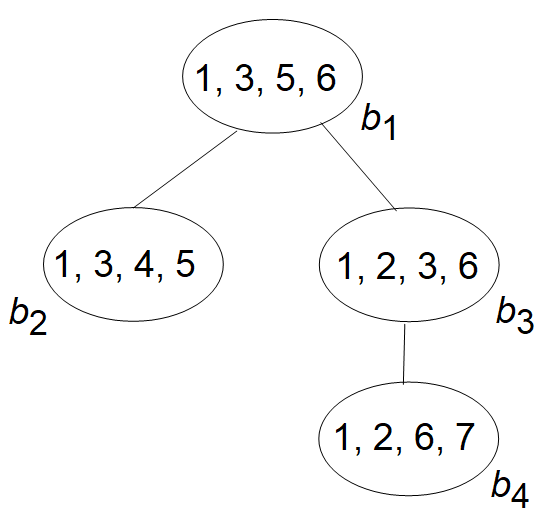
\includegraphics[]{images/TDWheelgraph7.png}
	\caption{Tree decomposition of a wheelgraph with 7 nodes and node 1 in the center.}
	\label{fig:tdweelgraph7}
\end{figure}

Some projects might use so called \textit{nice} tree decompositions in order to simplify the cases in the used algorithm \cite[Ch.~2.2]{DiplomarbeitZisser}.

As stated in \cite[Ch.~2.2]{DiplomarbeitZisser}, Arnborg et. al. \cite{arnborgtd} have shown that finding a tree decompositions of minimal width is only feasible for small graphs.  There are exact methods for obtaining minimal width tree decompositions,  e.g. \cite{gogatetw, bachoore06}. The solvers for which we implemented the visualization use heuristics  for  generating tree decompositions, therefore  the width of larger examples than shown in this thesis might not be minimal. 


%============== Reference on Algo and Param Complexity ====================================================
\subsection{Dynamic Programming on Tree Decompositions}
In this chapter we want to give a short overview over the basics of dynamic programming. For specific information on the visualized algorithms we refer to \cite{DiplomarbeitZisser, samermodelcounting, dpdbpadl2020}. \\

With dynamic programming, a problem is broken down into parts and the parts are then solved individually. The solving algorithm evaluates the formula along the path of the tree decomposition in a bottom up order starting in one of the leafs. The solution for each assignment in the bag is then stored in a table. The size of the table is exponential to the size of the bag. The tables of the child nodes can be deleted as soon as the table of the current node is generated. \cite[Ch. 3.1]{DiplomarbeitZisser}.\\

The dynamic programming approach for a given graph works as follows:
\begin{enumerate}
	\filbreak
	\item Create a tree decomposition ${T}$ of the graph.
	\item Apply dynamic programming for each bag in bottom up order of ${T}$
	\begin{itemize}
		\item[a)] visit the next node \textit{n} of ${T}$,
		\item[b)] apply the solving algorithm to the bag and
		\item[c)] store the results in a table.
	\end{itemize}
	\item Output the result based on the table of the root node of the tree decomposition.
\end{enumerate}

The basic algorithmic procedure is presented in Fig.~\ref{fig:dpalgo}. It does include a step one to build a graph in case the type of problem (like SAT) requires it.
\begin{figure}[h]
	\centering
	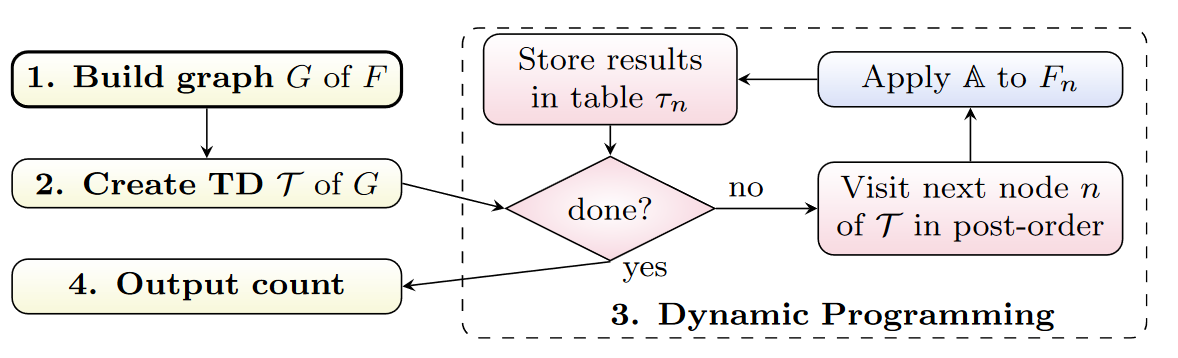
\includegraphics{images/DPAlgo31.png}
	\caption{ Basic procedure for dynamic programming on TD. \cite[Figure~3.1]{DiplomarbeitZisser} }
	\label{fig:dpalgo}
\end{figure}


\subsection{Parametrized Complexity}
In the following two sections we want to introduce the reader with some computational bounds for the underlying concept of solving MSO-problems with the current approaches.

\subsubsection{Fixed-Parameter Tractable (FTP-)Algorithm}

% https://en.wikipedia.org/wiki/Parameterized_complexity
\textbf{FPT for model checking}:
Some problems can be solved by algorithms that are exponential only in the size of a fixed parameter while polynomial in the size of the input. Such an algorithm is called a fixed-parameter tractable (FTP-)algorithm, and the problem can be solved efficiently for small values of the fixed parameter. \cite{ParamCompGrohe}
%\begin{thm}
%	An algorithm is FPT if it takes time $f(k)\cdot n^{c}$ for some constant $c$ and a fixed function f depending only on $k \in \mathbb{N}$. The size of the input is n. 
%	The value k is a parameter of the input, in our case usually tree-width. 
%	This algorithm is then usable for small values of k.
%\end{thm}

% Implications
There are efficient algorithms for enumerating and for counting the number of solutions of a MSO formula, if it is ensured that the input data is preprocessed in linear time, and that each solution is then produced in a delay linear in the size of each solution \cite{MSOQueriesGuillaume, ARNBORG1991308}.
MSO graph properties are ``fixed-parameter-tractable" with respect to tree-width. So are MSO counting and optimizing functions. \cite{CourcelleGROW}

DETAILS MinVC: 
%https://en.wikipedia.org/wiki/Vertex_cover#Fixed-parameter_tractability

%============== Courcelle ====================================================
\subsubsection{Courcelle's Theorem}
 Courcelle's theorem is a constructive meta-theorem and thus does provide algorithms for evaluating MSO formulas over graphs of bounded treewidth.
Courcelle's theorem \cite[p. 54]{Courcelle2012}:
\begin{thm}
	Every graph property definable in monadic second-order logic (MSO) is decidable in linear time on graphs of bounded tree-width. 

\end{thm}

\noindent
To be more specific: It holds that for all $k \in \mathbb{N}$ and MSO-formulas F is the decision problem for a given graph G, whether $G \models F$ is true, in time $2^{p(tw(G))} \cdot |G|$ with a polynomial p decidable.\smallskip 

\noindent
A generic workflow implementing Courcelle's theorem looks like we see in Figure~\ref{fig:UsageCourcelle}.
\begin{figure}[H]
	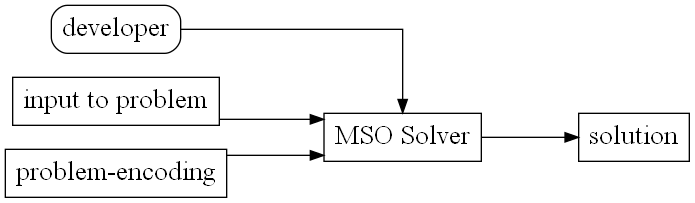
\includegraphics[height=0.2\textheight]{images/UsageCourcelle.gv.png}
	\caption{Implementation of the theorem}
	\label{fig:UsageCourcelle}
\end{figure}

Even if linear in the size of the input, naive implementations are still expensive and 
%($2^{p(tw G)}$, $2^{2^{(\#Q)}}$,  
the constant factor can be very significant. An efficient implementation will require several tricks to make this approach practical. Developing and debugging these ``tricks" is not always that easy, so a visualization can help at this point.\smallskip 

% See also figure~\ref{fig:logictheory}.
Auswirkung, Aktuelle Grenzen.

%==============================================================================
%============== Practical Requirements ========================================
%==============================================================================
\newpage
\section{Practical Requirements}\label{sec:practicalreq}
The exchange of intermediate results of solvers and parts of the visualization is done via two defined file formats. In the following two chapters we want to introduce the reader with the concepts of the DIMACS and DOT format. These formats are either produced or required as input at various stages of the application.
  
%============== DIMACS ====================================================
\subsection{DIMACS format}

Inputs for solvers and in some cases for preparing the visualization of dpdb are usually in a DIMACS format. There exist several standardized formats for different cases, for example CNF clauses, graph edges and graph decompositions.
Several file formats for these purposes were developed at ``DIMACS" (the Center for Discrete Mathematics and Theoretical Computer Science) \cite{dimacsimplcha} beginning in 1993 at Rutgers University.
They are partly supported in several math-related software.

The underlying concept is one line-based ASCII file and for all different formats specifies comments as lines starting with the character ``c", a problem line starting with ``p" (rarely with ``s") and following the problem line usually multiple lines specifying the data in a format depending on the problem type.
The formats used for this work are:

\textbf{DIMACS CNF}: This format is used to define a Boolean expression, written in conjunctive normal form. The problem line specifies the type, \textbf{number of variables} and \textbf{number of clauses}. The following lines specify the clauses a positive literal is denoted by the corresponding number, and a negative literal is denoted by the corresponding negative number. Each clause is followed by the character zero, so 0 should not occur as a variable. Instead variables are expected to start at one.\\

\textbf{DIMACS tw}: This format is used to describe a single undirected graph. The problem line specifies the type, \textbf{number of nodes} and \textbf{number of edges}. The following lines specify the edges with two nodes separated by a space.\\

\textbf{DIMACS td}: This format is used to describe a tree decomposition. The problem line specifies the type, \textbf{number of bags}, \textbf{maximum size of the bags} and \textbf{number of nodes}. The following lines describe the bags starting for each with ``b", the \textbf{bag number} and \textbf{nodes in this bag}. Following these bags are lines not prefixed with a ``b". Now each line describes one \textbf{edge between the bags} as two bag numbers separated by a space.\\

%Supported also in Maple \url{https://www.maplesoft.com/support/help/maple/view.aspx?path=Formats/CNF}

Some examples of this format can be seen in the appendix on page \pageref{app:input}.

%============== DOT ====================================================
\subsection{DOT format}
The graph description language DOT can be used to describe directed or undirected graphs and specify layout details and various attributes for graphs, edges and nodes. It is similar to the Graph Modeling Language that is used in Chapter \ref{chagraphoutput} as a text based file format for describing graphs. The \href{https://graphviz.org/}{Graphviz} project includes gml2gv and gv2gml as two tools that can convert between GML and DOT files. Keeping this in mind, in this chapter we restrict ourselves to a short introduction of the DOT properties that were used the most.

%=========================== DOT Language ====================================

%Dot Language: http://www.graphviz.org/doc/info/lang.html

The complete abstract grammar for DOT can be viewed at the website of the DOT language \url{https://graphviz.gitlab.io/_pages/doc/info/lang.html}.\\


The nodes in the DOT-language are \emph{labeled}, so creating a node takes one string identifier and might additionally be provided with a text label. Valid examples for IDs include all combinations of letters and digits.

The optional text labels an have various formats. One example with the setting ``shape=box''

%It supports directed (\textit{digraph} with edges indicated by '->') an undirected (\textit{graph} with edges indicated by '-{}-') graphs.
The visualizations presented in the thesis are constructed as undirected graphs, but would be easily extendable to directed representations, since the order of the edge endpoints remains intact in almost all operations.

Another concept utilized were the sub-graphs and clusters available in DOT.
To get a well structured (bipartite) incidence graph, each partition is placed in an individual cluster, making adjustments to various distances simple.\\


%Attributes (new site): http://www.graphviz.org/doc/info/attrs.html
DOT has different components (see \url{http://www.graphviz.org/doc/info/attrs.html}) which can be modified with attributes: edges, nodes, the root graph, subgraphs and cluster subgraphs, respectively.\\


We want to introduce the reader with the attributes that are modifiable in several places of the visualization:

\begin{itemize}
	\item \textbf{rankdir -} ``TB", ``LR", ``BT", ``RL", corresponding to directed graphs drawn from top to bottom, from left to right, from bottom to top, and from right to left, respectively.
	
	\item \textbf{fillcolor -} The color used as a node-background in different situations, for different values see \url{https://graphviz.org/doc/info/attrs.html#k:color}. \url{https://graphviz.org/doc/info/colors.html} 
	By default this is a linear fill; If the value is a colorList, a gradient fill is used. 
	
	\item \textbf{fontcolor -} Color for text in nodes or graphs. 
	
	\item \textbf{style -} Drawing style of the nodes.
	At present, the recognized style names are ``dashed", ``dotted", ``solid", ``invis" and ``bold" \textbf{for nodes and edges},  and ``filled", ``striped", ``wedged", ``diagonals" and ``rounded" \textbf{for nodes} only.
	
	\item 
	\textbf{margin -} Used for horizontal and vertical margins around graphs.
	
	\item \textbf{fontsize -} Font size, in points. 
	
	\item \textbf{penwidth -} Specifies the width of the pen in points. This is used to draw lines and curves, including the boundaries of edges and clusters. 
	
	\item \textbf{nodesep -} In dot, this specifies the minimum space between two adjacent nodes in the same rank in inches. 
	
	\item \textbf{shape -} Controls how nodes are drawn. For a full list of shapes see \url{https://graphviz.org/doc/info/shapes.html}. There are three main ways of specifying shapes, and all are applied in our visualization: 
	\begin{enumerate}[label=(\arabic*)]
		\item \textbf{polygon-based}; for example as a box, ellipse or diamond.\vspace{10pt}\\		
		\textbf{Example}: shape~=~diamond label~=~v\_1
		
		\item \textbf{record-based} nodes that are basically boxes stacked vertically and horizontally and each filled with text.\vspace{10pt}\\
		\textbf{Example}: shape~=~record label~=~$\{\text{sol bag 2}|\{\{v1|1|1|1|1|0\}|\{v3|1|0|0|1|1\}$ \\
		\hspace*{0pt}\hfill $|\{v5|0|1|0|1|1\}|
		\{\text{size}|3|3|2|3|3\}\}|\text{min-size: 2}\}$
		
		\item \textbf{HTML-like} labels are specified in a own grammar and can contain tables, text-styles like italic, sub- and superscript, vertical and horizontal rules.\vspace{10pt}\\		
		\textbf{Example}: shape~=~box label~=\vspace{5pt}\\
		$<<$TABLE BORDER="0" CELLBORDER="0" CELLSPACING="0"$>$\\
		$<$TR$><$TD BGCOLOR="white"$>$bag 1$<$/TD$><$/TR$>$\\
		$<$TR$><$TD PORT="anchor"$>$$<$/TD$><$/TR$><$TR$><$TD$>$[1, 3, 5, 6]$<$/TD$>$\\ $<$/TR$><$TR$><$TD$>$dtime=0.0009s$<$/TD$><$/TR$><$/TABLE$>>$
	\end{enumerate}
\end{itemize}


%==============================================================================
%============== PROJECT =======================================================
%==============================================================================
\newpage
\section{Implementation}\label{sec:project}

In this section we want to give a thorough insight into the functionalities of TDVisu.\\

\noindent As a rough overview our software TDVisu works as follows:

\begin{enumerate}
	\item We generate data using a special solver extension or extra programs and extract arguments for the visualization into one file following our JSON schema.
	\item We read the data and parameters into the visualization.
	\item The program creates a graph-layout for the bags of the tree decomposition and calculates which parts are to be shown at each step of the provided solving process.
	\item It creates a graph-layout for each additional graph to visualize alongside the steps in the tree decomposition.
	\item Each graph for individual time steps is saved as a SVG file.
	\item If desired, the individual parts of a time step can be merged into a single SVG file.
\end{enumerate}

The programming language chosen is Python because of it's rich dependency environment, fast prototyping, simple tooling for debugging with pdb, optional static analysis with mypy, easy to follow code-style using pylint and autopep8, and modern packaging with pip and pypi.

Python 3.8 was the newest python version at the beginning of the project, released on October 14th 2019. The innovation most frequently applied in this project was the f-string support for shorter and easier to read string-building. %\href{https://docs.python.org/3/whatsnew/3.8.html}{summary of release highlights}.

The development process was for most parts of the final software driven by evolutionary prototyping with the help of small and well understood examples such as \ref{fig:g41Digraph}. It helped to understand the possibilities of visualization in this domain and gather user input and requirements early \cite{rapidPrototypingOvermyer}. Some artifacts of the early prototypes with different graph-description languages can be still seen in the class \textit{Graphoutput} in \ref{chagraphoutput}.

The first versions were developed in the repository \url{https://github.com/VaeterchenFrost/gpusat-VISU} and the first releases and later development of the source code was outsourced to the \url{https://github.com/VaeterchenFrost/tdvisu} repository.

% License

% Files / Classes / Methods
%============== CMD Config ====================================================
\subsection{Commandline and Configuration}

The \textit{tdvisu.visualization} expects the command line parameters in a format described by Table~\ref{tab:optionstdvisu}.

\def\arraystretch{1.2}%  1 is the default
\begin{longtable}{|ll|}
	\caption{Usage visualization.py 
		\label{tab:optionstdvisu}}\\
	\hline 
	\multicolumn{2}{|c|}{[-h] [--version] [--loglevel LOGLEVEL] [infile] outfolder}
	\\[2ex]
	\endfirsthead

	infile=stdin &  Input file for the visualization must conform with the JsonAPI.md\\
	outfolder &  Foldername to output the visualization results to\\
	-{}-loglevel  &   set the minimal loglevel for the root logger\\
	-{}-version & show program's version number and exit\\
	-h, -{}-help & show the help message and exit\\
	\hline
\end{longtable}

We see that this input is very simple, and that the heavy lifting is done with the input file given in \textit{infile}.

One extra possibility for configuration comes with the method \textbf{logging\_cfg} from {tdvisu.utilities}. There are two example configurations provided with our project, one in the .yml, one in the .ini format. The implementation is very flexible in detecting which parser has to be applied - either via a dictionary-like or a configuration-like function. Both possibilities are documented in python's \href{https://docs.python.org/3/library/logging.config.html#logging-config-api}{logging configuration}.

Our default configuration in tdvisu/logging.yml and tdvisu/logging.ini provides one handler, two formatters and six loggers.

The \textbf{handler} is a stream handler to sys.stdout with level \textit{WARNING} and the the 'full'-formatter to format messages.

The \textbf{full-formatter} includes the full date and time up to milliseconds. After that we can expect the logging-level, filename and line where it was generated, and the message itself.

The \textbf{loggers} we use in our project are located in 
\begin{itemize}
	\item root, level: WARNING
	\item visualization.py, NOTSET
	\item svgjoin.py, NOTSET
    \item reader.py, NOTSET
	\item construct\_dpdb\_visu.py, NOTSET
	\item utilities.py, NOTSET
\end{itemize}
and can be individually customized using one configuration file.
With the command line parameter \textit{-{}-loglevel} we can modify the level of \textit{root} and it's associated handlers.

%============== Init ====================================================
\subsection{Initialization and Tree Decomposition}

To get a small overview of the type and structure of the data processed in the software, let's take a quick look at the initialization with the API. We instantiate a Visualization object as shown in Listing~\ref{lst:visuinitsmall} , which parses the \textit{VisualizationData} with the help from our \textit{inspect\_json} method. 

The main purpose of the initialization is parsing the input file containing visualization information.
%This is encapsulated in \textit{read\_json}.

Next we want to extract information into several objects: 
\begin{itemize}
	\item the instance variables 
	\begin{itemize}
		\item \textit{timeline}, describing the time steps on the tree decomposition
		\item \textit{tree\_dec}, describing the TD itself
		\item \textit{bagpre}, \textit{joinpre}, \textit{solpre} and \textit{soljoinpre} as names for different nodes in the produced visualization
	\end{itemize}
	\item The \textit{VisualizationData} object containing the data for 
	\begin{itemize}
		\item IncidenceGraphData in Listing~\ref{lst:incidencedata} p. \pageref{lst:incidencedata}
		\item GeneralGraphData in \ref{lst:gengraphdata} p. \pageref{lst:gengraphdata}
		\item SvgJoinData in \ref{lst:svgjoindataclass} p. \pageref{lst:svgjoindataclass}
		\item adjustable parameters, which influence additional aspects of the visualization
	\end{itemize}
\end{itemize}


\begin{lstlisting}[language={Python}, caption={Overview of data initialization}, label={lst:visuinitsmall}]
def __init__(self, infile, outfolder) -> None:
	self.data: VisualizationData = self.inspect_json(infile)
	self.outfolder = outfolder
	self.tree_dec_digraph = None
	
def inspect_json(self, infile) -> VisualizationData:
	visudata = read_json(infile)
	
	[...]
	_incid = visudata['incidenceGraph']
	_general_graph = visudata['generalGraph']
	_svg_join = visudata.get('svg_join', None)
	
	[...]
		
	return VisualizationData(incidence_graph=incid_data,
													 general_graph=general_graph_data,
													 svg_join=svg_join_data,
													 **visudata)
\end{lstlisting}


Our next step is to begin visualizing the time-steps on the tree decomposition in \textit{Visualization.tree\_dec\_timeline}.\\

First, a quick setup is performed for the tree decomposition as a directed graph that 
\begin{itemize}
	\item is \textit{strict}, meaning a simple graph where equal edges are merged into one
	\item has an orientation where it grows with each ``rank" of the nodes
	\item has a shape and a fill-color for it's nodes
	\item has a margin around it's bounding box.
\end{itemize}

Second, it creates the basic bag structure by adding nodes and edges for all bags of the provided tree decomposition.

Next comes the iteration over the time steps, adding the provided solutions and the edges connecting them to the existing bags. We do this in two passes.  A first in which we move all the nodes into their final position. And one in which we create the actual time step images backwards by masking later calculated solutions. The goal is to have all parts of the graph in optimal position when they first appear and not to move when additional features are added. Details of this pass can be seen in listing \ref{lst:backward-iterate} on page \pageref{lst:backward-iterate}.\\

A special case occurs when two bags are joined together.

In this case, we remove all old edges between the children and the parent node, add the link result to the graph, and add edges from the children to the link result and from the link result to the parent node. Details of this function can be seen in Listing~\ref{lst:forward-iterate} on page \pageref{lst:forward-iterate}.

An automatically inserted join node is shown in Figure~\ref{fig:g41Digraph} p. \pageref{fig:g41Digraph}.
The provided data for this example to layout the bags can be seen in Listing\ref{lst:edgearray41} on page \pageref{lst:edgearray41}. Here we see that bags 2 and 3 have an edge to bag 1 and therefore a join-operation will occur between the results of bags 2 and 3:

\begin{lstlisting}[caption={Structure provided for bags of example \ref{fig:g41Digraph} },label={lst:edgearray41},numbers=none,backgroundcolor=\color{white}]
"edgearray" : 
[
	[ 1, 0 ],
	[ 2, 1 ],
	[ 3, 1 ],
	[ 4, 3 ]
]
\end{lstlisting}

For rendering the tree decomposition we have added a convenience option to \textit{view} the result files automatically (disabled by default).

%============== Timesteps ====================================================
\subsection{Create time steps for the underlying graph}
To gain a more comprehensive insight into the solution process, we have illustrated in the same way the diagrams that best describe the problem instance the solver has been working on.

Because the data in the API does not directly include details about highlights in those graphs, we will construct this information on the fly by referencing with the tree decomposition.

With additional data from the \textit{IncidenceGraphData} class we are further able to reconstruct the
\begin{itemize}
	\item incidence graph,
	\item primal graph,
	\item dual graph
\end{itemize}
for Boolean formulas.

For general problems and with the data from the \textit{GeneralGraphData} class we can construct a simple graph that logically should include the nodes which are in the bags of the TD.\\


% ----- Example for isolated nodes -------
Because graph representations of Boolean formulas are not necessarily connected, we make sure to include potentially isolated nodes into our graphs as well and not only draw some components of it.
For example the formula \\
$(\neg a\lor \neg b\lor \neg c\lor \neg d)\land (b\lor c\lor d)\land g$\\

with its set of clauses \\
$\{c_{1}=\{-a,-b,-c,-d\},c_{2}=\{b,c,d\},c_{3}=\{g\}\}$ \\
will create the dual graph in Fig. \ref{fig:disconnected123}. This happens with no pre-processing and if the variable g is only included in the unit $c_{3}$.

\begin{figure}[H]
	\centering
	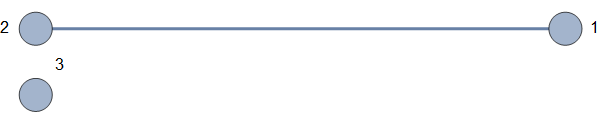
\includegraphics{images/disconnected123.png}
	\caption{Disconnected (dual) graph}
	\label{fig:disconnected123}
\end{figure}

%============== Incid ====================================================
\subsection{Incidence Graph}\label{sec:incid}

The idea is to visualize the incidence graph as a bipartite graph that can represent the formula for which it was created.

\begin{figure}[H]
	\centering
	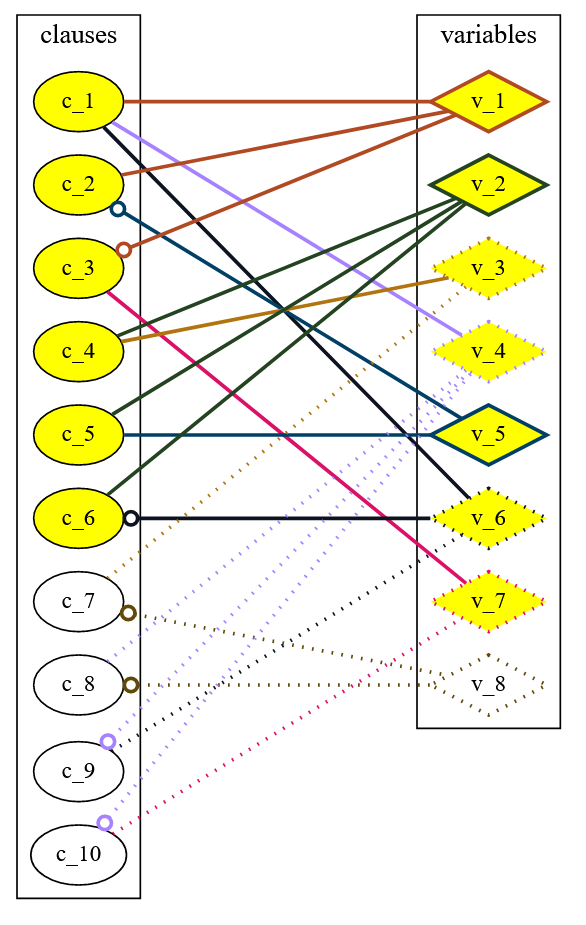
\includegraphics[width=0.4\linewidth]{images/IncidenceStep6.png}
	\caption{Example for the incidence graph constructed from Ex. \ref{ex:example41}.}
	\label{fig:incidencestep6}
\end{figure}

 We can see the incidence graph visualization for our example Boolean formula in Figure~\ref{fig:incidencestep6}. On the left side we see the clauses ordered by their label, each in an ellipse-shaped node. The other partition does contain the sorted variables in diamond-shaped nodes. As an addition to its visualization we did include the negations as the little circles on the left end of each edge where a negated variable is included in the respective clause. The right-hand partition does get the different \textit{colors} applied to its nodes and their adjacent edges.
 
 We emphasize the clauses their nodes used in each timestep with a changing background and the not used dotted edges. This allows the correlation of the  parts of the formula with the bags.  

The representation of the bipartite graphs can be adjusted in many parameters; including colors, fontsize, fillcolor and more, Listing \ref{lst:incidencedata} on page \pageref{lst:incidencedata}.

%We create the graph, add the necessary arguments and two sub-graphs. 
%The first subgraph is called \textit{cluster\_clause} with it's label \textit{clauses}.
%We add the clauses with their clause-ids starting at one sorted in ascending order from top to bottom.

%The second sub-graph we call \textit{cluster\_ivar} labeled \textit{variables} gets all variables added to it, 
%starting from variable-id one. 
%This sub-graph does get the different provided \textit{colors} applied to its nodes and their adjacent edges.

%The last step in this method is the highlighting of ``active" parts in each time step beeing processed during it's dynamic programming. To accomplish this with as small overhead as possible, we apply and remove additional lines to the body of its graph source code. 
%For highlighting there are two main cases:
%\begin{itemize}
%	\item There is no active clause in this step: we only reset highlighting
%	\item Else: we also create new highlighting for clauses, variables and edges
%\end{itemize}
%In each case we create one image after the step to provide the inside generated.

%============== General Graph ====================================================
\subsection{General Graph}
This type of graph can represent the underlying graph for different problems, as well as primal and dual graph for Boolean formulas.
Because of its wider scope, the layout for the general graph was not as simple to create as for the incidence graph.
We did prepare two different layouts that should cover most cases and are toggled by the parameter \textit{do\_sort\_nodes}.
For smaller and dense graphs of up to 20 vertices it might be helpful to sort the nodes on a circle, while for larger or sparse graphs an organic layout may be more appropriate.

To layout these two options we chose the engine 
\begin{itemize}
	\item \textit{do\_sort\_nodes} true: circo (see \cite{ST99})
	\item \textit{do\_sort\_nodes} false: sfdp (see \cite{Hu05}) with the spring constant 'K' set to 2.
\end{itemize}

Additional parameters used in both layouts are used to not overlap nodes, as well as drawing the edges first. This should provide a minimally cluttered layout compared to the defaults, but could make edges ambiguous in some cases. \\
%
%Of course these layouts could process even more configuration, a complete overview can be found in the \href{https://graphviz.org/doc/info/attrs.html}{graphviz-doc}. 

%Only if the option to sort the nodes was chosen with \textit{do\_sort\_nodes} the method
%\begin{enumerate}
%	\item saves the current graph source 
%	\item sets the layout engine to \textit{circo}
%	\item adds edges between successive node-ids to form a closed circle
%	\item runs the layout and reads back the output in plain dot-format
%	\item reads the calculated positions for each node in the graph
%	\item resets the source to step one, removing all temporary additions
%	\item writes the calculated positions into each node
%	\item sets the layout engine to an engine that uses those calculated positions later.
%\end{enumerate}

%We add the edges and eventually the isolated nodes to the graph.
The highlighting for each time step is basically the same as in the incidence graph previously.\\

We allow an additional option, which depends on the concrete algorithm to be visualized, namely the flag \textit{do\_adj\_nodes}.
In case the algorithm uses adjacent nodes they can be visualized with this flag using a third color for emphasis.\\


% --- EXAMPLE
A more detailed presentation of the results with these visualizations is presented in Section \ref{sec:minvc}.
Figure \ref{fig:minvc16graph9} shows a graph visualization for a graph with 16 nodes and the subgraph $\{11,12,14\}$ emphasized.\\
Figure \ref{fig:minvc16graph9sorted} shows the same graph and emphasis visualized with the nodes sorted and placed on a circular layout. In this layout we find it easier to identify individual nodes by their position and to cross-reference them with further representations.

\begin{figure}[H]
	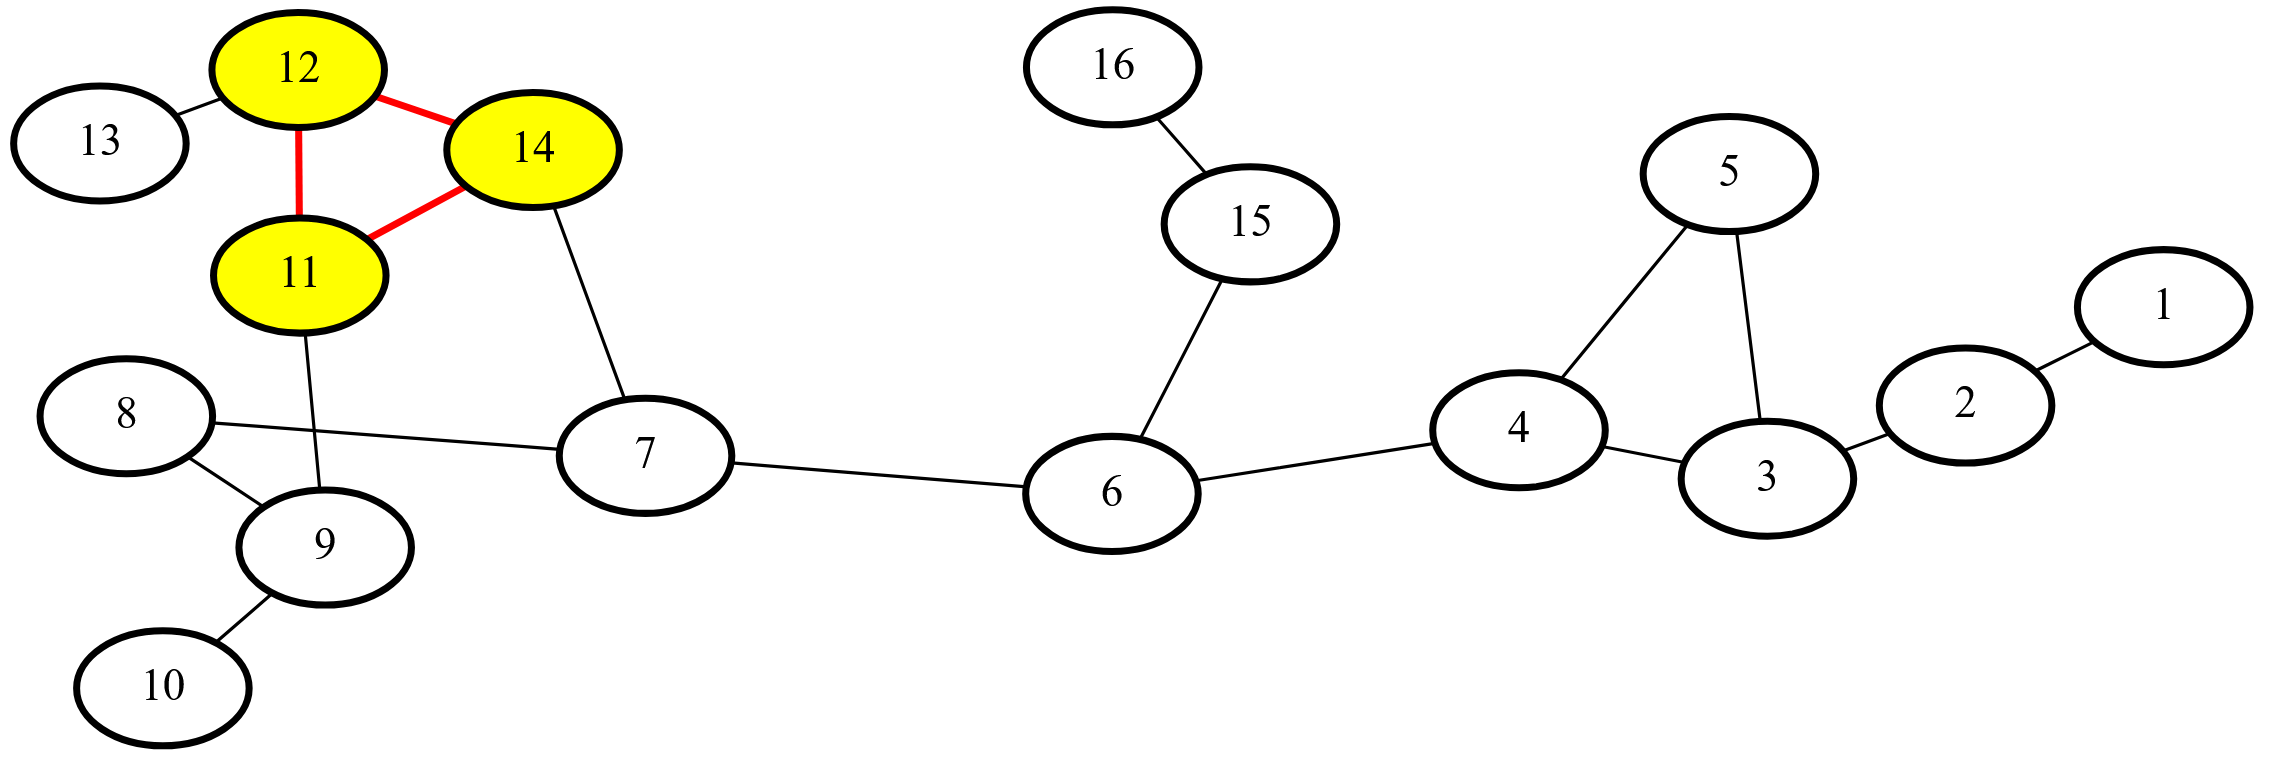
\includegraphics[width=\linewidth]{images/minvc16graph9.png}
	\caption{A graph with 16 nodes and highlights for the subgraph $\{11,12,14\}$ in yellow and red edges.}
	\label{fig:minvc16graph9}
\end{figure}

\begin{figure}[H]
	\centering
	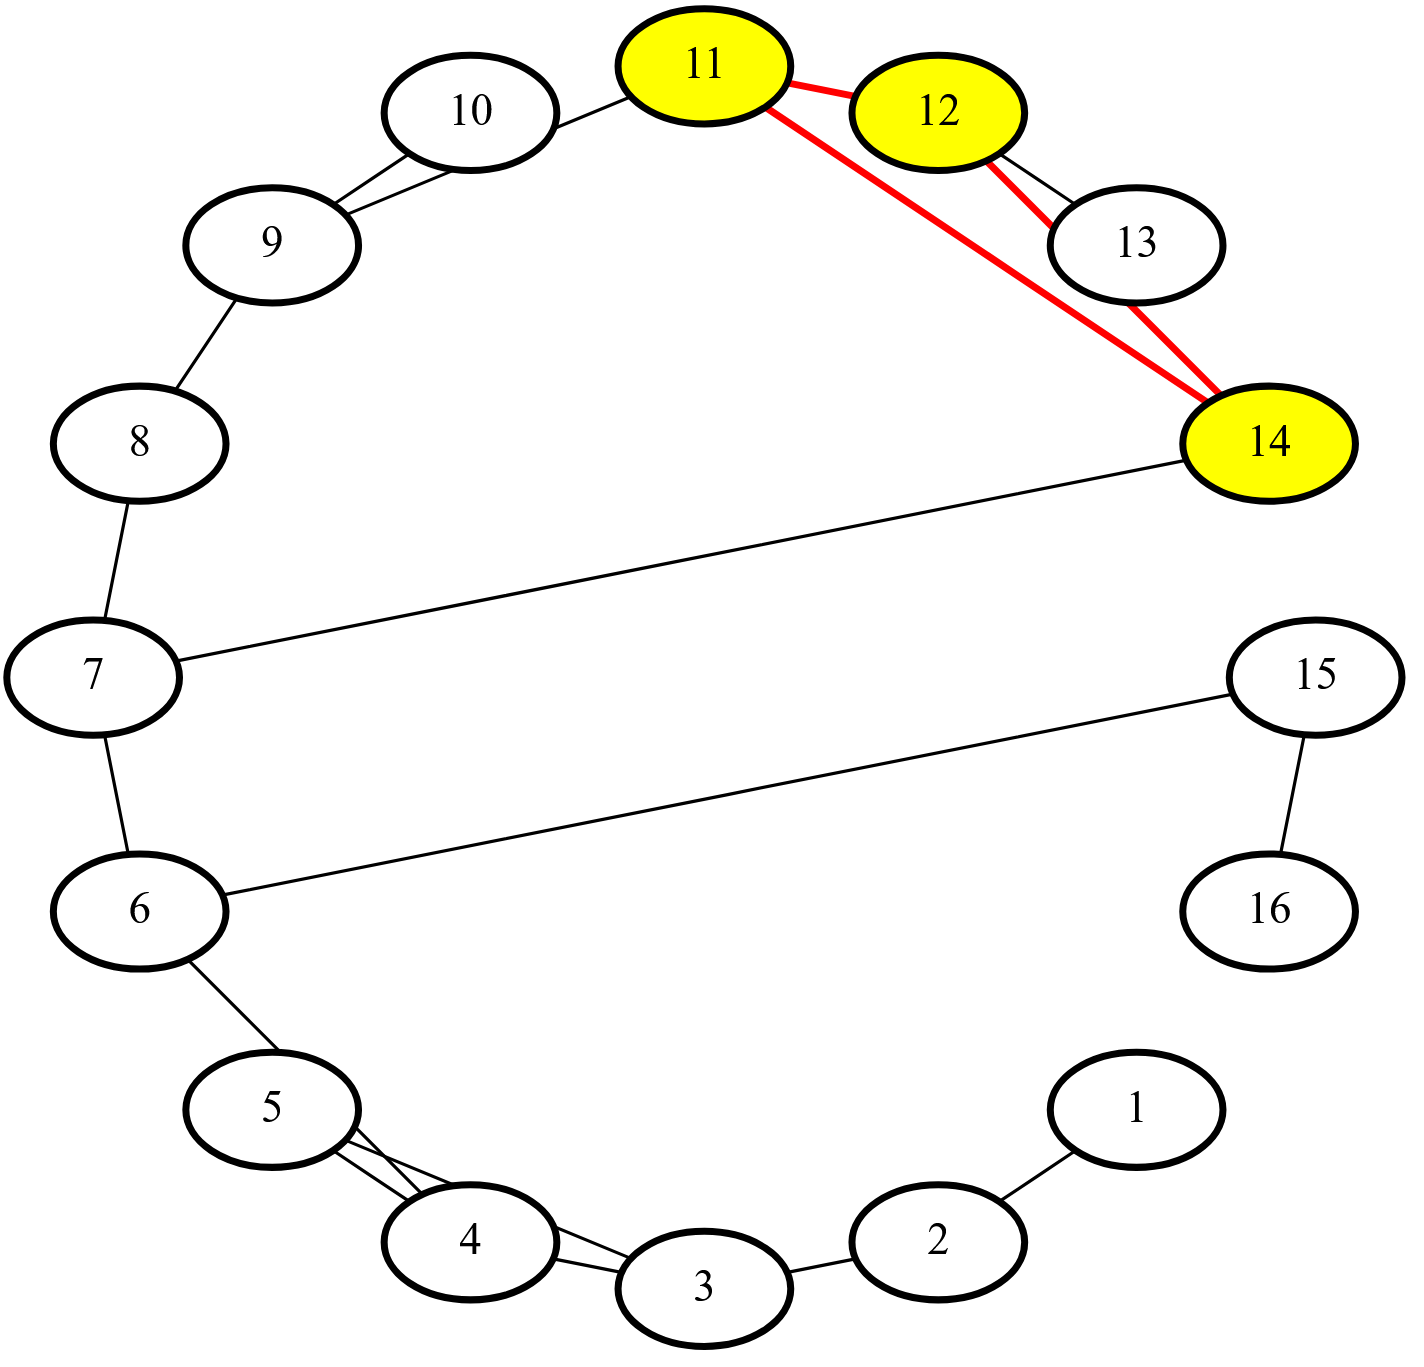
\includegraphics[width=0.6\linewidth]{images/minvc16graph9sorted.png}
	\caption{A graph with 16 nodes and highlights for the subgraph $\{11,12,14\}$ in yellow and red edges. The nodes are arranged in a circular layout and sorted by their labels.}
	\label{fig:minvc16graph9sorted}
\end{figure}

%============== Joining SVG ====================================================
\subsection{Joining SVG}\label{sec:svgjoin}
Once all user defined images for one timeline are created, it would be nice to have all graphs combined in one file for each step.
To support this functionality and some basic scaling and adjusting, we prepared a section in the API for joining the resulting SVG graphs. 
This functionality is placed in the file \textit{svgjoin.py} and will be called with the specifications given in the optional dictionary \textbf{svgjoin} within the JsonAPI.

The parameters can be viewed in \textit{SvgJoinData} in Listing \ref{lst:svgjoindata} on page \pageref{lst:svgjoindata}.\\

% Show example with description of parameters 
%The internally used method \textit{svgjoin.append\_svg} joins two images horizontally in each step.
With default settings it will align the top of both images and apply no scaling to either of them.
The possible parameters (in [unit])
\begin{itemize}
	\item centerpad: float = 0, [image coordinates], just ``padding" in the JSON API
	\item v\_bottom: float = None, [size of the \textit{first} image]
	\item v\_top: float = None, [size of the \textit{first} image]
	\item scale2: float = 1, [size of the \textit{second} image]
\end{itemize}
allow flexible \textbf{vertical}, \textbf{horizontal} and \textbf{scaling} transformations.
Note that the images are placed in a Cartesian coordinate system and their origin is the upper left corner of their bounding box. All images fill a rectangle in this coordinate system with height and width respectively.

Since the order of the parameters \textit{v\_bottom} and \textit{v\_top} could be confused due to the inverted y-axis, we make sure that \textit{v\_top} is correctly set to the smaller and \textit{v\_bottom} to the larger value whenever possible.

A special case is achieved by setting both parameters to the same number. Then they are interpreted as the position of the vertical centerline for the second image in units of the first. So setting both parameters to $\dfrac{1}{2}$ would result in both images being vertically centered.\\

Possibilities for joining images with these four parameters include joining with:
\begin{itemize}[label=-, left=40pt]
	\item default \textit{centerpad}, Fig. \ref{fig:svgjoinpad0}.
	\item \textit{centerpad} set to 200, Fig. \ref{fig:svgjoinpad200}.
	\item scaling both images to the same size, Fig. \ref{fig:svgjoinscale1}.
	\item aligning both images for vertical centering, Fig. \ref{fig:svgjoinpad0centered}.
	\item uniformly scaling the second image, Fig. \ref{fig:svgjoinscaled}.
	\item scaling and aligning at the bottom edge of the image, Fig. \ref{fig:svgjoinscaledbottom}.
\end{itemize}

\begin{figure}[H]
	\centering
	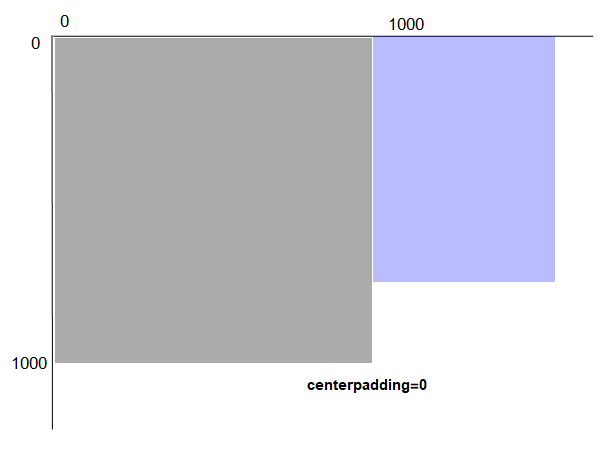
\includegraphics[width=0.6\linewidth]{images/svgjoinpad0.png}
	\caption{Example for joining with no \textit{centerpad}.}
	\label{fig:svgjoinpad0}
\end{figure}

\begin{figure}[H]
	\centering
	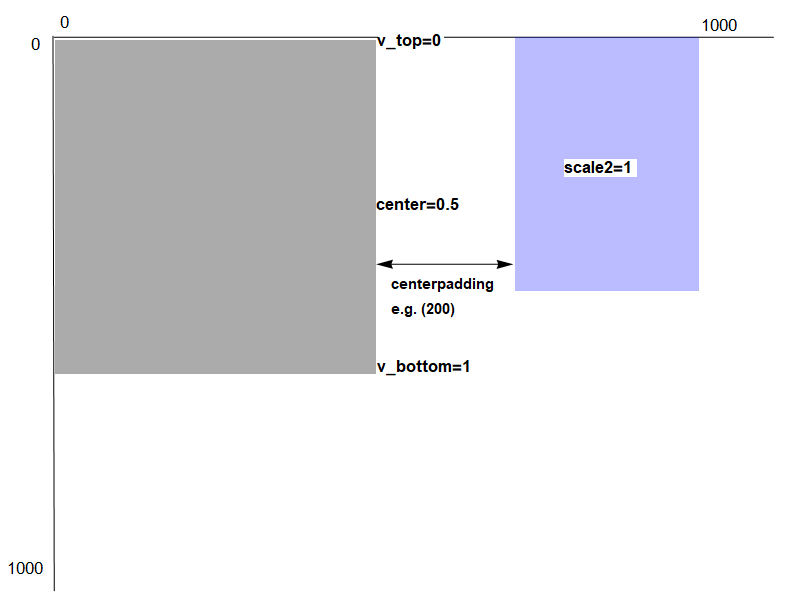
\includegraphics[width=0.8\linewidth]{images/svgjoinpad200.png}
	\caption{Joining the blue (right side) image to the left gray image with only one parameter \textit{centerpad} set to 200. We see the default vertical position v\_top=0, and the implied coordinate system with an origin in the top left corner.}
	\label{fig:svgjoinpad200}
\end{figure}

\begin{figure}[H]
	\centering
	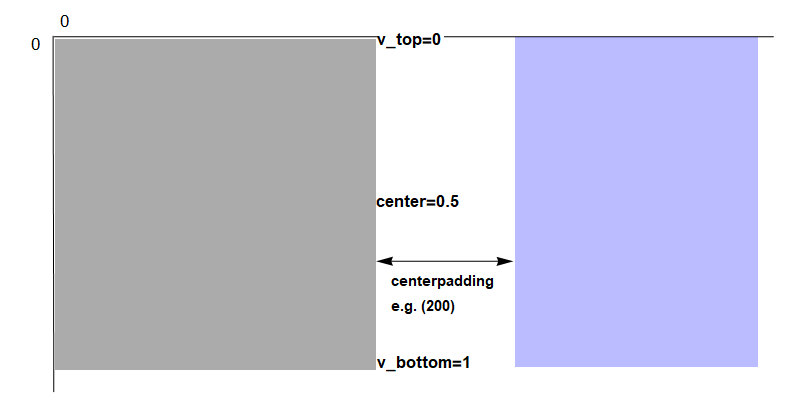
\includegraphics[width=0.8\linewidth]{images/svgjoinscale1.png}
	\caption{The second image is scaled to the same size as the first image. This can be conveniently achieved by setting \textit{v\_top} to 0 and \textit{v\_bottom} to 1. Parameter \textit{centerpad} is 200 as hinted.}
	\label{fig:svgjoinscale1}
\end{figure}

\begin{figure}[H]
	\centering
	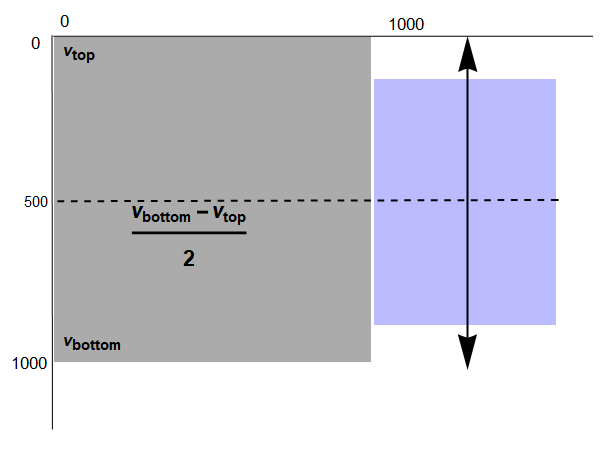
\includegraphics[width=0.8\linewidth]{images/svgjoinpad0centered.png}
	\caption{Align both images for vertical centering. \\
		This can be achieved by setting $v\_bottom=v\_top=0.5$.}
	\label{fig:svgjoinpad0centered}
\end{figure}

\begin{figure}[H]
	\centering
	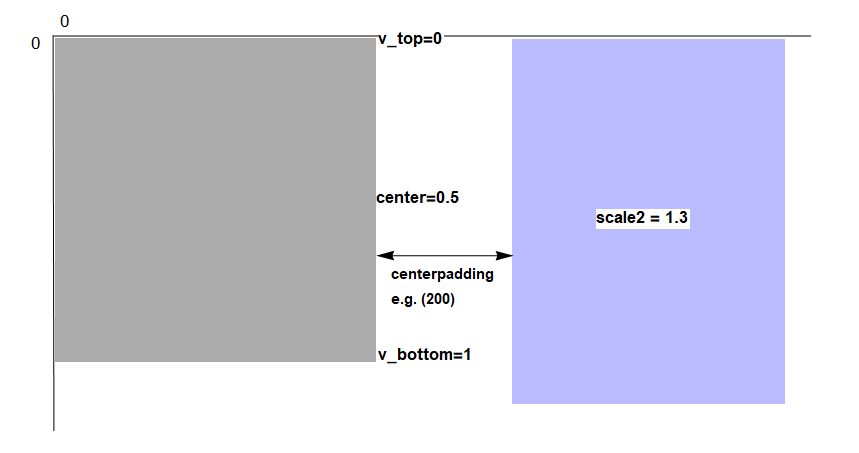
\includegraphics[width=0.8\linewidth]{images/svgjoinscaled.png}
	\caption{Setting \textit{scale2} to $1.3$ to scale the blue (right) image uniformly. Parameter \textit{centerpad} is 200 as hinted.}
	\label{fig:svgjoinscaled}
\end{figure}

\begin{figure}[H]
	\centering
	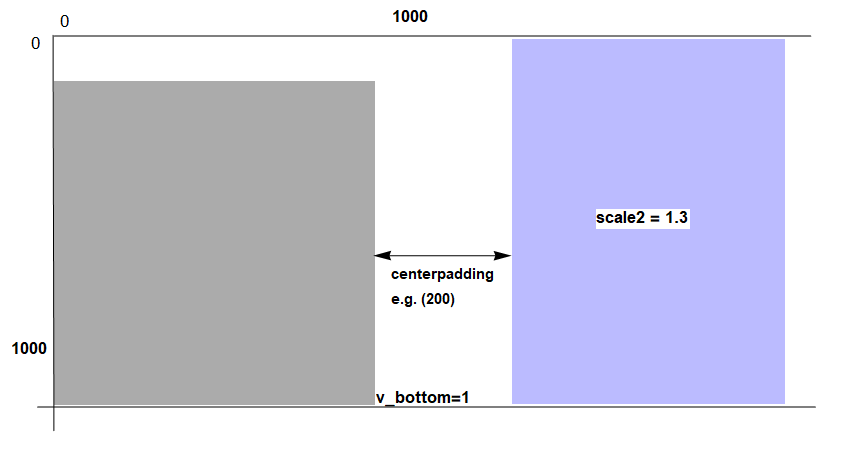
\includegraphics[width=0.8\linewidth]{images/svgjoinscaledbottom.png}
	\caption{As in figure \ref{fig:svgjoinscaled} we use \textit{scale2} to scale the blue rectangle. To align both images at the bottom edge, we use the value $v\_bottom=1$.}
	\label{fig:svgjoinscaledbottom}
\end{figure}

If we want to merge more than two images, it is possible to specify the parameters in a list.
The list can be of different length for each parameter - if it is exhausted, the last parameter in the list will be repeatedly used until all images are joined together.

%==============================================================================
%============== GPUSAT ========================================================
%==============================================================================
\newpage
\section{Integration in GPUSAT}\label{sec:gpusat}
%To study and improve the handling of the C++ program was chronologically the first task we experimented with.
%Getting the program up and running proved to be more difficult than we envisioned due to a probable bug in the driver when running OpenCL Drivers from CUDA on the Windows OS.

The integration of visualization into the C++ based \url{https://github.com/daajoe/GPUSAT} did happen in two parts. \\

The first part is mostly included in the class \textit{Graphoutput}, and includes several experimental steps into visualization. This class has 186 lines of code (LOC) in its source file, and 44 lines of code in its header file.

The second part was done in the class \textit{Visualization}, and fulfills the API to \textit{TDVisu}. This class consists of 203 LOC in its source file, and 86 LOC in its header file.

The integration into the existing classes from \textit{gpusat} is listed in Tab.~\ref{tab:loc}. \\

\begin{table}[h]
	\centering
	\begin{tabularx}{0.4\textwidth}{|Y|c|c|}
		\hline
		{\centering GPUSAT} & main & Solver \\
		\hline
		Graphoutput & 6 & 10 \\
		\hline
		Visualization & 5 & 7 \\
		\hline
		
	\end{tabularx}
		\caption{Lines of code referencing the classes Graphoutput and Visualization \\
			from the main-method or the Solver class.}\label{tab:loc}
\end{table}


%=================Performance=======================
Impact on performance:
Utilizing small classes and \href{http://www.cplusplus.com/reference/sstream/stringstream/}{streams} we tried to keep the impact on performance during the solving process low. However running on the same thread especially for larger problem instances 

Some non-functional changes made to the source were 
\begin{itemize}
	\item[a)] some adjustments to satisfy the local compiler (shortening kernel string, replacing '\emph{and}' with '\&\&')
	\item[b)] some explicit casts
	\item[c)] fixed documentation of command line arguments
\end{itemize}

The functional changes were:
\begin{enumerate}
	\item allow tabs instead of spaces in input files
	\item output more information about the hardware used (device\_query)
	\item add verbose output globally toggled by a flag 
	\item decide on \url{https://en.wikipedia.org/wiki/DOT_\%28graph_description_language\%29} 
		as the intermediate format for storing graphs.
	\item start collecting information that might be needed for a visualization
		\emph{graphfile} for saving the decomposition graph
	\item add \emph{graphout }to solver flow to get automated insight into the structure of a run.
	
	\item add function \emph{solutiontable} to extract tables of variable assignments as a string
	\item add labels to each node (bags and solutions at this point)
	\item encapsulating the previous functions into gpusat::Graphoutput class and instantiate it in main.
	\item using the class functionality in the Solver
	\item changing enum to the \href{https://coders-corner.net/2017/08/13/scoped-vs-unscoped-enum/}{scoped enum class} for better encapsulation and strongly typed.
	\item with \href{https://github.com/daajoe/GPUSAT/commit/cfb310}{inlining gpusatutils} the current functionality of creating raw dot was completed.
	
	\item Experimented with Neo4j, but found the visualization in particular not that presentable. The functionality to create \href{https://neo4j.com/developer/cypher-resources/}{cypher-queries} for the SAT formula with primal, incidence and dual graph is still present in the class.
	\item The functionality to create the cypher-query for the graph of the tree-decomposition was added.
	\item Rename \textit{visualisierung} into \textit{visualization}
	\item Using \href{https://github.com/open-source-parsers/jsoncpp}{JsonCPP} for processing and formatting json objects in C++
	\item Setting format to {BasedOnStyle: LLVM, UseTab: Never, IndentWidth: 4, TabWidth: 4, ColumnLimit: 0}
	\item Creating a \emph{Grid} class for efficiently storing unsigned integer values in a two-dimensional structure
	based on ideas from \href{https://stackoverflow.com/questions/936687}{this thread}
	\item create \href{https://github.com/VaeterchenFrost/GPUSAT/blob/master/VisualCodeUsage.md}{guide} for remote development with \emph{Visual Code}
	\item Converted intermediate string operations to string-streams instead of files
	\item Updated README.md
	\item Added Doxygen for docbook, html, latex	
\end{enumerate}
Programm \url{https://github.com/VaeterchenFrost/GPUSAT} \\
Differences: \url{https://github.com/daajoe/GPUSAT/compare/master...VaeterchenFrost:master}  Commits 142 Files changed 94 
Nagoya talk:
Graphs for performance are Ordered by used time per algorithm - gpusat quite good

Working with cmake remotly. ssh @(sg1.)dbai.tuwien.ac.at
CPU branch wasn't working.
Only AMD/Nvidia graphics  with respective flags.

Manual configuration with the include options from \href{https://cmake.org/}{cmake} in \href{https://github.com/VaeterchenFrost/GPUSAT/blob/master/CMakeLists.txt}{CMakeLists.txt}
or with help from \url{https://marketplace.visualstudio.com/items?itemName=ms-vscode.cmake-tools}
to set up for the (potentially remote) environment.


\begin{longtable}{ll}
	\caption{Usage: ./gpusat [OPTIONS]
		\label{tab:optionsgpusat}}\\
	\hline
	\vspace{0.5ex}
	\endfirsthead
-s, -{}-seed INT&  number used to initialize the pseudorandom number generator\\
	-f, -{}-formula TEXT &  path to the file containing the sat formula\\
	-d, -{}-decomposition TEXT  &   path to the file containing the tree decomposition\\
	-{}-CPU                   &    run the solver on a cpu\\
	-{}-NVIDIA                &    run the solver on an NVIDIA device\\
	-{}-AMD                   &    run the solver on an AMD device\\
	-{}-weighted              &   use weighted model count\\
	-{}-noExp                 &    don't use extended exponents\\
	-v, -{}-verbose            &    print additional program information\\
	-p, -{}-nopreprocess       &    skips the preprocessing step for debugging and visualization-purposes\\
	-w, -{}-combineWidth INT=20&    maximum width to combine bags of the decomposition\\
	-g, -{}-graph TEXT         &    filename for saving the decomposition graph\\
	-{}-visufile TEXT         &    filename for saving the visualization file\\

\end{longtable}      
        
An example call with \textit{./gpusat -f ../examples/test\_da4\_1.cnf -v -p -d ../examples/td4p1.txt  -g ../examples/graphfileda41.txt -{}-visufile ../examples/visufileda41.json} enabled verbose output, disabled pre-processing to prevent the creation of bags with too many variables at once to be visualized, and creates full visualization output. 
The console output produced by this example call is listed in \ref{lst:outputGpusat}.

%============== Graphoutput ====================================================
\subsection{Class Graphoutput}\label{chagraphoutput}
This class does include the first steps to automatically visualize the tree decomposition of the solving process with its solutions.
It's main funcionality can output visualizations specified in gml (Graph Modeling Language)~\cite{Himsolt2010GMLAP}.
%For our example for \#SAT~\ref{lst:g41digraphdot} with the bags and respective solutions as nodes connected to the bag they solve.

Additional functions evaluate the possibilities of using Graph-Databases like Neo4j~\cite{graphdatabases}.
It is possible to create visualizations of the initial situation for CNF Clauses and the computed tree decomposition of the primal graph as two \href{https://neo4j.com/docs/cypher-refcard/current/}{Neo4j Cypher} queries with:
\begin{itemize}
	\item One graph representing the SAT formula and  queries to construct incidence, dual and primal representations.
%	output as satFile = ``cypherSatFormula.txt"
	\item one graph representing the tree decomposition of the primal graph with it's bags containing variables.
%	output as tdFile = ``cypherTreedec.txt"
\end{itemize}

%============== Visualization ====================================================
\subsection{Class Visualization}

To include the extraction of all necessary visualization information into the solver we created a separate fork.
To simplify the creation of valid json we selected the actively developed c++ library JsonCpp \url{https://github.com/open-source-parsers/jsoncpp} version 1.9.2 from the open-source-parsers repository.

%==============================================================================
%============== DPDB ==========================================================
%==============================================================================
\newpage
\section{Integration in dpdb}\label{sec:dpdb}
The integration of the API with dpdb was easier to implement after the solving process instead of hooking into the solving, 
provided that all necessary information got persisted in the database.
The integration is included in the TDVisu project as a separate python file.
A complete workflow can be accomplished using the arguments
\begin{itemize}
	\item -{}-store-formula as a problem specific option for Sat and SharpSat
	\item -{}-gr-file GR\_FILE for problems like VertexCover with graph input 
\end{itemize}
when calling dpdb.py\\
The integration for SharpSat was the first implemented in the file \textit{construct\_dpdb\_visu.py} with
the main parameters

\begin{itemize}
	\item
	\textbf{problemnumber}
	 the problem-id to select in the database
	 
	\item
	\textbf{-{}-twfile }TWFILE
	tw-file containing the edges of the graph 
	
	\item
	\textbf{-{}-outfile }OUTFILE
	 file to write the output to, default 'dbjson\%d.json'
	 
	\item
	\textbf{-{}-loglevel }LOGLEVEL
	 set the minimal loglevel for the root logger
	 
	\item
	\textbf{-{}-pretty}
	 pretty-print the JSON
	 
	\item
	\textbf{-{}-inter-nodes}
	Calculate and animate the shortest path between successive bags in the order of evaluation. To accomplish this task, an efficient implementation of the bidirectional Dijkstra's algorithm \cite{shortestPathAlgo} based on the implementation by NetworkX \cite{SciPyProceedings_11} in \href{https://networkx.github.io/documentation/networkx-2.1/reference/algorithms/generated/networkx.algorithms.shortest_paths.weighted.bidirectional_dijkstra.html#networkx.algorithms.shortest_paths.weighted.bidirectional_dijkstra}{bidirectional\_dijkstra} was adapted.
	In our use case the weight function is always one, as the edges have no weight associated with them.
\end{itemize}
After the arguments are parsed by \href{https://docs.python.org/3/library/argparse.html}{pythons argparse} it is possible to adjust logging output by either providing a configuration file (\href{https://github.com/VaeterchenFrost/tdvisu/blob/master/tdvisu/logging.yml}{template} provided) or giving a minimal logging level per program argument.

Next the \textit{create\_json}~\ref{lst:create-json} function connects to the database driver with the number of the stored problem. 
The ``problem type" is available as a string in table \emph{public.problem}, and the appropriate class to prepare the json will be instantiated. Currently the solver handles the problems of \textit{satisfiability} (Sat), \textit{count solutions to a Boolean formula} (SharpSat) as well as \textit{minimum vertex cover} (VertexCover).

%==============================================================================
%============== APPLICATION ===================================================
%==============================================================================
\newpage
\section{Application and Images}\label{sec:appl}

% Appl. Sat
\subsection{SAT Example}
In this section we will visualize the process of checking the formula \ref{ex:example41} for solvability. We have six time steps included in this visualization. First we will look at the bags in the tree-decomposition. As some simple debugging information we added the time to solve each bag individually into the labels.

\begin{figure}[H]
	\centering
	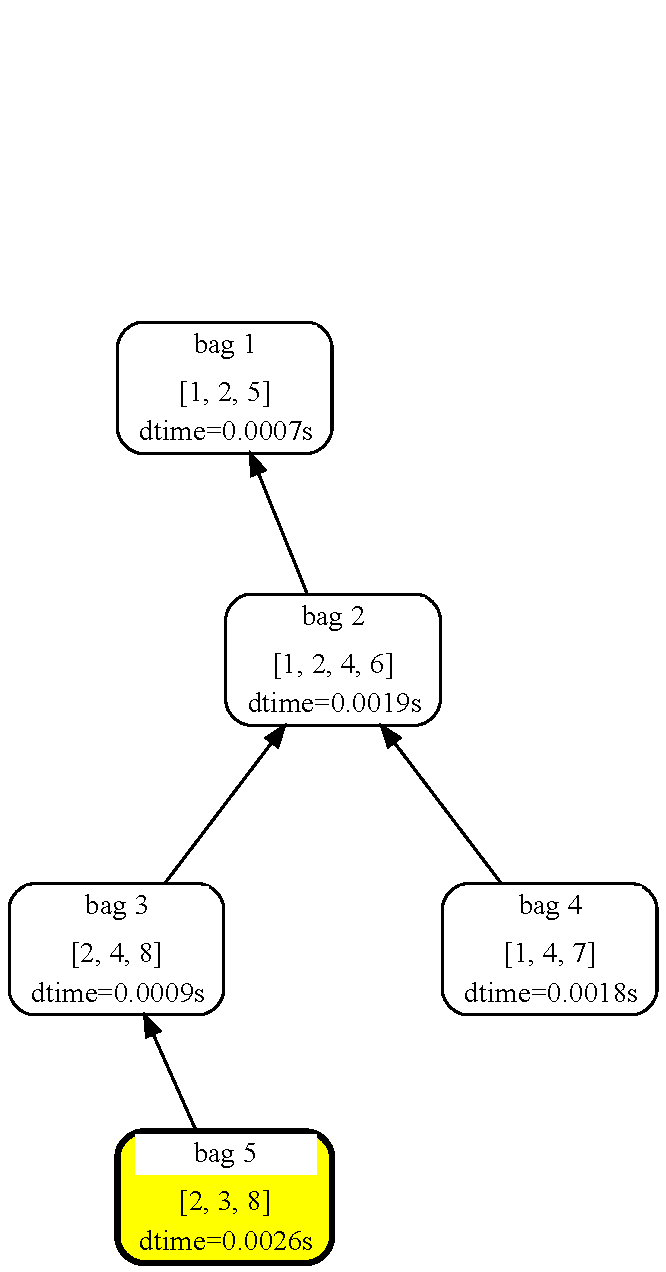
\includegraphics[height=0.6\textheight]{images/DA4SAT/results/TDStep1.pdf}
	\caption{Tree decomposition for solving example \ref{ex:example41} . \\
		With yellow highlighting for the first leaf (bag 5) to solve.}
\end{figure}
\begin{table}\sffamily
\begin{tabular}{l*3{c}}
	\toprule
	2 & 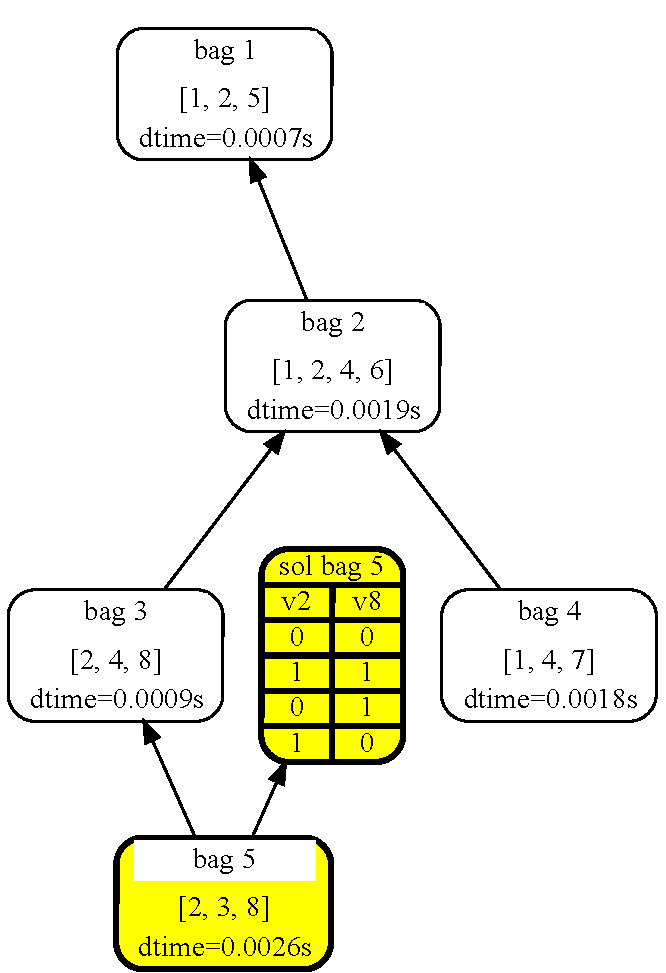
\includegraphics[height=0.46\textheight]{images/DA4SAT/results/TDStep2.pdf} &
	3 & 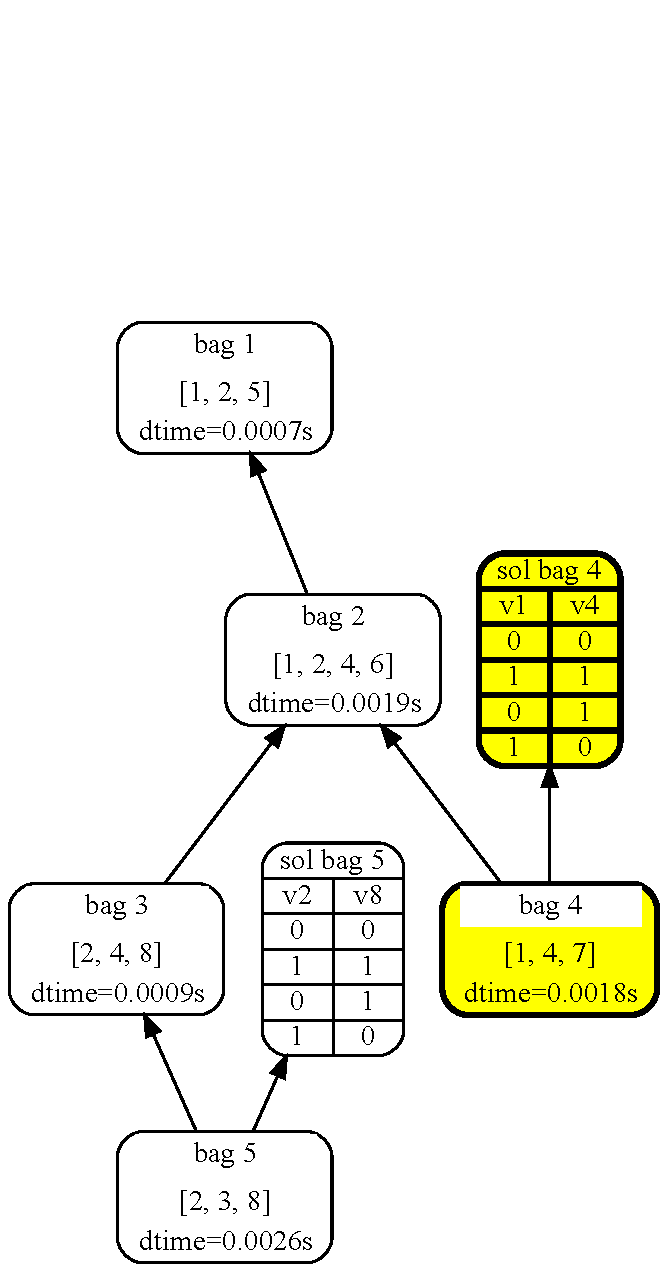
\includegraphics[height=0.46\textheight]{images/DA4SAT/results/TDStep3.pdf} \\ 
	\midrule
	4 & 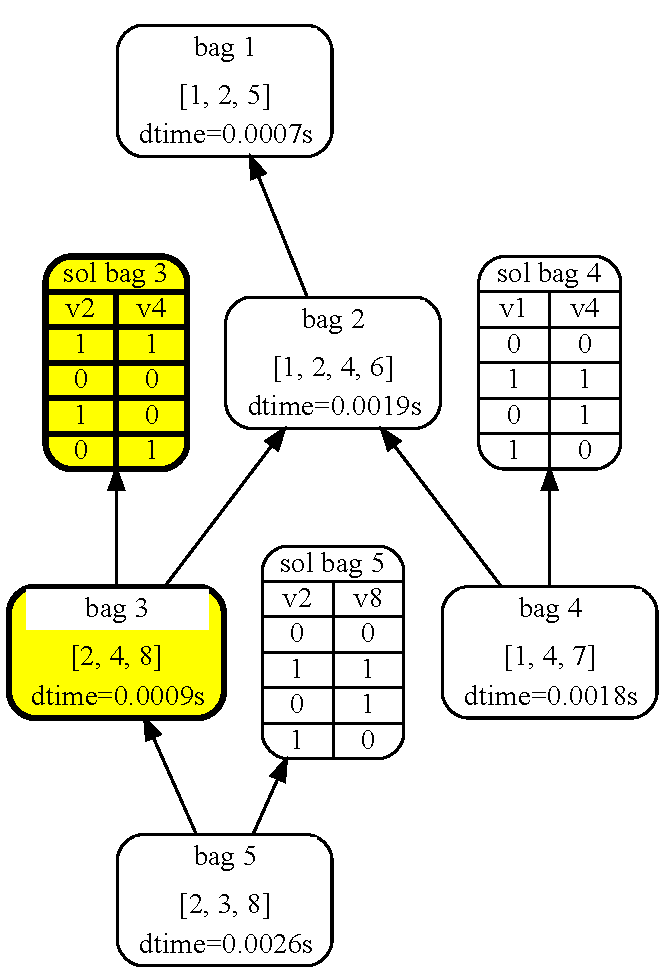
\includegraphics[height=0.46\textheight]{images/DA4SAT/results/TDStep4.pdf} &
	5 & 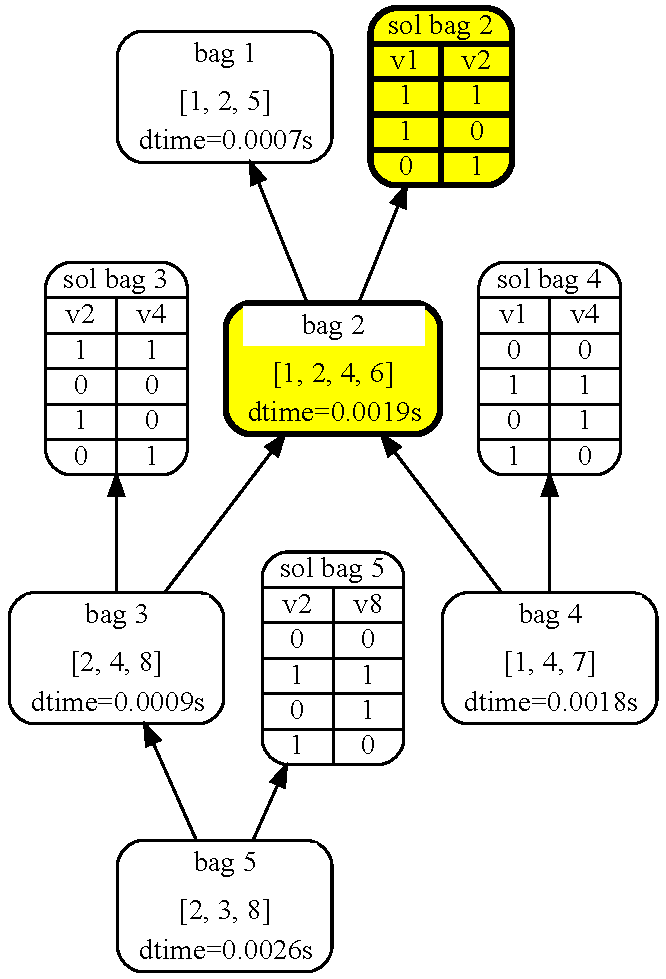
\includegraphics[height=0.46\textheight]{images/DA4SAT/results/TDStep5.pdf}\\
	\bottomrule 
\end{tabular}
\caption{Tree decomposition for solving example \ref{ex:example41} . Images for steps two to five as labeled from top left to bottom right.}
\end{table} 

\begin{figure}[H]
	\centering
	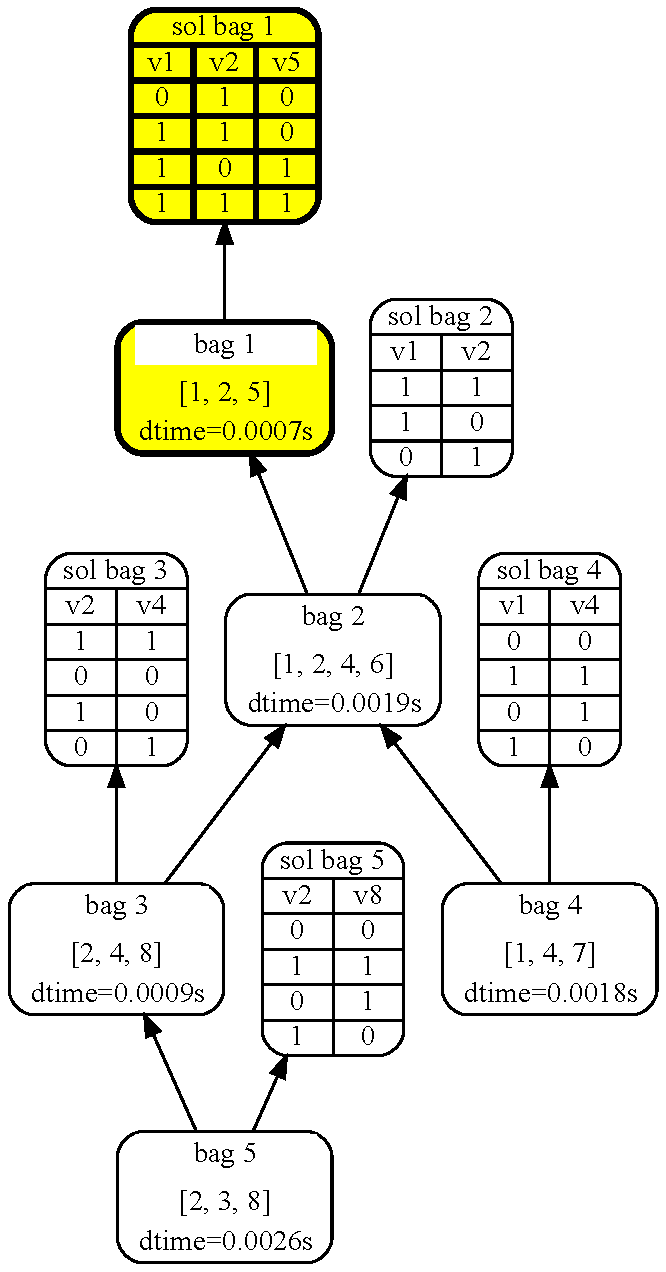
\includegraphics[height=0.6\textheight]{images/DA4SAT/results/TDStep6.pdf}
	\caption{Tree decomposition for solving example \ref{ex:example41} . \\
		Final result with yellow highlighting for the last bag (1) solved.}
\end{figure}

\begin{figure}[H]
	\setkeys{Gin}{width=\linewidth,height=0.45\textheight,keepaspectratio}
	\begin{tabularx}{\textwidth}{ l X X }
		step 1: &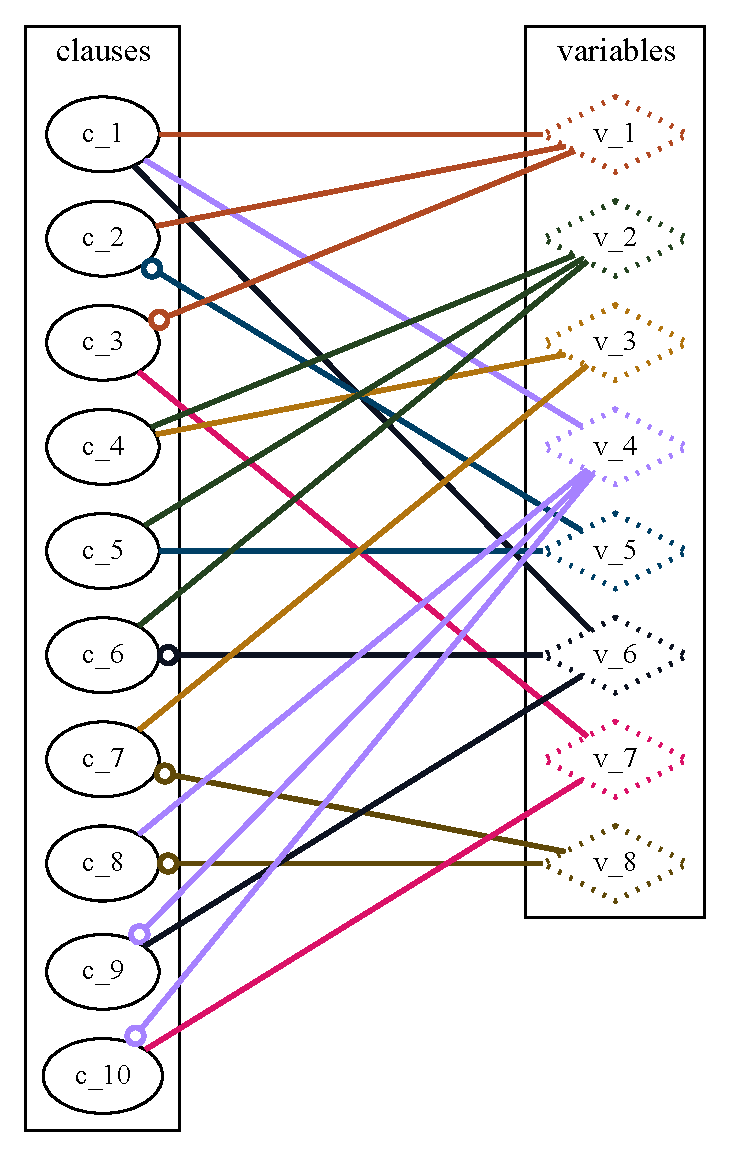
\includegraphics[valign=c]{images/DA4SAT/results/IncidenceGraphStep1.pdf} & 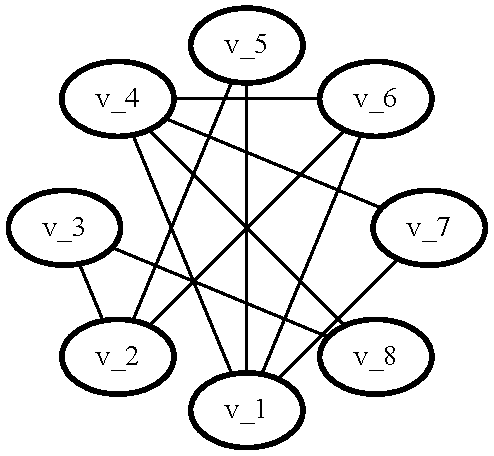
\includegraphics[valign=c]{images/DA4SAT/results/PrimalGraphStep1.pdf} \\ 
		step 2: &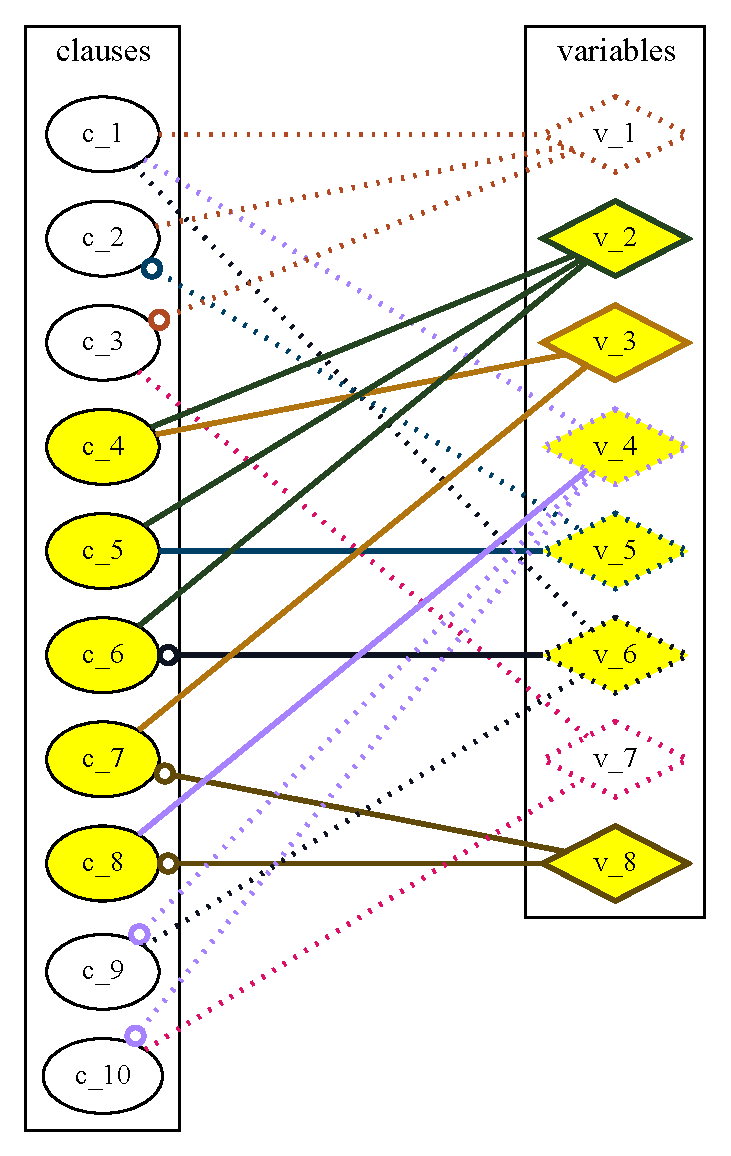
\includegraphics[valign=c]{images/DA4SAT/results/IncidenceGraphStep2.pdf} & 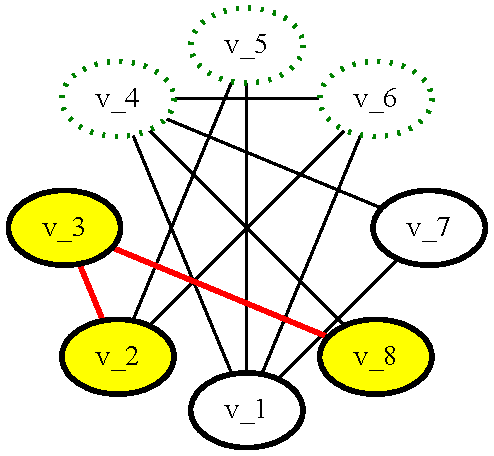
\includegraphics[valign=c]{images/DA4SAT/results/PrimalGraphStep2.pdf} \\ 
		&Visualization of the incidence graph including information for the sat formula & 
		\centering Visualization of the primal graph \\
	\end{tabularx}
	\caption{Incidence graph and primal graph of example \ref{ex:example41} .}
\end{figure}

% Appl. SharpSat
\subsection{\#SAT Example}
Like the previous example section we are interested in solutions to example \ref{ex:example41}. This time we want to solve \#SAT and count the number of solutions, that is the number of satisfying assignments. While the tree decomposition and SAT formula stay the same, we can add one column to our solution-tables compared to pure SAT solving and label this column \textit{mc} for "\textit{model-count}". We also included a footer with the API to display the sum of all models considered up to this bag.
\begin{figure}[H]
	\centering
	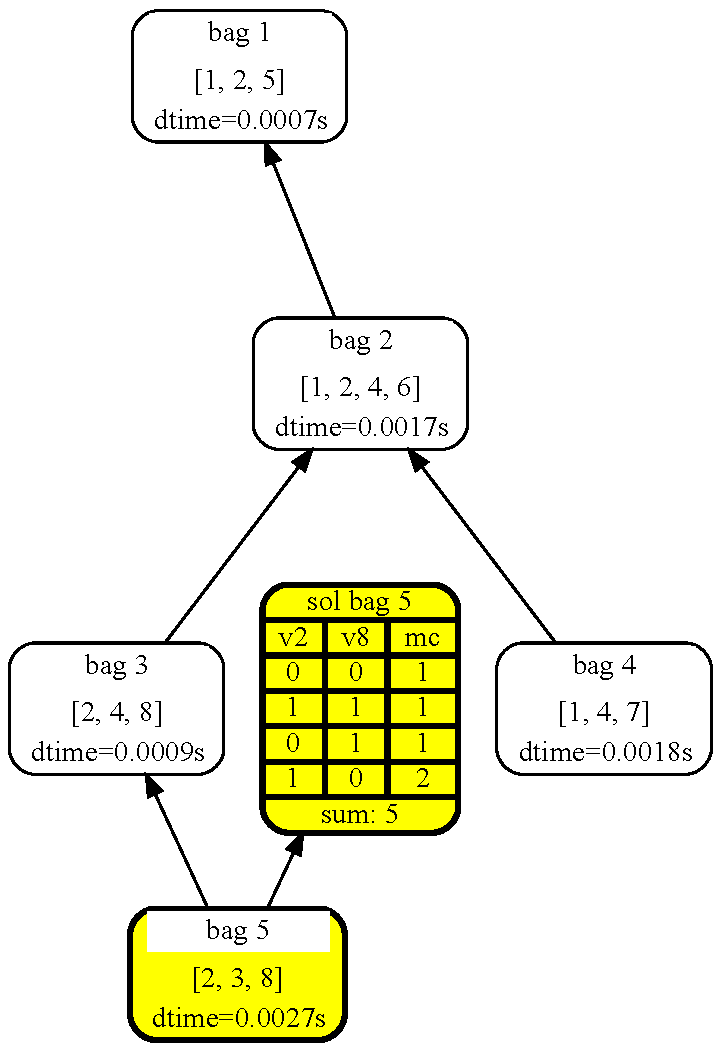
\includegraphics[height=0.6\textheight]{images/DA4/TDStep2.pdf}
	\caption{Tree decomposition for solving example \ref{ex:example41} with yellow highlighting of the solution for the first leaf.}
\end{figure}
\begin{figure}[H]
	\centering
	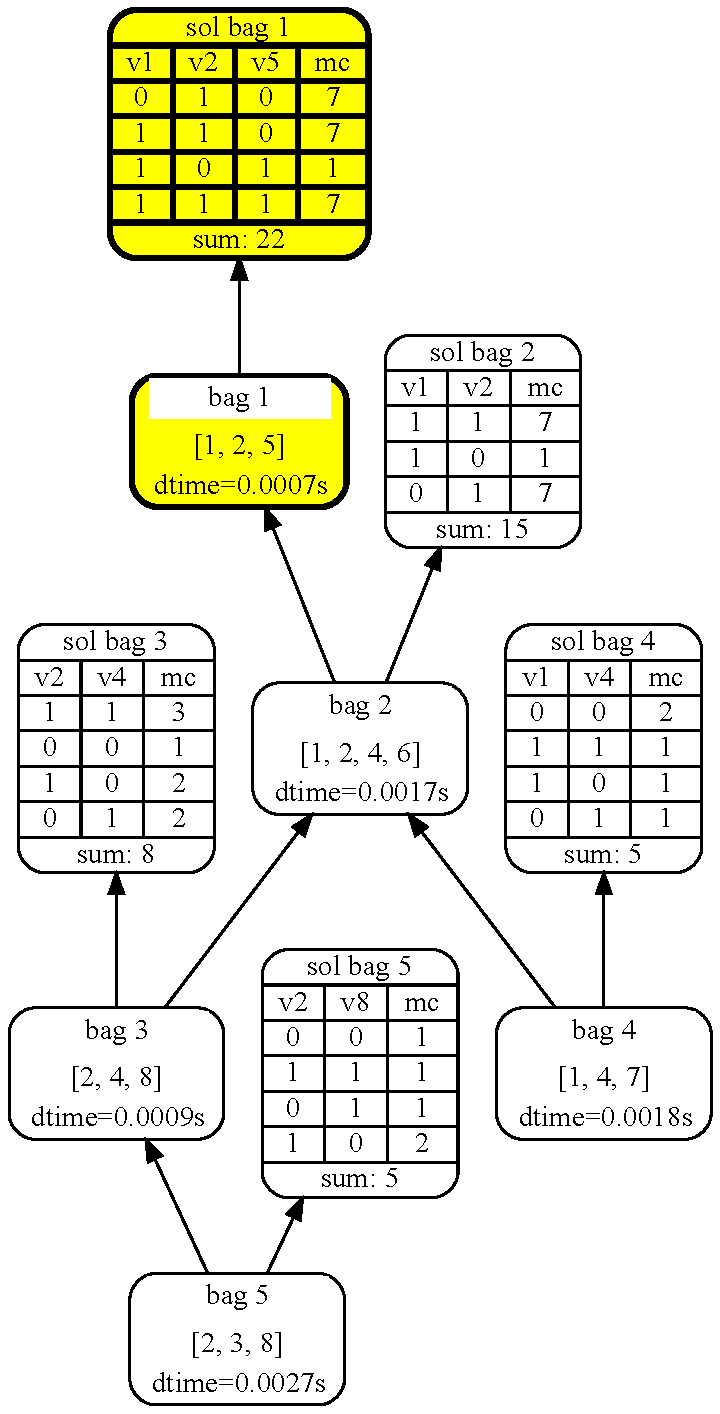
\includegraphics[height=0.9\textheight]{images/DA4/TDStep6.pdf}
	\caption{Tree decomposition for solving example \ref{ex:example41}. The highlighted bag 1 points to the solution of the problem, containing 22 solutions and satisfying variable assignments for $v_{1},v_{2},v_{5}$ contained in \textit{sol bag 1}.}
\end{figure}
% Appl. VC
\subsection{Vertex Cover Example}\label{sec:minvc}

Here we take a look at a problem that is itself formulated directly on a graph.\\
%
%Vertex Cover Problem: For a given input graph $G=(V,E)$, a \textit{vertex cover} is a set $C$ of vertices $C \subseteq V$ so that we have $\{u,v\} \cap C \neq \emptyset$ for each edge $\{u,v\}\in E$. The problem \textit{minimal vertex cover} asks to find the minimum cardinality among all vertex covers, i.e. $|C|$ is such that there is no vertex cover $C'$ with $|C'| < |C|$.

%An instance $G=(V,E)$ of \textit{minimal vertex cover} parameterized by treewidth \textit{tw} can be solved in time $\mathcal{O}(2^{tw(G)}|V|)$ \cite{HenningParamAlgo}.

For details on the algorithms used by the solvers see also \cite[Ch. 4.2]{dpdbpadl2020} on MinVC and its Listing 3 for a template for general problems.

As a very small example we will try to solve \textit{minimal vertex cover} for the following graph in Figure \ref{fig:wheelgraph} with edges seen in listing \ref{lst:wheelgraph}.

\begin{figure}[H]
	\centering
	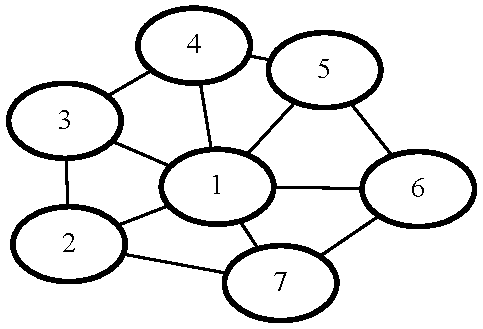
\includegraphics[]{images/WheelGraph7/graph1.pdf}
	\caption{Wheel graph with 7 vertices.}
	\label{fig:wheelgraph}
\end{figure}


\begin{figure}[H]
	\centering
		First step solving \textbf{bag 2}
	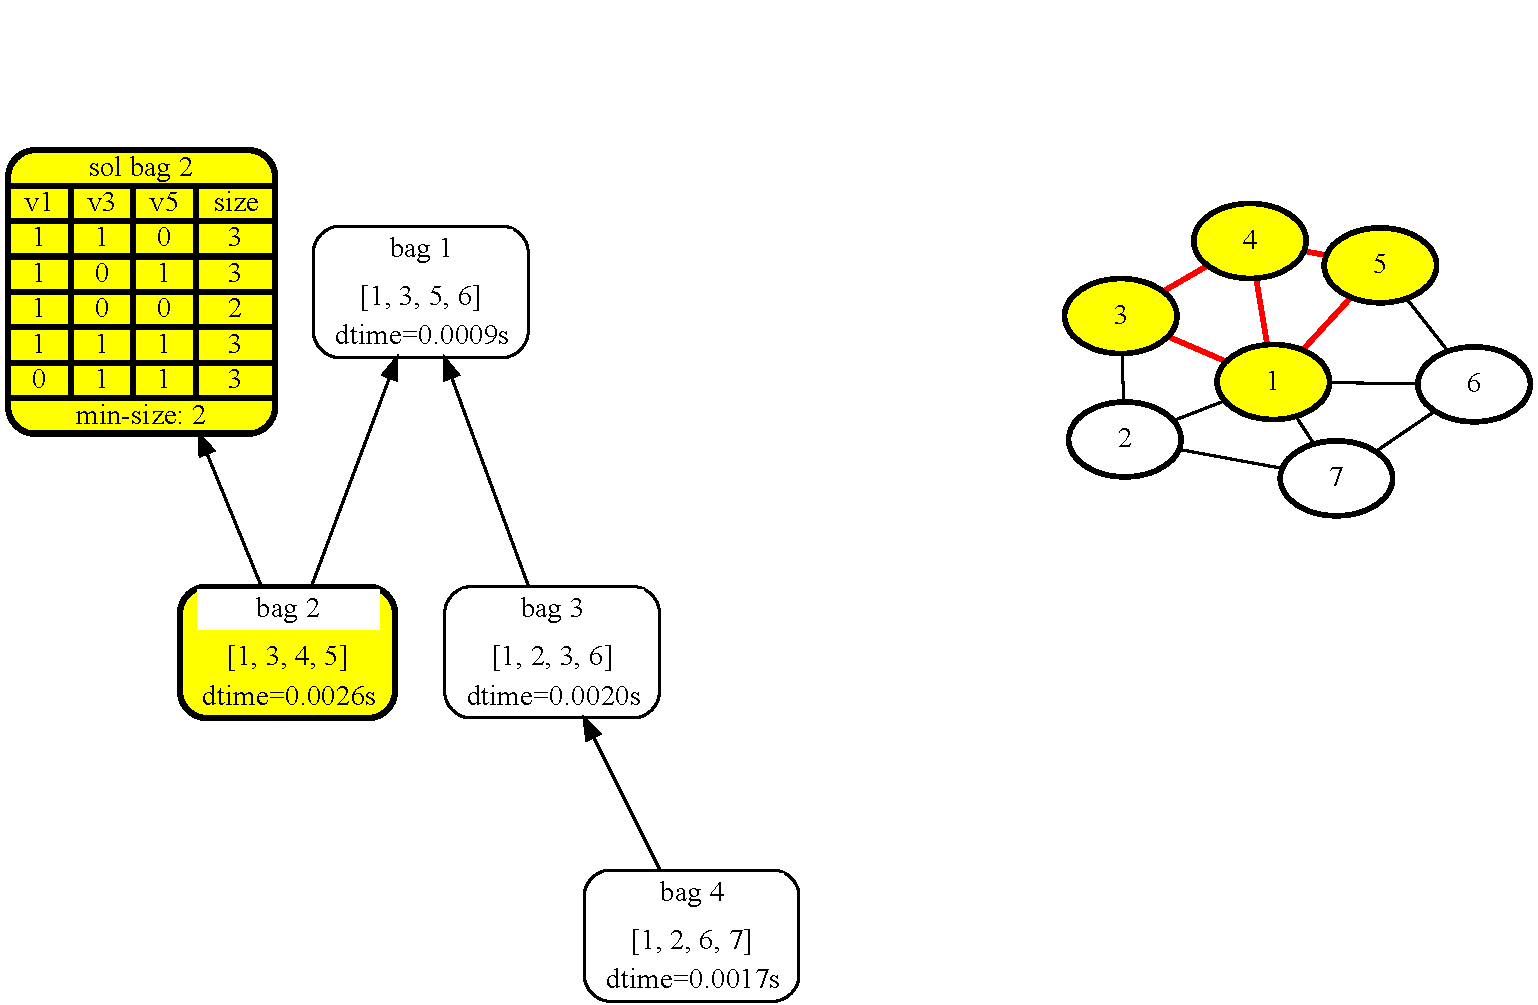
\includegraphics[width=0.9\linewidth]{images/WheelGraph7/combined2.pdf} \vspace{1em}\\
	Second step solving \textbf{bag 4}\\
	
		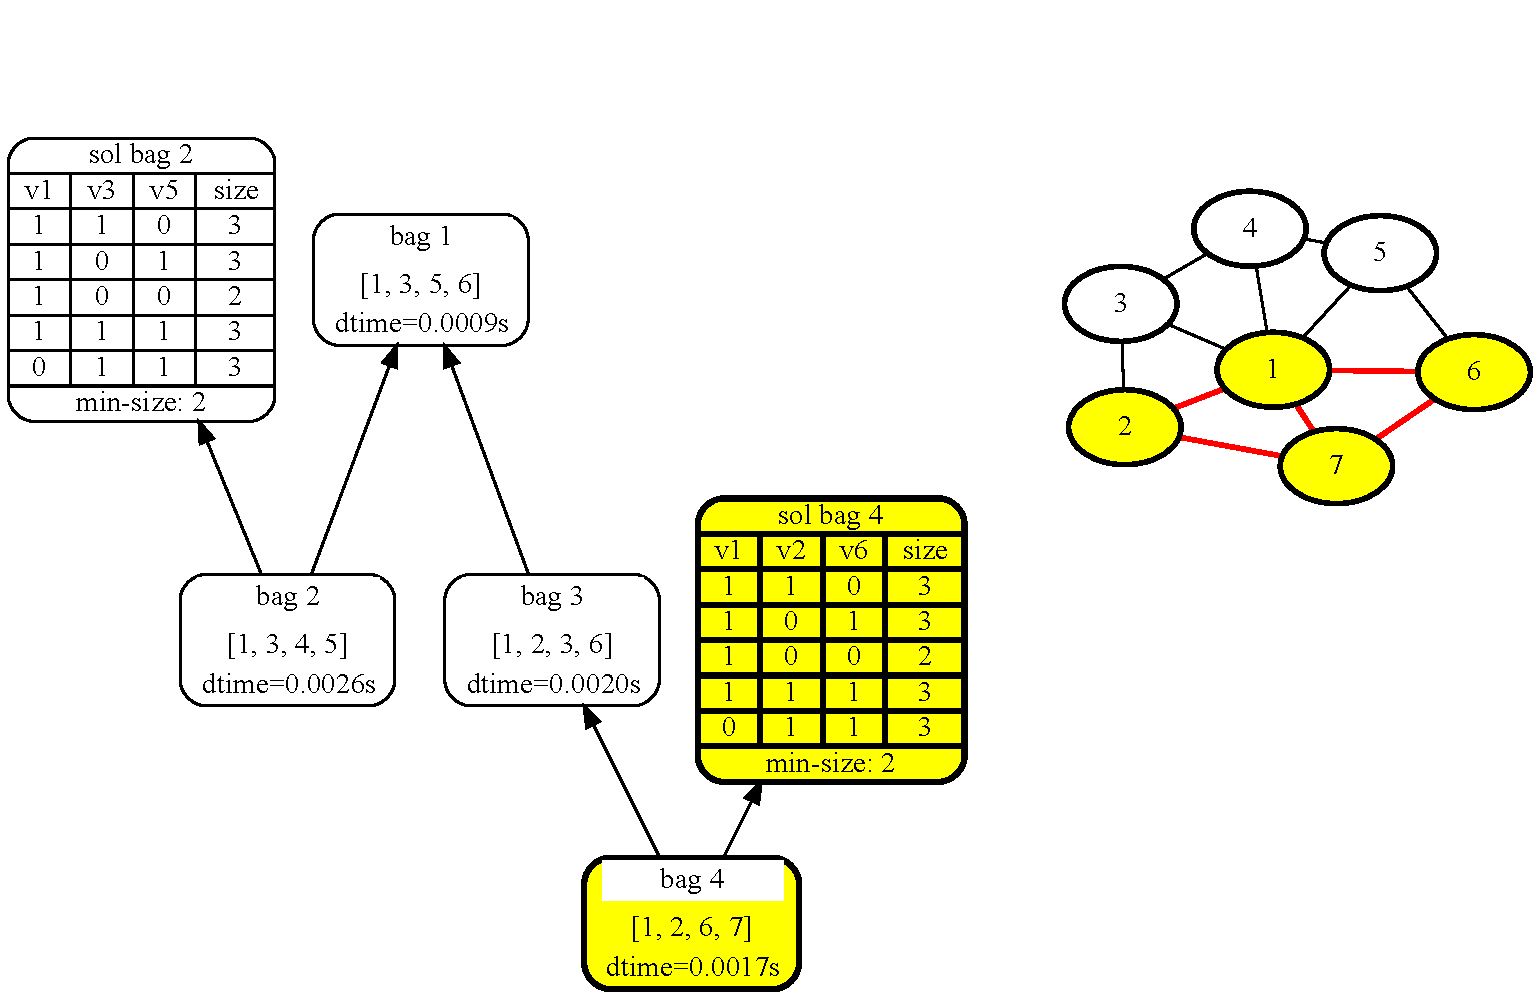
\includegraphics[width=0.9\linewidth]{images/WheelGraph7/combined3.pdf}
	\caption{First steps to solve \textit{minimal vertex cover} for example graph \ref{fig:wheelgraph} on it's tree decomposition.}
	\label{fig:wheelgraphc23}
\end{figure}
\begin{figure}[H]
	\centering
	Third step solving \textbf{bag 3} \vspace{1em}\\
	
	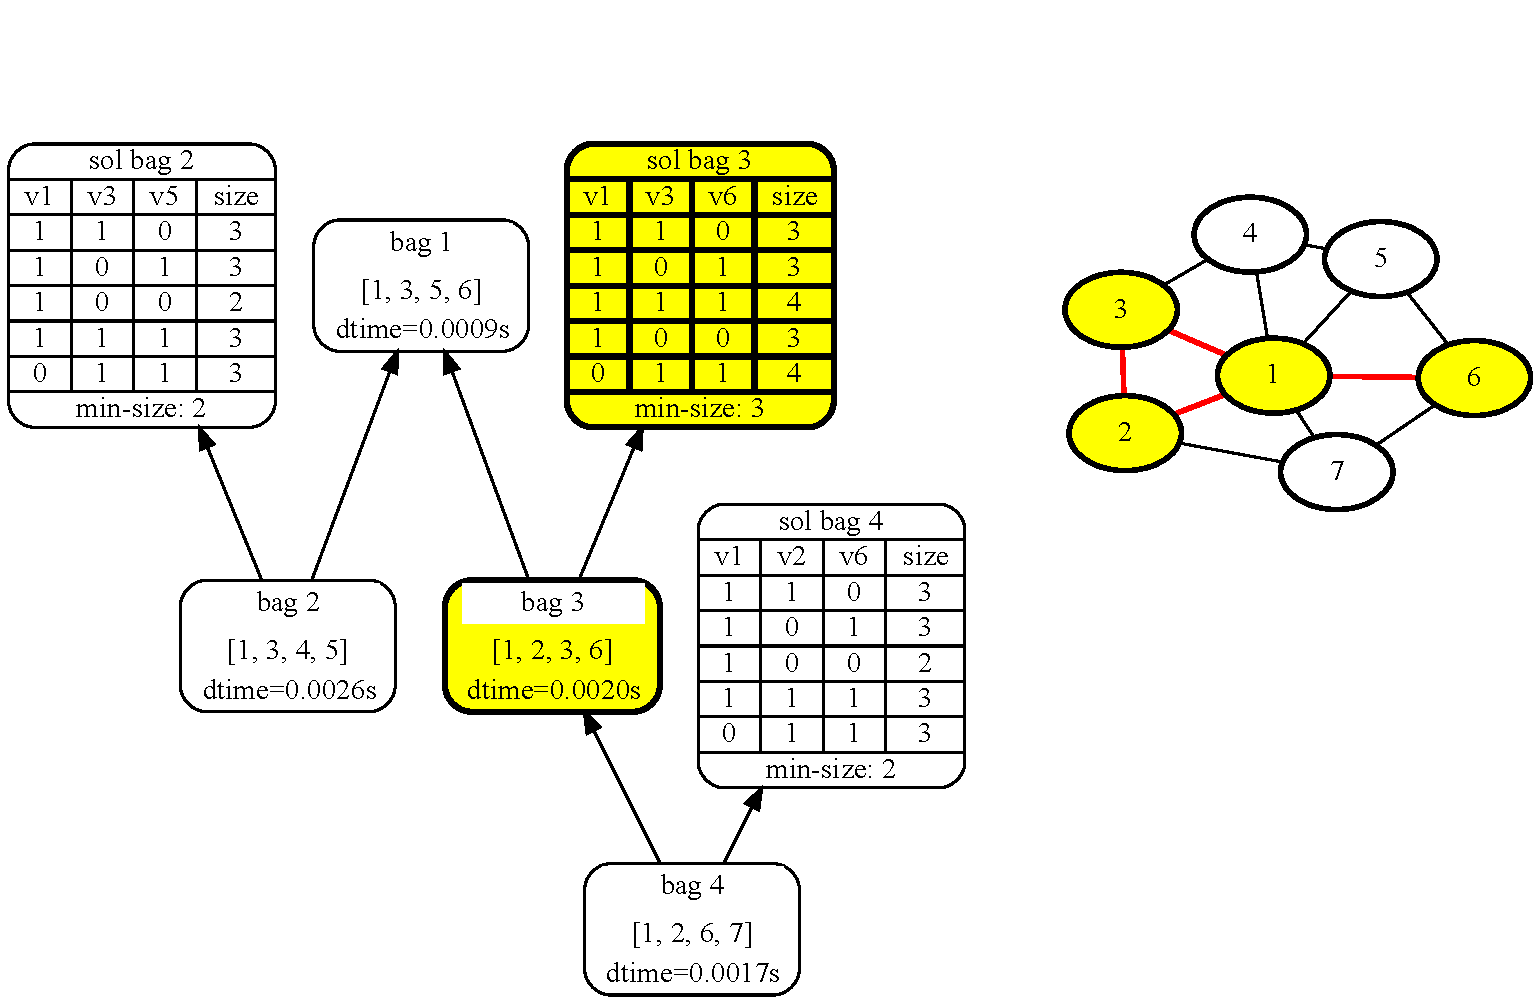
\includegraphics[width=0.9\linewidth]{images/WheelGraph7/combined4.pdf}\\
	\vspace{0.5em}
	Fourth step solving \textbf{bag 1}\\
	
	\vspace{0.6em}
	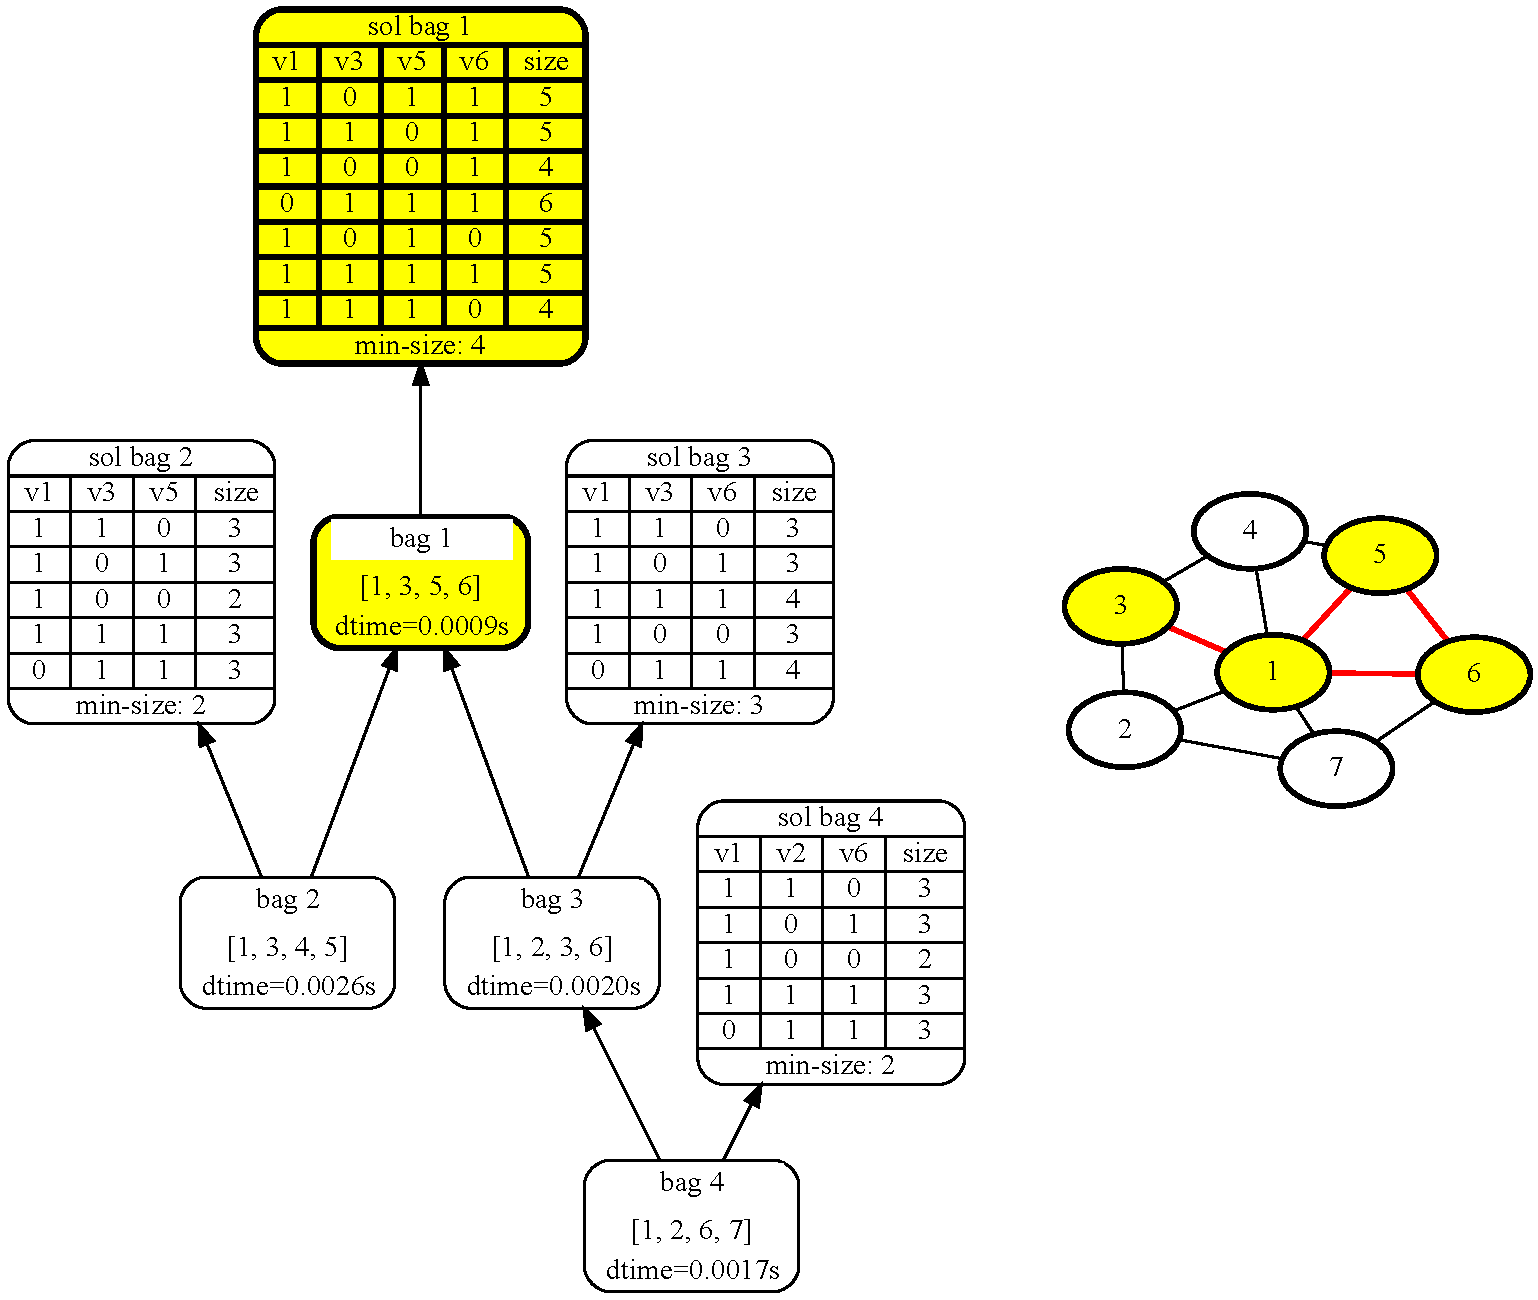
\includegraphics[width=0.9\linewidth]{images/WheelGraph7/combined5.pdf}\\
	
	\caption{Last steps to solve \textit{minimal vertex cover} for example graph \ref{fig:wheelgraph} on it's tree decomposition.}
	\label{fig:wheelgraphc45}
\end{figure}


% Appl. svgjoin with different options
\subsection{SVG Join Example}

After creating several images at each visualization step all images from this step can be automatically combined into one SVG. In this chapter we expand on Section \ref{sec:svgjoin} with some practical applications of this concept.

With the four parameters \textit{centerpad}, \textit{v\_bottom}, \textit{v\_top} and \textit{scale2} we can specify the order in which images will be placed next to each other. To explain some configurations we will take the generated images from the previous chapter.

In Figure \ref{fig:joindefault} the two images are joined with default values for all parameters, in order (\textit{TDStep, graph}). 

As we can see the solutions for bags other than 2 are hidden in the output but are taken into account in the image size. The right graph is aligned to the upper edge of the left image. With no padding between the images \textit{graph} image is attached to the right edge of the first image visualizing the {tree decomposition}.

\begin{figure}[H]
	\centering
	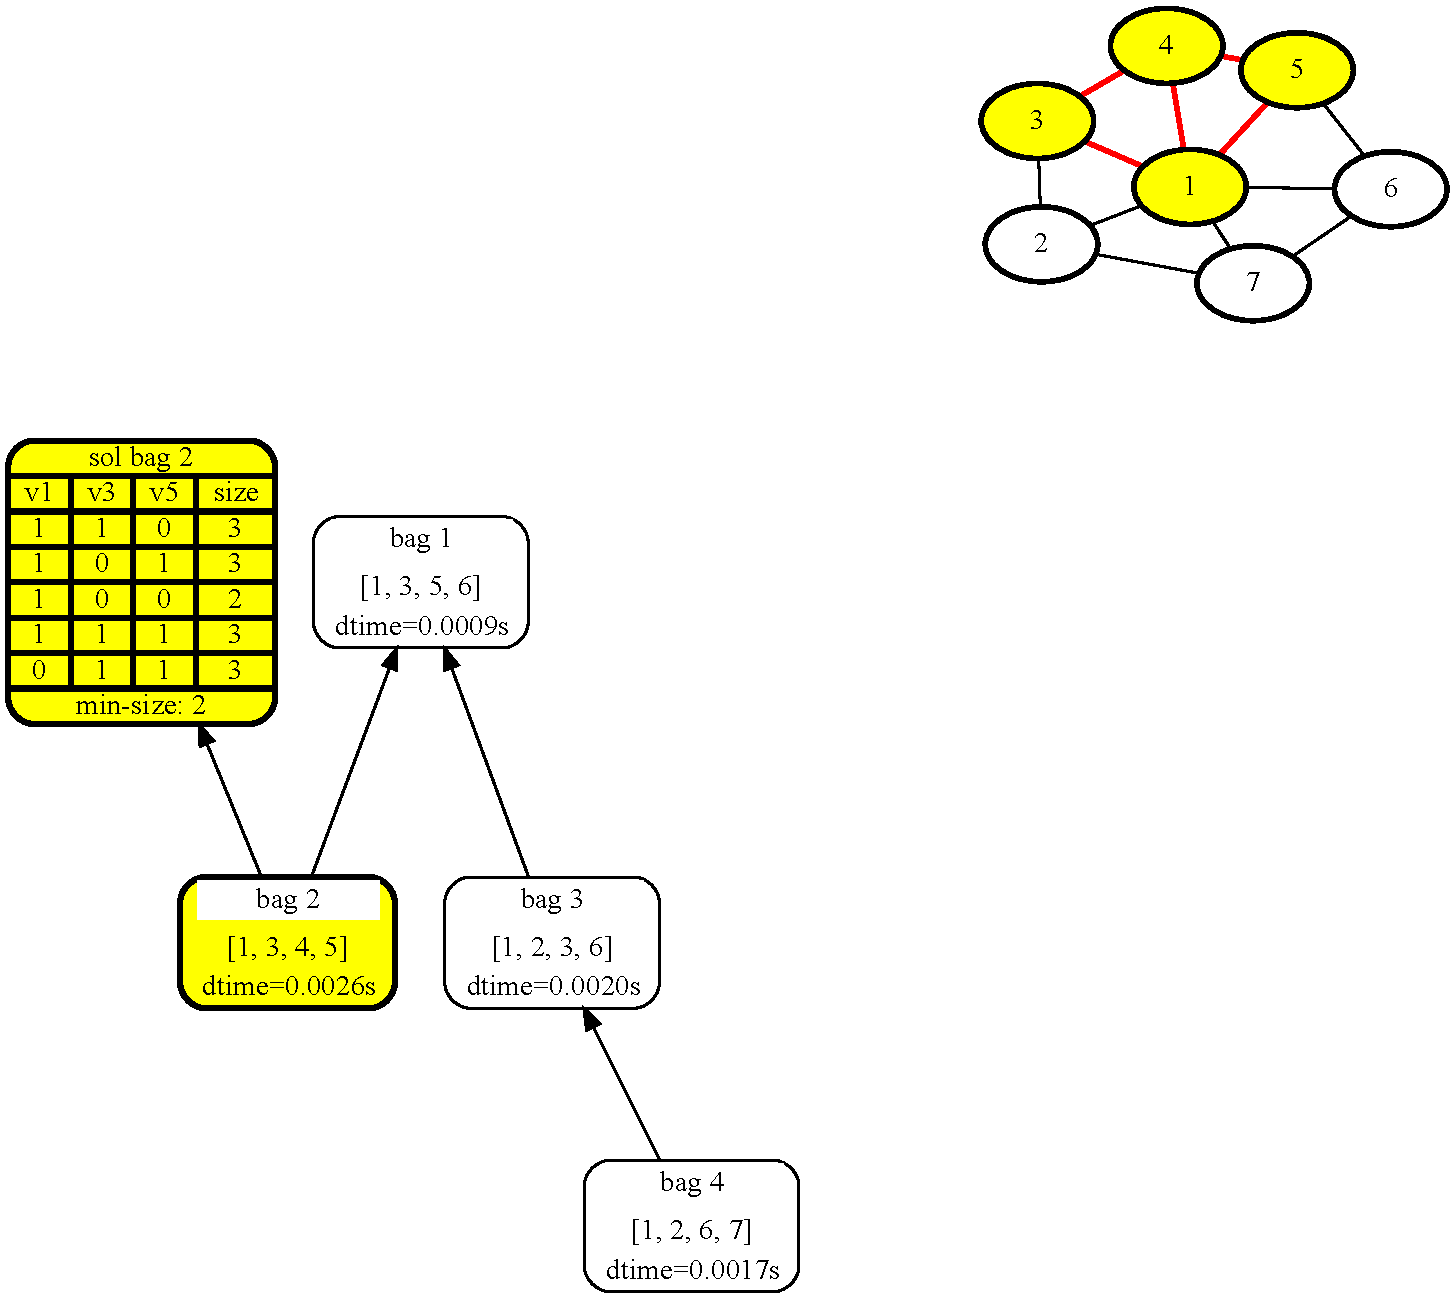
\includegraphics[width=\linewidth,height=0.6\textheight,keepaspectratio]{images/SVGJOIN/default2.pdf}
	\caption{Joining results from Section \ref{sec:minvc} with default parameters at step 2.}
	\label{fig:joindefault}
\end{figure}
%svg_join(['TDStep', 'graph'],
%'Archive/WheelGraph7',
%outname="default_06",
%padding=[0,0,0,40],
%v_bottom=0.6,
%num_images=5)
\begin{figure}[H]
	\centering
	\textbf{v\_bottom = ``bottom"} \vspace{1em}\\
	
	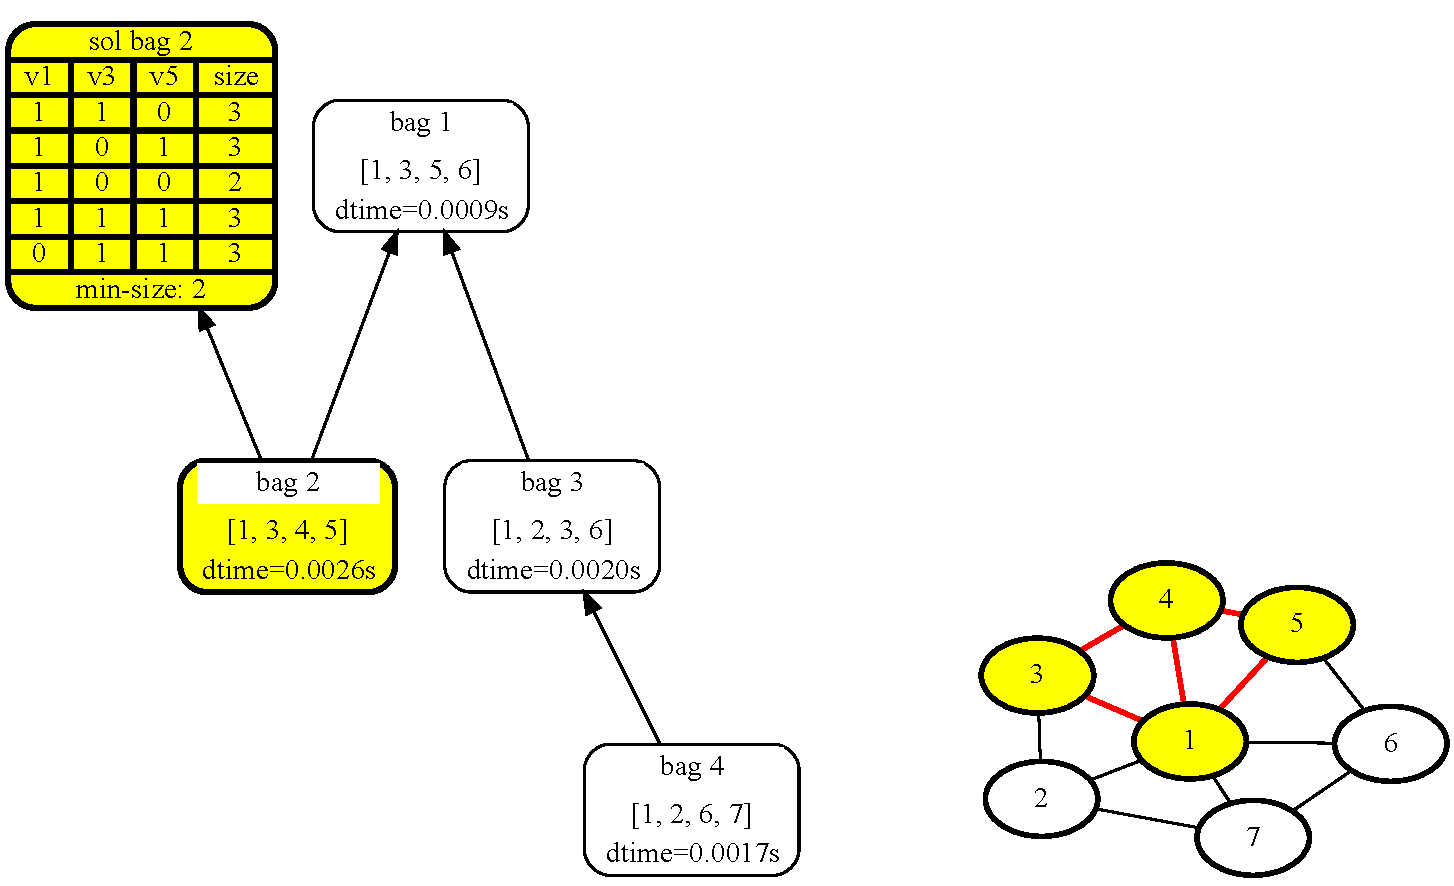
\includegraphics[width=\linewidth]{images/SVGJOIN/default_bottom2.pdf}\\
	\vspace{0.5em}
	\textbf{v\_bottom = ``center"}\\
	
	\vspace{0.6em}
	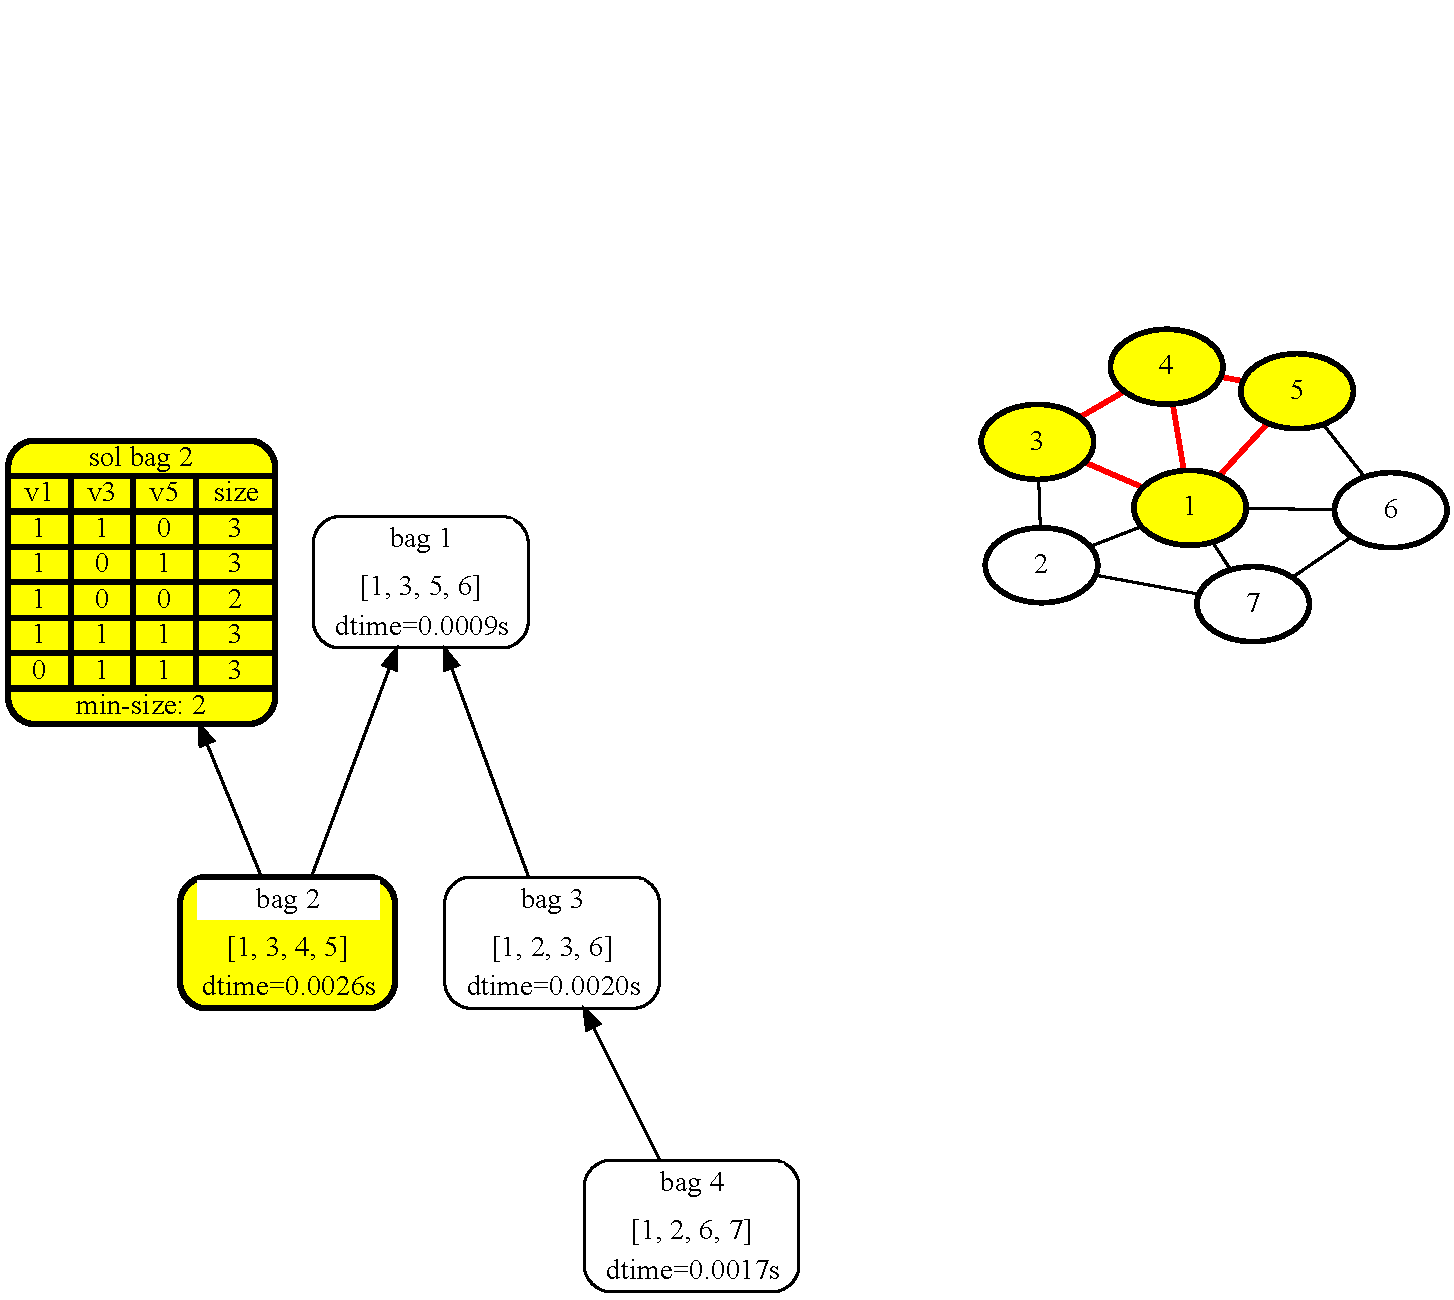
\includegraphics[width=0.9\linewidth]{images/SVGJOIN/default_center2.pdf}
	\caption{Joining results from Section \ref{sec:minvc} at step 2 and setting v\_bottom. The invisible (empty) parts of the graphics is cropped from the top of each.}
	\label{fig:joinbotcenter}
\end{figure}
\begin{figure}[H]
	\centering
	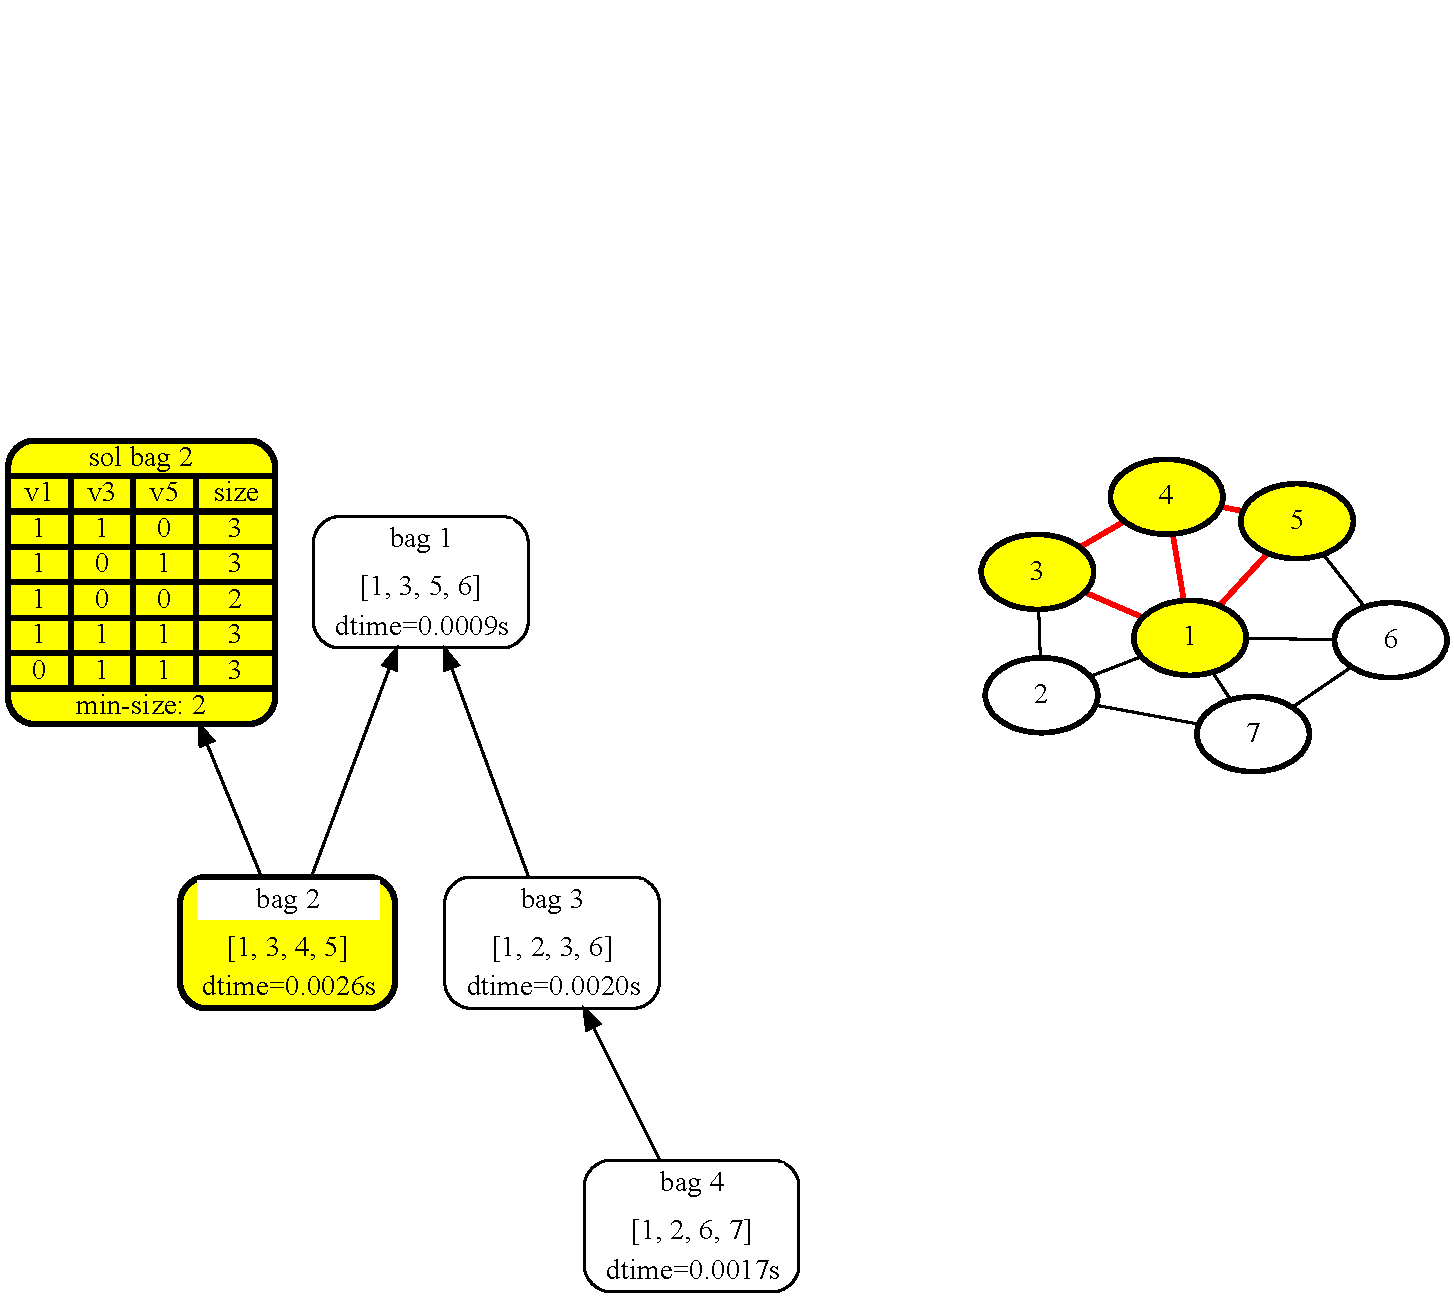
\includegraphics[width=0.9\linewidth,height=0.9\textheight,keepaspectratio]{images/SVGJOIN/default_062.pdf}
	\caption{Joining results from Section \ref{sec:minvc} at step 2 and shifting bottom edge of second image to $60\%$ height of the first image.}
	\label{fig:join60}
\end{figure}

In Figure \ref{fig:joinbotcenter} the parameter v\_bottom is set to ``bottom" to align both graphics on the bottom edge; set to ``center" elevates the right image to 50\% of the height of the first. It is also possible to provide arbitraty floating-point values for vertical adjustment as presented in Figure \ref{fig:join60} with v\_bottom = 0.6 .\\
\\
if we want the right graphic a bit larger compared to the default size, we can add additional scaling by providing the argument \textbf{scale2}. In figures \ref{fig:joinscaled1} to \ref{fig:joinscaled5} the complete time series for solving \textit{minimal vertex cover} for example \ref{lst:wheelgraph} with join-parameters
\begin{itemize}
	\item[] padding = [0, 0, 0, 40]
	\item[] v\_bottom = 0.6,
	\item[] scale2 = 1.5
\end{itemize}
can be seen. \\
To further visualize the progress of the algorithm in the results one could use the possibility to specify multiple values for all the transformation parameters \textit{centerpad}, \textit{v\_bottom}, \textit{v\_top} and \textit{scale2} and elevate the second image with the values for\\
 v\_bottom = [1, 0.85, 0.7, 0.55, 0.4]. \\
 This is done in figures \ref{fig:joinscaledrise1} to \ref{fig:joinscaledrise5}.

% Finding a bug using visualization
\subsection{Visualization of Defects}
 
As stated in the introduction, most of the data we visualize is already present in the solvers.
Given the right testing frameworks it is possible to produce a report for structural or even randomly occurring defects in the solver. As the software we used for our experimental visualizations shown in this work does not itself contain a test environment, we were able to reproduce some undiscovered ``bugs" using and developing our visualization tool.


 One specific program invocation did not give the expected result solving a \textit{vertex cover} with one hundred nodes. The problem was first found when inspecting the immediate output of the program \textit{dpdb.py}, which did report the wrong result size. The problem could be localized in the tree decomposition, leading to the whole result table being pruned - see the visualization in Figure \ref{fig:starsbag59}. It is obvious that ``bag 59" is disconnected from its parent ``bag 57", even if its nodes occurred in other bags in the tree. This violates our rule $3$ of the TD (``the set of bags that contain the variable v induce a connected sub-graph of T.").  This particular bug occurred only with a specific seed and on the windows operating system. 

\begin{figure}[H]
	\centering
	\vspace{1em}
	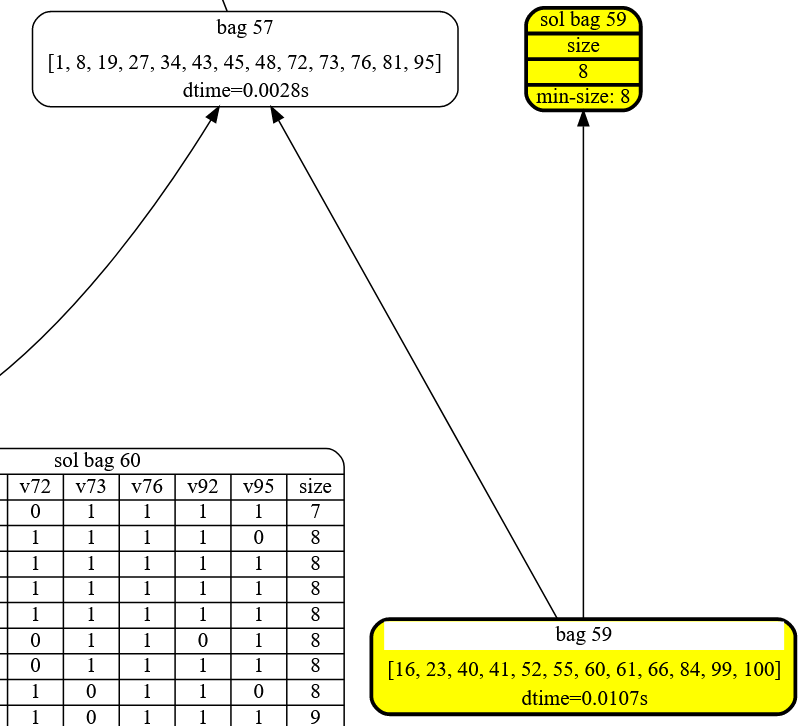
\includegraphics[width=0.9\linewidth,height=0.9\textheight,keepaspectratio
					]{images/starsbag59.png}
		\vspace{1em}
	\caption{Part of interest to find a problem with bag 59 in visualization. }
	\label{fig:starsbag59}
\end{figure}

%\begin{figure}[H]
%	\centering
%	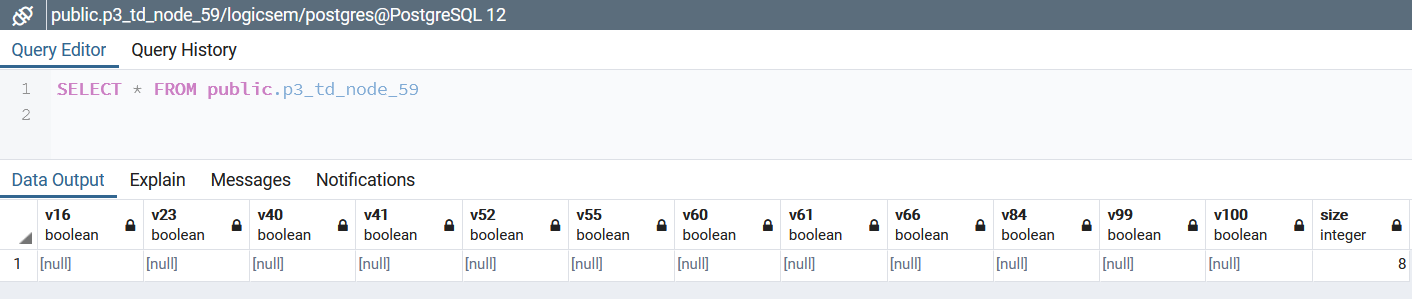
\includegraphics[width=0.9\linewidth,height=0.9\textheight,keepaspectratio]{images/Found bag 59 in stars100 with seed0.png}
%	\caption{Bag 59 in the database table.}
%	\label{fig:bag59visu}
%\end{figure}

The problem was located in the version of \url{https://github.com/TU-Wien-DBAI/htd} used to create the tree decomposition, which in this instance and for the seed $0$ did not place bag 59 in the right place in the tree-decomposition on our Windows 10 machine. We can see the bags of the tree decomposition in Figure \ref{fig:bag59td}, where the bags containing variable 100 are indicated in red. 

\begin{figure}
	\centering
	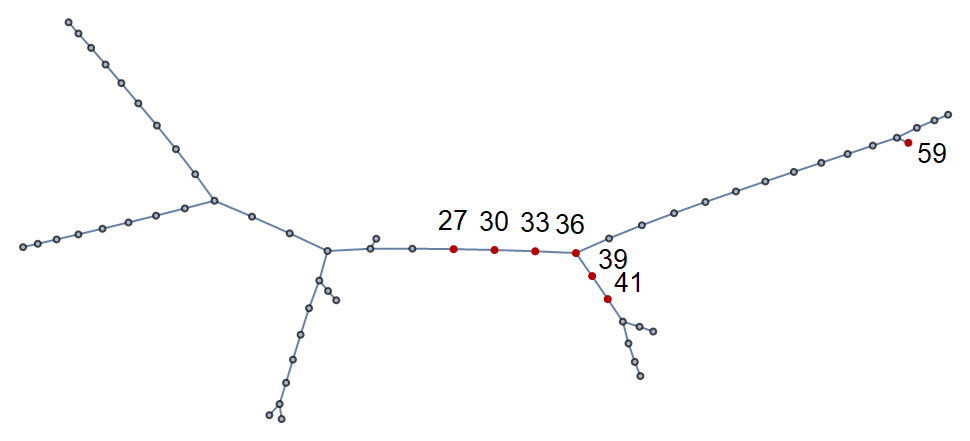
\includegraphics[width=0.9\linewidth,height=0.9\textheight,keepaspectratio]{images/stars100var100.png}
	\caption{Bag 59 can be seen on the far right of the graphic.}
	\label{fig:bag59td}
\end{figure}
%==============================================================================
%============== Conclusion ====================================================
%==============================================================================
\newpage
\section{Conclusion}\label{sec:conclusion}
%What is achieved?
% Open source Assistant for visualizing dynamic programming on tree decompositions
% Small dataformat, highly adaptable svg format
% Two example integrations in actively developed MSO solvers
% Bags do provide the option to add arbitrary many/long labels for different debugging information
\subsection{Summary}
We created a program which can automate the visualization of dynamic programming on tree decompositions. All tree decomposition nodes are prepared to display multiple user-defined strings, which can contain various debugging information about the run.
With SVG we support by default a fast and easily editable image format.\\

The visualization is implemented in two actively developed solvers for the problem types {SAT}, {\#SAT} and {minimal vertex cover}. We have tested the visualization of each problem type with graphs of different sizes - with nodes in the order of $10^{0..2}$ for MinVC and $10^{0..3}$ for SAT and \#SAT.

During the development we could already find some bugs in the solvers.

We have defined a data exchange API to give the visualization the information it needs and provided meaningful default values for most parameters. The API supports the interchange of:
\begin{itemize}
	\item One tree decomposition
	\item Time steps that add solutions to the TD
	\item Incidence graphs for problems on boolean formulas, from which primal and dual graphs can be created automatically
	\item Simple graphs for general graph problems
	\item The merging of several visualizations of a time step into one image
\end{itemize}


\subsection{Future Work}
% Graphs could provide more options to the user
% Generate multiple bipartite and general graphs
% Operate on hypergraphs
% Bring all timesteps into one file, e.g Animations
In the future our graphs could provide even more parameters to the user. \\

Different colors visualizing attributes of each node are a consideration.\\

Show path of various solutions from leaf to bag. \\

The next step would be to expand the API to multiple bipartite or simple graphs, which right now is limited to one each with the option to create primal- and dual-graphs too.\\

One addition would be the inclusion of hypergraphs (graphs where one edge does connect multiple nodes) which could be of great interest for future solvers.\\

Right now even with the \textit{svg-join} tool we need multiple files to represent all time steps. SVG however would be able to only create one file where the time steps will be animated. Animations might get toggled by the user or change over a specified time span.
%==============================================================================
%============== APPENDIX ======================================================
%==============================================================================
\newpage
\appendix
%============== Images ======================================================
\section{Images}
%\begin{figure}[H]
%	\centering
%	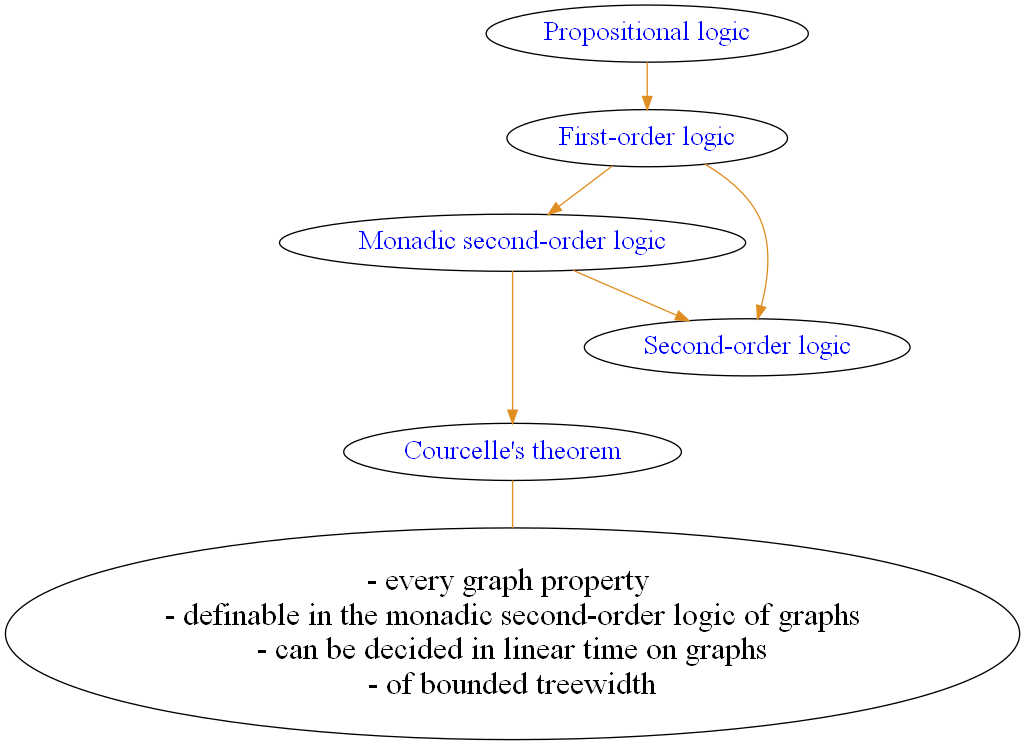
\includegraphics[width=0.8\linewidth]{images/logictheory.png}
%	\caption{From propositional logic to monadic second order logic and Courcelle's Theorem}
%	\label{fig:logictheory}
%\end{figure}
\begin{figure}
	\centering
	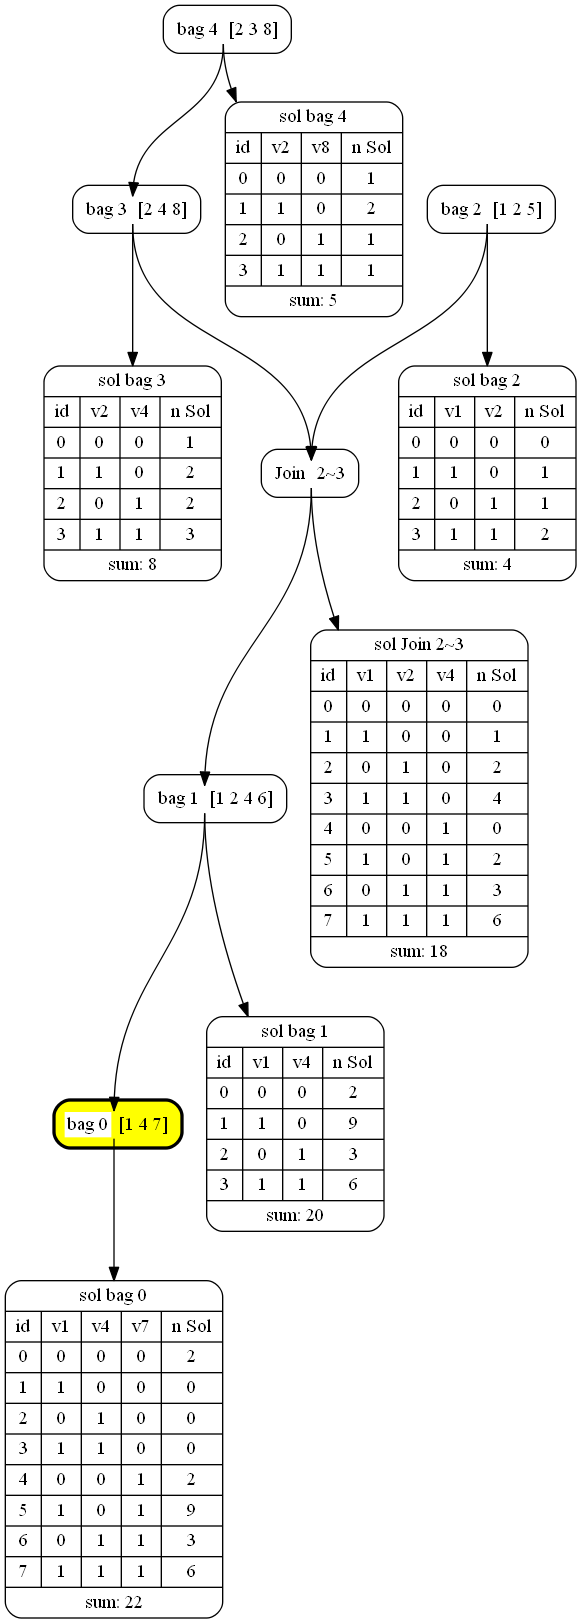
\includegraphics[height=\textheight]{images/g41digraphdot.png}
	\caption{Created scalable-vector-graphic directly from \ref{lst:g41digraphdot}}
	\label{fig:g41Digraph}
\end{figure}

%svg_join(['TDStep', 'graph'],
%'Archive/WheelGraph7',
%outname="default_06sc15",
%padding=[0,0,0,40],
%v_bottom=0.6,
%scale2=1.5,
%num_images=5)


\begin{figure}
	\centering
	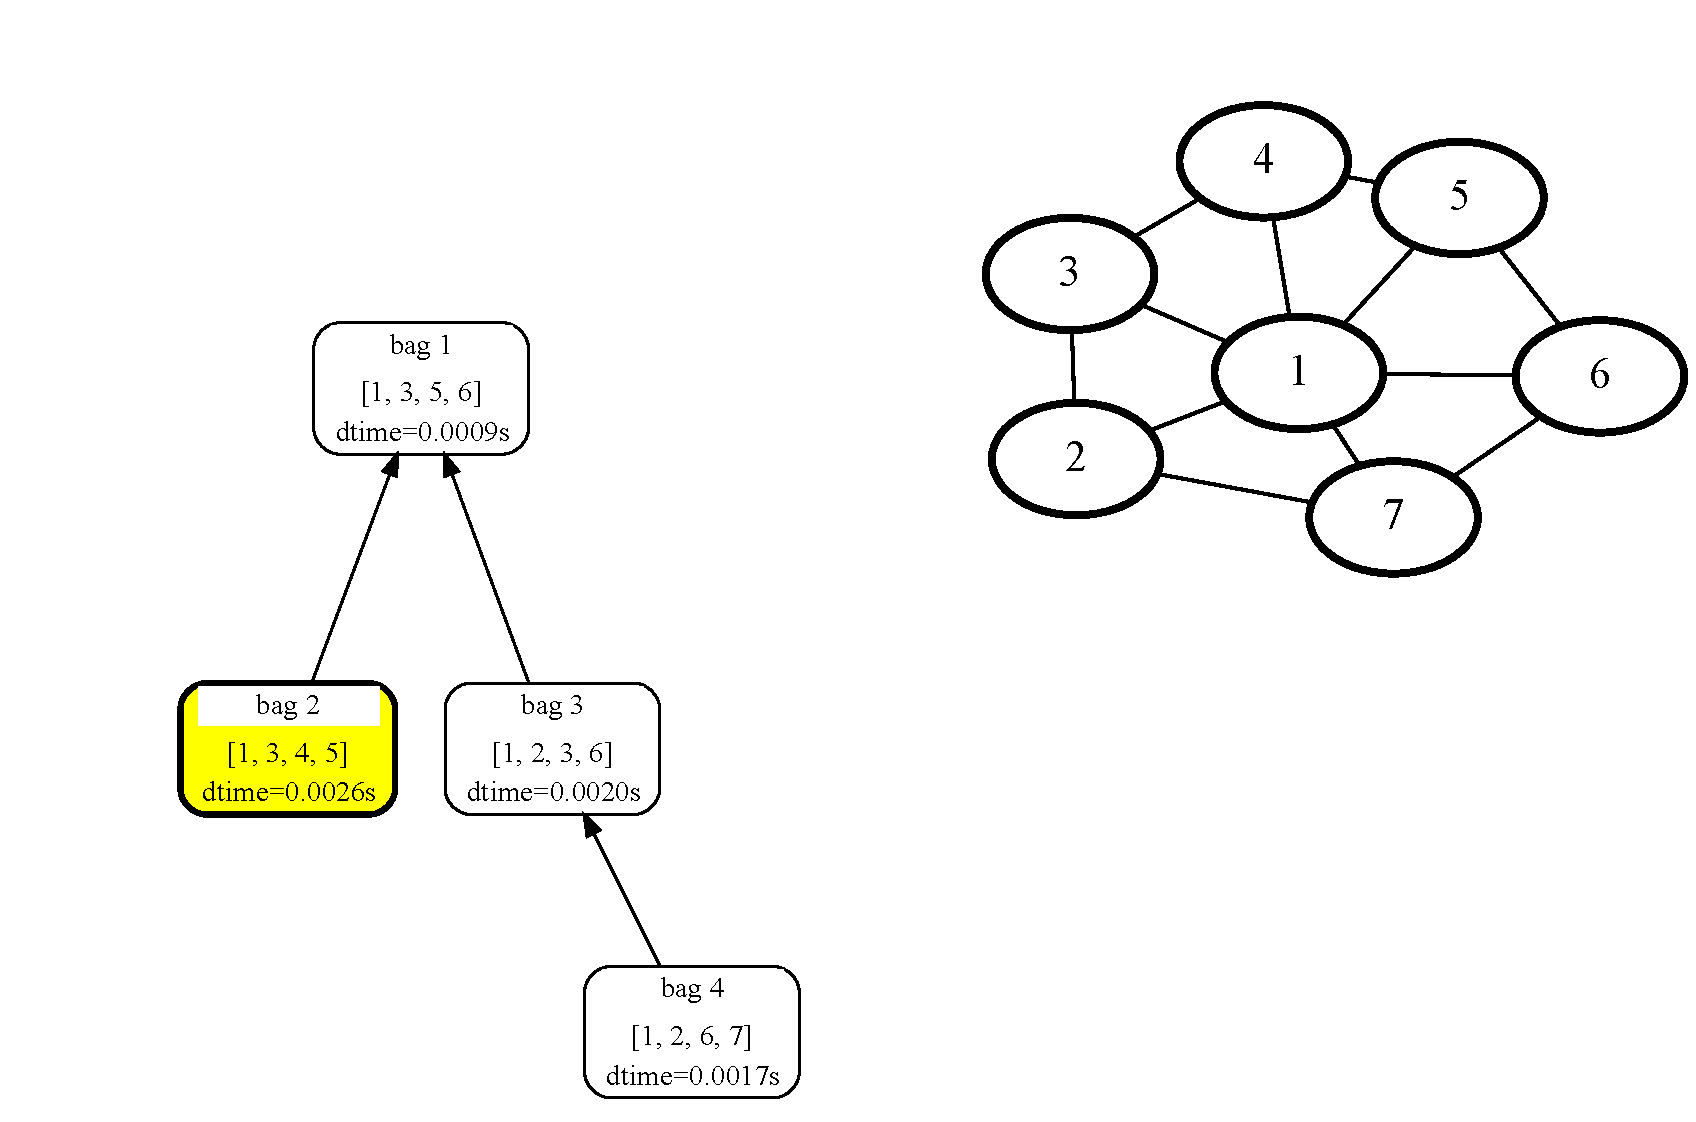
\includegraphics[width=0.9\linewidth,height=0.9\textheight,keepaspectratio]{images/SVGJOIN/default_06sc151.pdf}
	\caption{Joining results from Section \ref{sec:minvc} at step 1. Also shifting the second graphic to $40\%$ height of the first image and scaling with scale2 = 1.5 .}
	\label{fig:joinscaled1}
\end{figure}
\begin{figure}
	\centering
	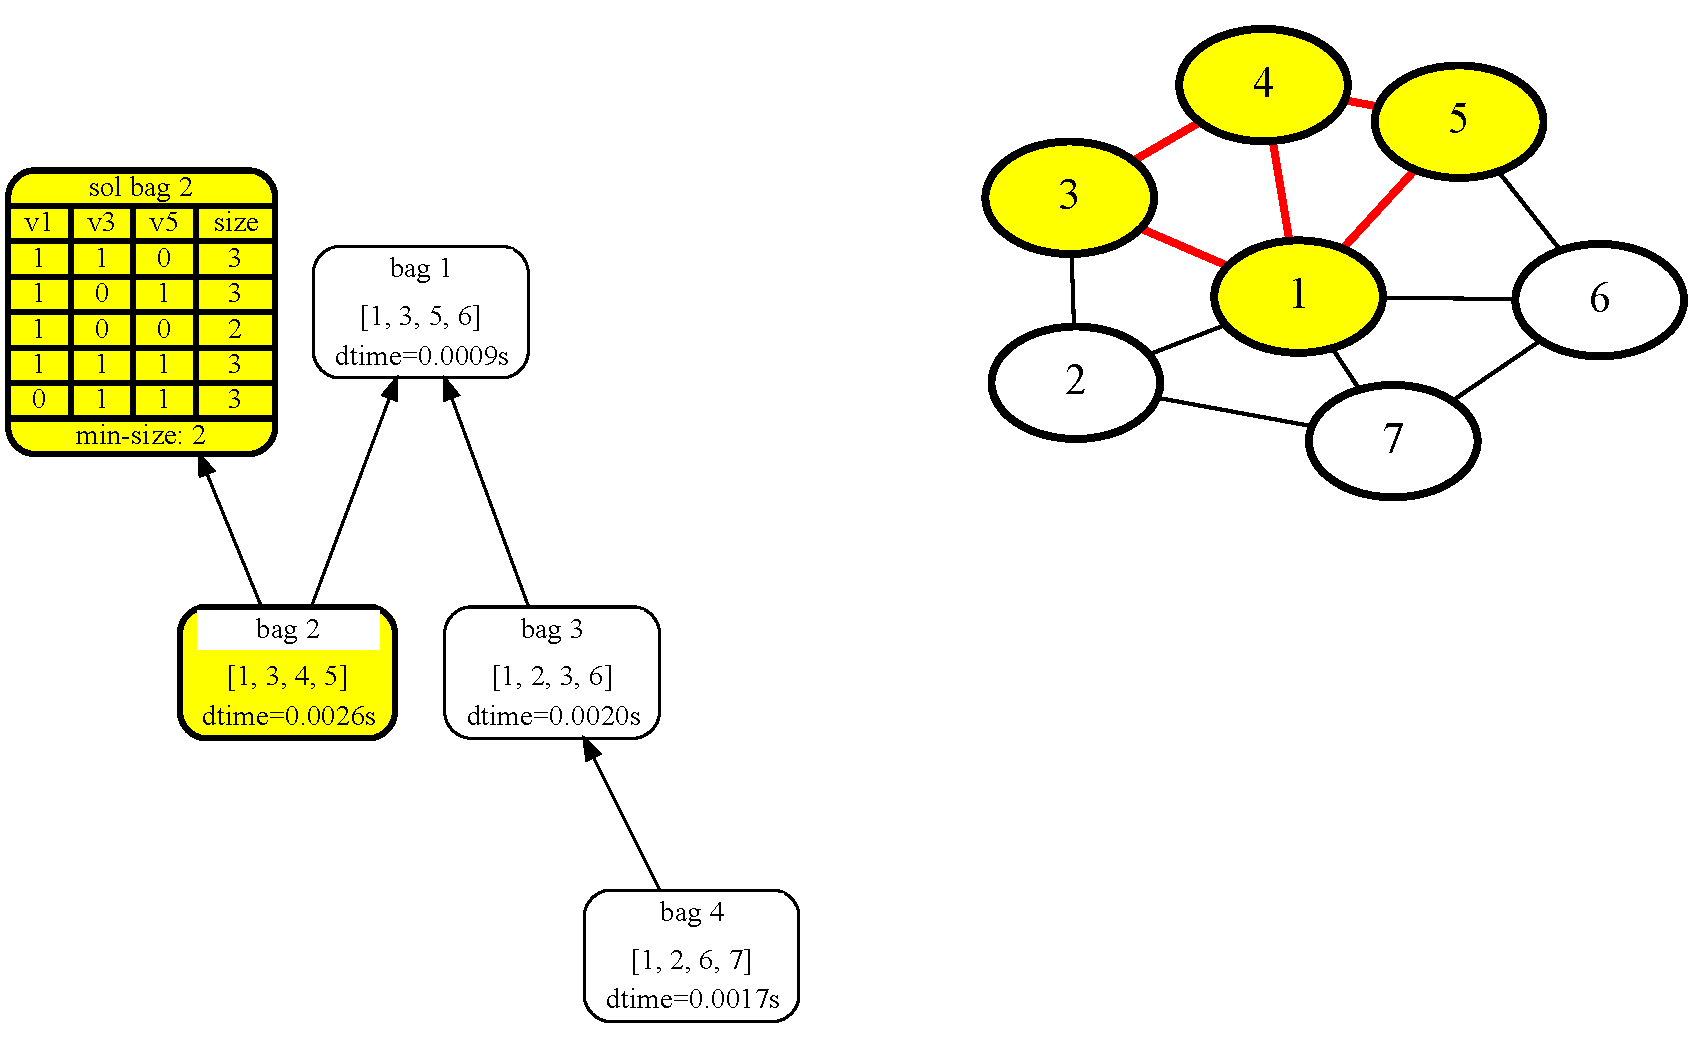
\includegraphics[width=0.9\linewidth,height=0.9\textheight,keepaspectratio]{images/SVGJOIN/default_06sc152.pdf}
	\caption{Joining results from Section \ref{sec:minvc} at step 2. Also shifting the second graphic to $40\%$ height of the first image and scaling with scale2 = 1.5 .}
	\label{fig:joinscaled2}
\end{figure}
\begin{figure}
	\centering
	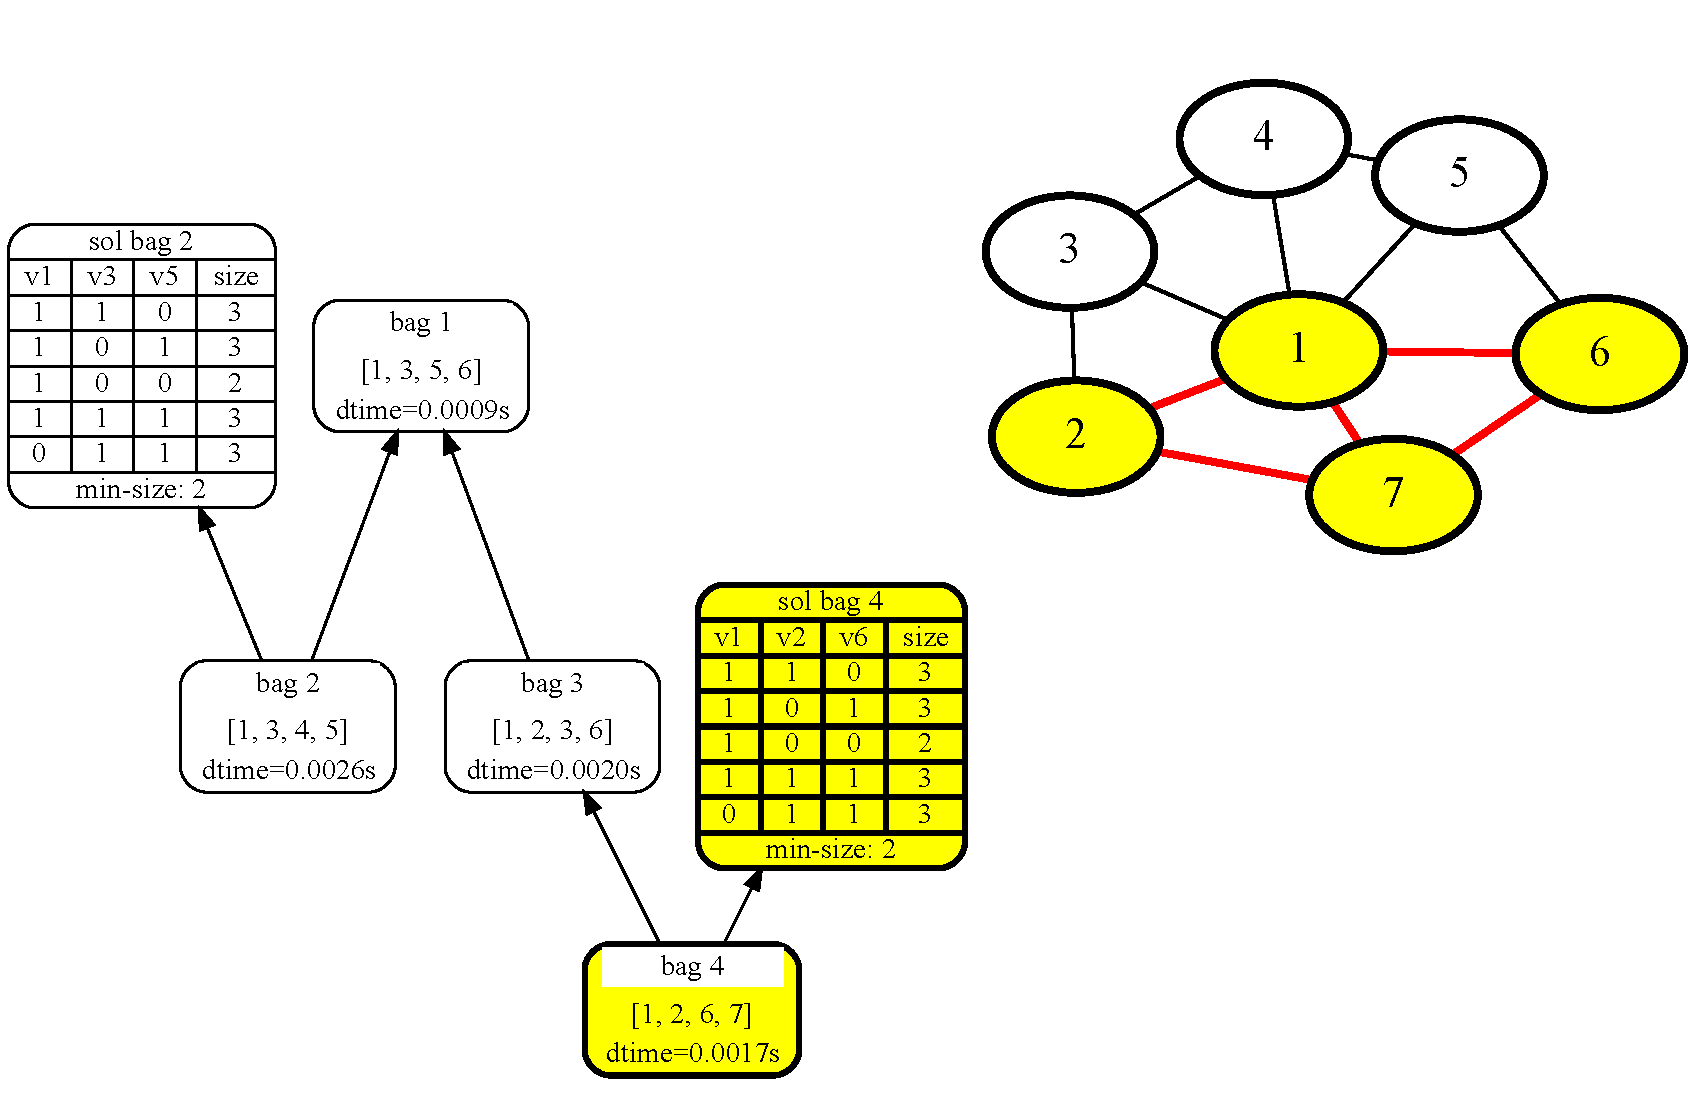
\includegraphics[width=0.9\linewidth,height=0.9\textheight,keepaspectratio]{images/SVGJOIN/default_06sc153.pdf}
	\caption{Joining results from Section \ref{sec:minvc} at step 3. Also shifting the second graphic to $40\%$ height of the first image and scaling with scale2 = 1.5 .}
	\label{fig:joinscaled3}
\end{figure}
\begin{figure}
	\centering
	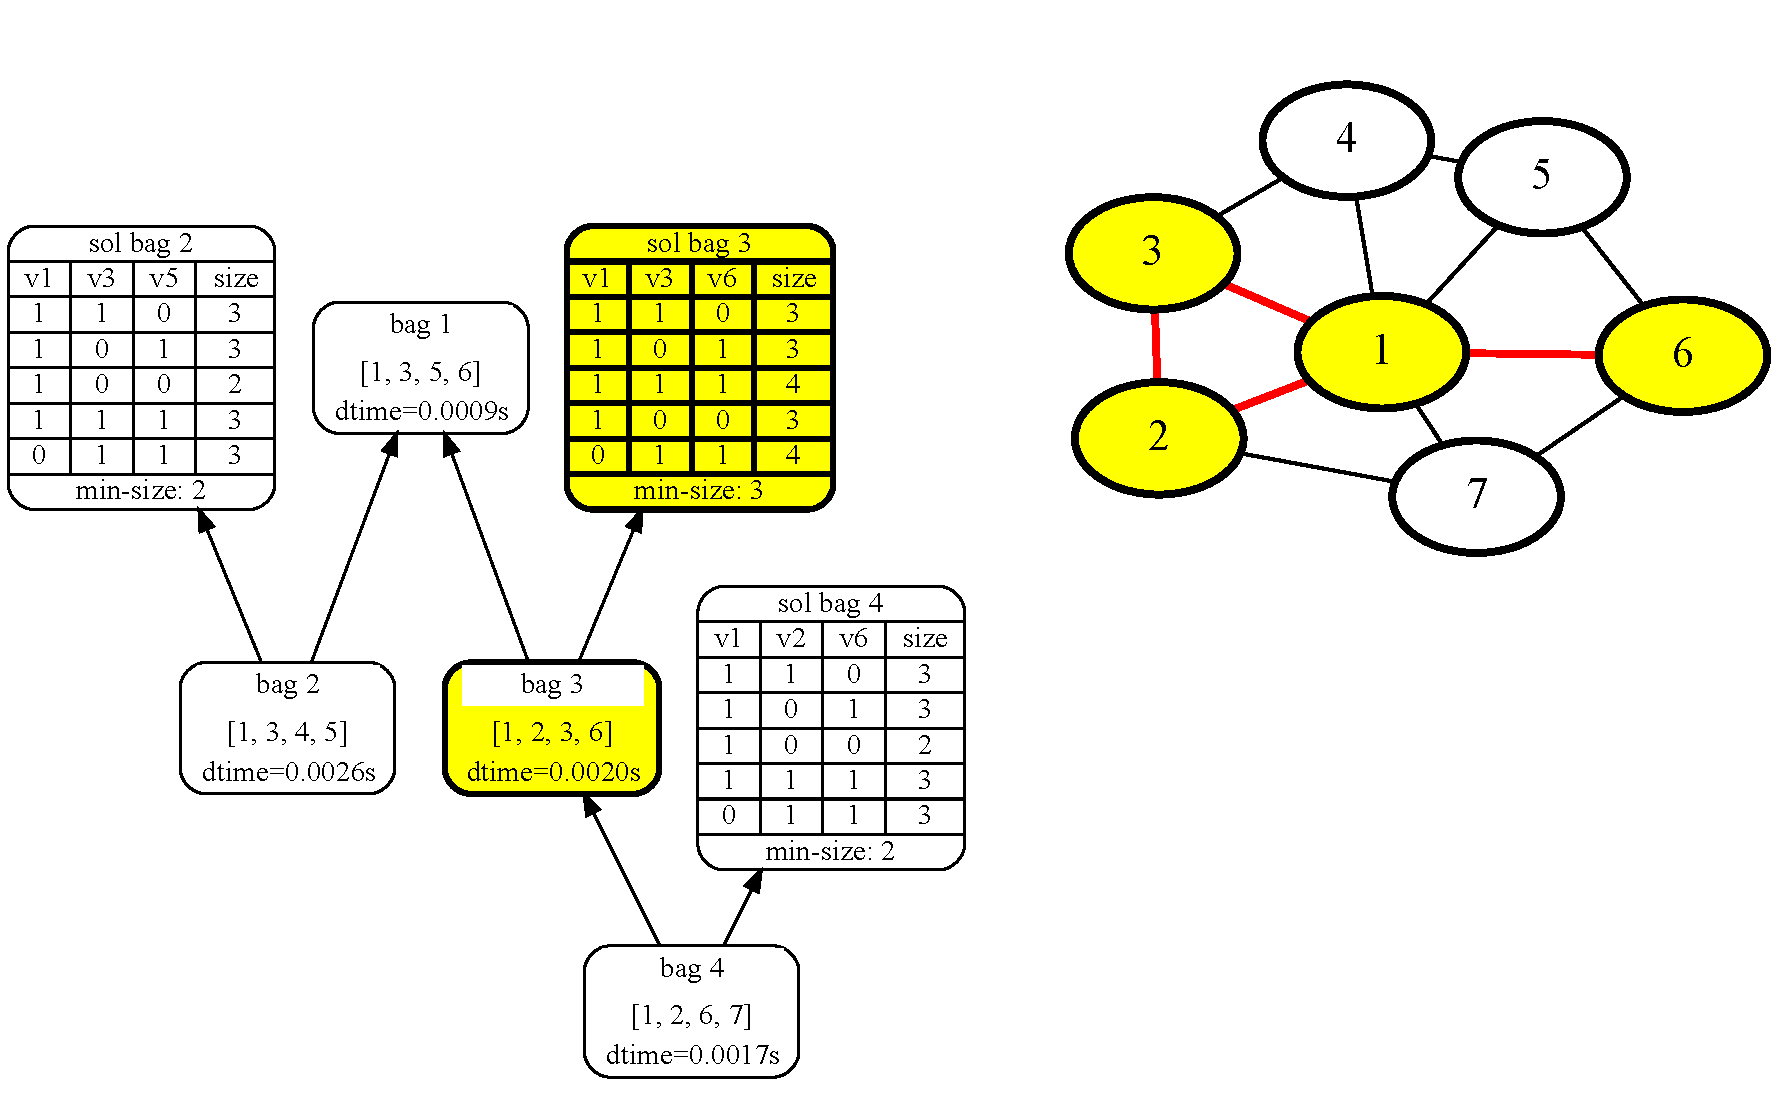
\includegraphics[width=0.9\linewidth,height=0.9\textheight,keepaspectratio]{images/SVGJOIN/default_06sc154.pdf}
	\caption{Joining results from Section \ref{sec:minvc} at step 4. Also shifting the second graphic to $40\%$ height of the first image and scaling with scale2 = 1.5 .}
	\label{fig:joinscaled4}
\end{figure}
\begin{figure}
	\centering
	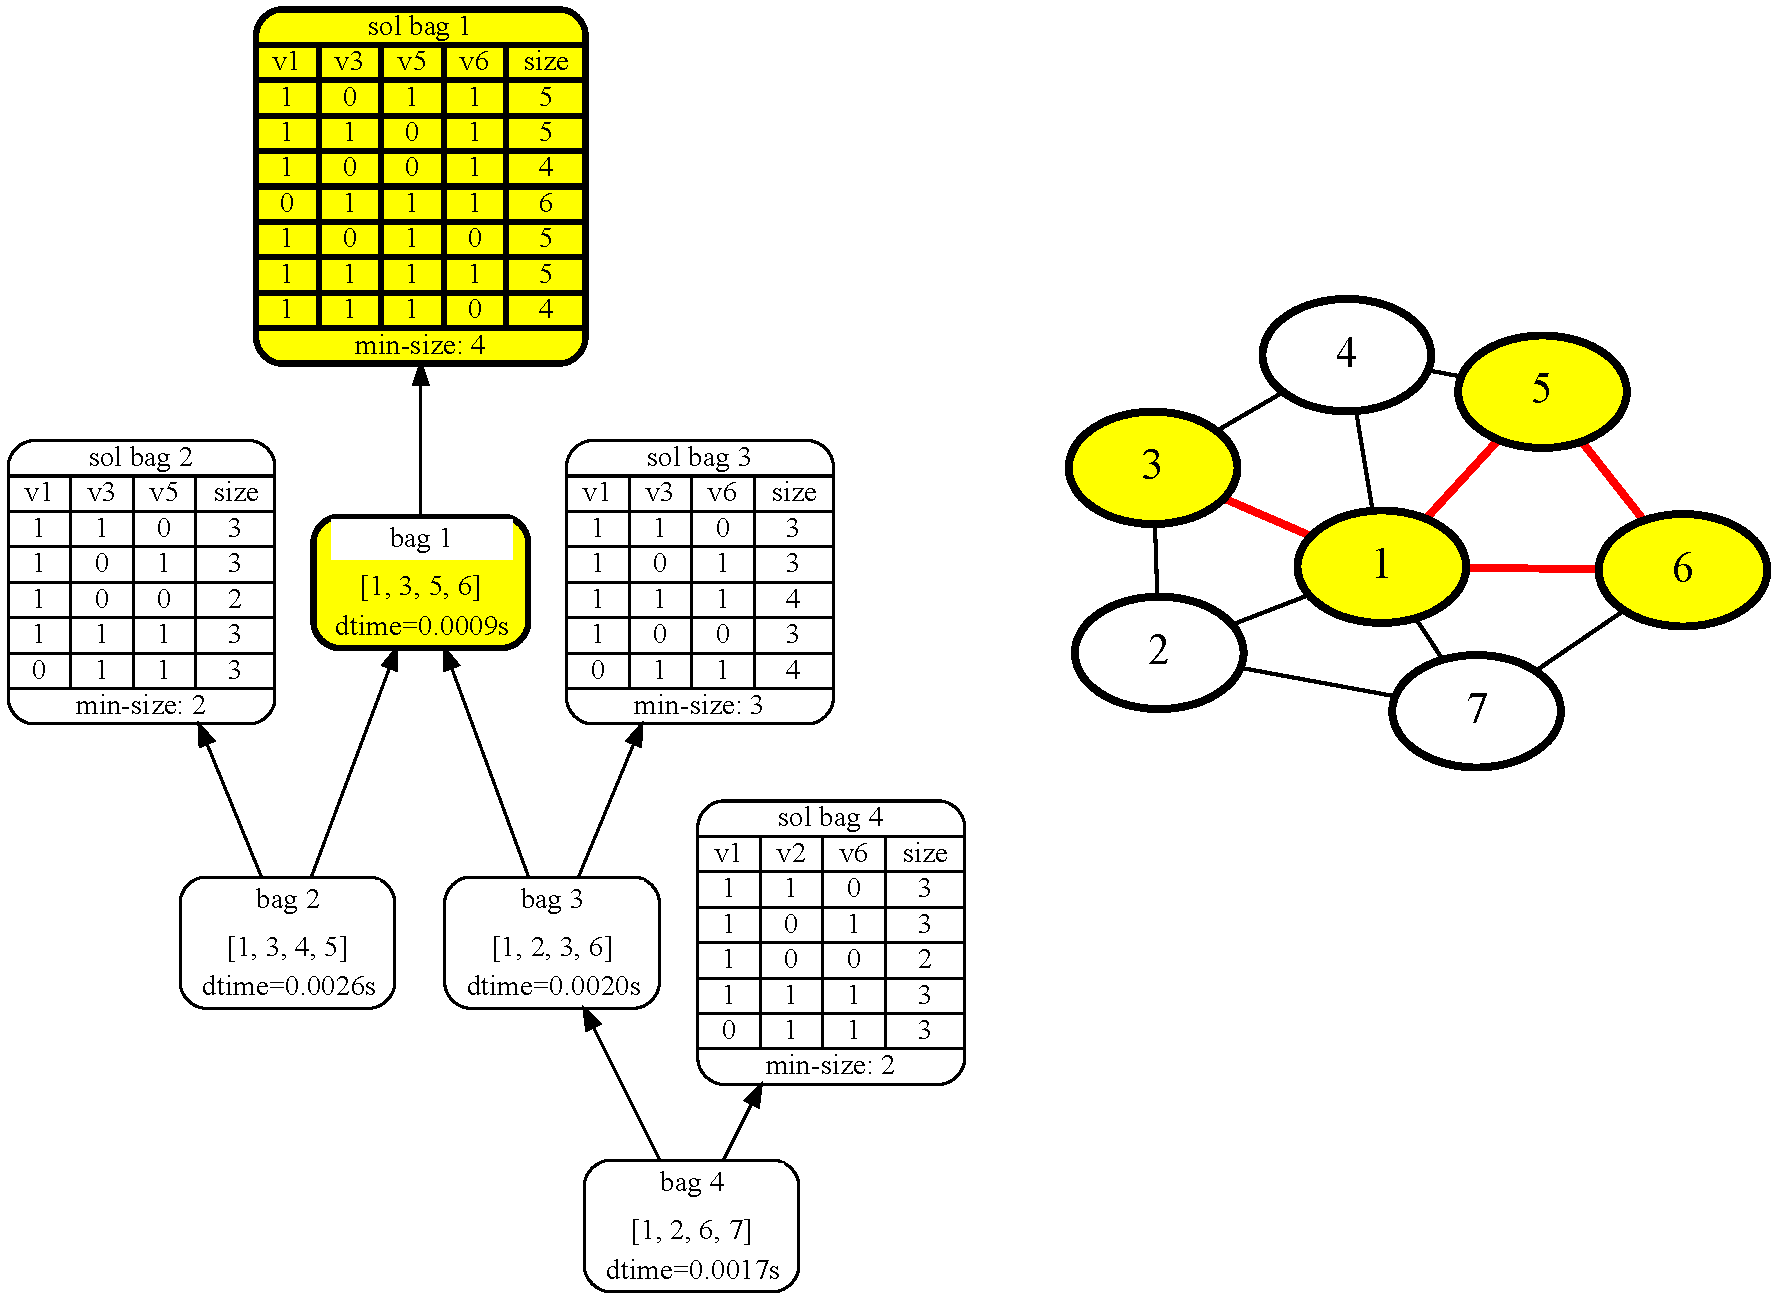
\includegraphics[width=0.9\linewidth,height=0.9\textheight,keepaspectratio]{images/SVGJOIN/default_06sc155.pdf}
	\caption{Joining results from Section \ref{sec:minvc} at step 5. Also shifting the second graphic to $40\%$ height of the first image and scaling with scale2 = 1.5 .}
	\label{fig:joinscaled5}
\end{figure}
%svg_join(['TDStep', 'graph'],
%'Archive/WheelGraph7',
%outname="default_06sc15_rise",
%v_bottom=[1,.85,.7,.55,.4],
%scale2=1.5,
%num_images=5)
\begin{figure}
	\centering
	\includegraphics[width=0.9\linewidth,height=0.9\textheight,keepaspectratio]{images/SVGJOIN/default_06sc15_rise1.pdf}
	\caption{Joining results from Section \ref{sec:minvc} at the first step. Also shifting the second graphic to the bottom edge of the first image and scaling with scale2 = 1.5 .}
	\label{fig:joinscaledrise1}
\end{figure}
\begin{figure}
	\centering
	\includegraphics[width=0.9\linewidth,height=0.9\textheight,keepaspectratio]{images/SVGJOIN/default_06sc15_rise1.pdf}
	\caption{Joining results from Section \ref{sec:minvc} at the second step. Also shifting the second graphic to $15\%$ of the height of the first image and scaling with scale2 = 1.5 .}
	\label{fig:joinscaledrise2}
\end{figure}
\begin{figure}
	\centering
	\includegraphics[width=0.9\linewidth,height=0.9\textheight,keepaspectratio]{images/SVGJOIN/default_06sc15_rise1.pdf}
	\caption{Joining results from Section \ref{sec:minvc} at the third step. Also shifting the second graphic to $30\%$ of the height of the first image and scaling with scale2 = 1.5 .}
	\label{fig:joinscaledrise3}
\end{figure}
\begin{figure}
	\centering
	\includegraphics[width=0.9\linewidth,height=0.9\textheight,keepaspectratio]{images/SVGJOIN/default_06sc15_rise1.pdf}
	\caption{Joining results from Section \ref{sec:minvc} at the fourth step. Also shifting the second graphic to $45\%$ of the height of the first image and scaling with scale2 = 1.5 .}
	\label{fig:joinscaledrise4}
\end{figure}
\begin{figure}
	\centering
	\includegraphics[width=0.9\linewidth,height=0.9\textheight,keepaspectratio]{images/SVGJOIN/default_06sc15_rise1.pdf}
	\caption{Joining results from Section \ref{sec:minvc} at the final step. Also shifting the second graphic to to $60\%$ of the height of the first image and scaling with scale2 = 1.5 .}
	\label{fig:joinscaledrise5}
\end{figure}

%============== Code Snippets ======================================================
\newpage
\section{Code Snippets}

\lstinputlisting[caption={The JSON format used to describe MSOL visualization on tree decompositions}, label={lst:jsonapi}]{includes/JsonAPI.txt}


\begin{lstlisting}[language={Python}, caption={Initializing a Visualization object}, label={lst:visuinit}]
def __init__(self, infile, outfolder) -> None:
"""Copy needed fields from arguments and create VisualizationData.
"""
self.data: VisualizationData = self.inspect_json(infile)
self.outfolder = outfolder

self.tree_dec_digraph = None

def inspect_json(self, infile) -> VisualizationData:
"""Read and preprocess the needed data from the infile into 
VisualizationData.
"""
LOGGER.debug("Reading from: %s", infile)
visudata = read_json(infile)
LOGGER.debug("Found keys: %s", visudata.keys())

try:
_incid = visudata['incidenceGraph']
_general_graph = visudata['generalGraph']
_svg_join = visudata.get('svg_join', None)

incid_data: IncidenceGraphData = None
if _incid:
_incid['edges'] = [[x['id'], x['list']]
for x in _incid['edges']]
incid_data = IncidenceGraphData(**_incid)
visudata.pop('incidenceGraph')
general_graph_data: GeneralGraphData = None
if _general_graph:
general_graph_data = GeneralGraphData(**_general_graph)
visudata.pop('generalGraph')
svg_join_data: SvgJoinData = None
if _svg_join:
svg_join_data = SvgJoinData(**_svg_join)
if 'svg_join' in visudata:
visudata.pop('svg_join')

self.timeline = visudata['tdTimeline']
visudata.pop('tdTimeline')
self.tree_dec = visudata['treeDecJson']
self.bagpre = self.tree_dec['bagpre']
self.joinpre = self.tree_dec.get('joinpre', 'Join %d~%d')
self.solpre = self.tree_dec.get('solpre', 'sol%d')
self.soljoinpre = self.tree_dec.get('soljoinpre', 'solJoin%d~%d')
visudata.pop('treeDecJson')
except KeyError as err:
raise KeyError(f"Key {err} not found in the input Json.")
return VisualizationData(incidence_graph=incid_data,
general_graph=general_graph_data,
svg_join=svg_join_data,
**visudata)

\end{lstlisting}

\begin{lstlisting}[language={Python}, caption={SvgJoinData}, label={lst:svgjoindataclass}]
@dataclass
class SvgJoinData:
"""Class holding different parameters to join the results."""
base_names: Union[str, Iterable[str]]
folder: Optional[str] = None
outname: str = 'combined'
suffix: str = '%d.svg'
preserve_aspectratio: str = 'xMinYMin'
num_images: int = 1
padding: Union[int, Iterable[int]] = 0
scale2: Union[float, Iterable[float]] = 1.0
v_top: Union[None, float, str, 
Iterable[Union[None, float, str]]] = None
v_bottom: Union[None, float, str, 
Iterable[Union[None, float, str]]] = None	
\end{lstlisting}

\begin{lstlisting}[language={Python}, caption={IncidenceGraphData}, label={lst:incidencedata}]
@dataclass
class IncidenceGraphData:
"""Class holding different parameters for the incidence graph."""
	edges: list
	subgraph_name_one: str = 'clauses'
	subgraph_name_two: str = 'variables'
	var_name_one: str = ''
	var_name_two: str = ''
	infer_primal: bool = False
	infer_dual: bool = False
	primal_file: str = 'PrimalGraphStep'
	inc_file: str = 'IncidenceGraphStep'
	dual_file: str = 'DualGraphStep'
	fontsize: int = 16
	penwidth: float = 2.2
	second_shape: str = 'diamond'
	column_distance: float = 0.5
\end{lstlisting}

\begin{lstlisting}[language={Python}, caption={GeneralGraphData}, label={lst:gengraphdata}]
@dataclass
class GeneralGraphData:
"""Class holding different parameters for the general graph."""
edges: list
extra_nodes: Optional[list] = None
graph_name: str = 'graph'
file_basename: str = 'graph'
var_name: str = ''
sort_nodes: bool = False
need_adj_nodes: bool = False
fontsize: int = 20
first_color: str = 'yellow'
first_style: str = 'filled'
second_color: str = 'green'
second_style: str = 'dotted,filled'
\end{lstlisting}

\begin{lstlisting}[language={Python}, caption={Construct\_dpdb\_visu.py}, label={lst:create-json}]
def create_json(problem: int, tw_file=None, intermed_nodes=False):
	"""Create the JSON for the specified problem instance."""
	with connect() as connection:
		# get type of problem
		with connection.cursor() as cur:
				cur.execute("SELECT name,type,num_bags FROM "
				"public.problem WHERE id=%s", (problem,))
				(name, ptype, num_bags) = cur.fetchone()	
		# select the valid constructor for the problem
		constructor: IDpdbVisuConstruct
		
		if ptype == 'Sat':
			constructor = DpdbSatVisu(
				connection, problem, intermed_nodes)
		elif ptype == 'SharpSat':
			constructor = DpdbSharpSatVisu(
				connection, problem, intermed_nodes)
		elif ptype == 'VertexCover':
			constructor = DpdbMinVcVisu(
				connection, problem, intermed_nodes, tw_file)
		
		return constructor.construct()
	return {} 
\end{lstlisting}

\begin{lstlisting}[language={Python}, caption={forward\_iterate\_tdg}, label={lst:forward-iterate}]
def forward_iterate_tdg(self, joinpre, solpre, soljoinpre) -> None:
"""Create the final positions of all nodes with solutions."""
	tdg = self.tree_dec_digraph                 # shorten name
	
	for i, node in enumerate(self.timeline):
		if len(node) > 1:
			# solution to be displayed
			id_inv_bags = node[0]
			if isinstance(id_inv_bags, int):
				last_sol = solpre % id_inv_bags
				tdg.node(last_sol, solution_node(
				*(node[1])), shape='record')	
				tdg.edge(self.bagpre % id_inv_bags, last_sol)
			
			else:    # joined node with 2 bags
				suc = self.timeline[i + 1][0]   # get the joined bags
				
				LOGGER.debug('joining %s to %s ', node[0], suc)
				
				id_inv_bags = tuple(id_inv_bags)
				last_sol = soljoinpre % id_inv_bags
				tdg.node(last_sol, solution_node(
				*(node[1])), shape='record')
				
				tdg.edge(joinpre % id_inv_bags, last_sol)
				# edges
				for child in id_inv_bags:  # basically "remove" current
					tdg.edge(
							self.bagpre % child
							if isinstance(child, int) else joinpre % child,
							self.bagpre % suc
							if isinstance(suc, int) else joinpre % suc,
							style='invis',
							constraint='false')
					tdg.edge(self.bagpre % child if isinstance(child, int)
					         else joinpre % child,
					         joinpre % id_inv_bags)
				tdg.edge(joinpre % id_inv_bags, self.bagpre % suc
					if isinstance(suc, int) else joinpre % suc)
\end{lstlisting}

\begin{lstlisting}[language={Python}, caption={backwards\_iterate\_tdg}, label={lst:backward-iterate}]
def backwards_iterate_tdg(self, joinpre, solpre, soljoinpre,
                          view=False) -> None:
	"""Cut the single steps back and update emphasis acordingly."""
	tdg = self.tree_dec_digraph     # shorten name
	last_sol = ""
	
	for i, node in enumerate(reversed(self.timeline)):
		id_inv_bags = node[0]
		LOGGER.debug("%s: Reverse traversing on %s", i, id_inv_bags)
		
		if i > 0:
			# Delete previous emphasis
			prevhead = self.timeline[len(self.timeline) - i][0]
			bag = (self.bagpre % prevhead if isinstance(prevhead,int) 
					else joinpre % tuple(prevhead))
			base_style(tdg, bag)
			if last_sol:
				style_hide_node(tdg, last_sol)
				style_hide_edge(tdg, bag, last_sol)
				last_sol = ""
		
		if len(node) > 1:
			# solution to be displayed
			if isinstance(id_inv_bags, int):
				last_sol = solpre % id_inv_bags
				emphasise_node(tdg, last_sol)
				tdg.edge(self.bagpre % id_inv_bags, last_sol)
			else:  # joined node with 2 bags
				id_inv_bags = tuple(id_inv_bags)
				last_sol = soljoinpre % id_inv_bags
				emphasise_node(tdg, last_sol)
			
		emphasise_node(tdg,
			self.bagpre % id_inv_bags if isinstance(id_inv_bags, int) else 
			joinpre % id_inv_bags)
		_filename = self.outfolder + self.data.td_file + '%d'
		tdg.render(
			view=view, format='svg', filename=_filename %
			(len(self.timeline) - i))

\end{lstlisting}

\begin{lstlisting}[language={Python}, caption={SvgJoinData}, label={lst:svgjoindata}]
@dataclass
class SvgJoinData:
	"""Class for holding different parameters to join the results."""
	base_names: Union[str, Iterable[str]]
	folder: Optional[str] = None
	outname: str = 'combined'
	suffix: str = '%d.svg'
	preserve_aspectratio: str = 'xMinYMin'
	num_images: int = 1
	padding: Union[int, Iterable[int]] = 0
	scale2: Union[float, Iterable[float]] = 1.0
	v_top: Union[None, float, str, 
	             Iterable[Union[None, float, str]]] = 'top'
	v_bottom: Union[None, float, str, 
	                Iterable[Union[None, float, str]]] = None
\end{lstlisting}

%============== Input Examples ======================================================
\section{More Examples}\label{app:input}

\lstset{numbers=none}

\begin{table}[ht]
	\centering
	\begin{tabular}{|l||c|c|c|c|c|c|c|c|}
		
		\hline
		&$v_{1}$ & $v_{2}$ & $v_{3}$ & $v_{4}$ & $v_{5}$ & $v_{6}$ & $v_{7}$ & $v_{8}$ \\
		\hline 
		1&1 & 1 & 1 & 1 & 1 & 1 & 1 & 1 \\
		2&1 & 1 & 1 & 1 & 1 & 1 & 1 & 0 \\
		3&1 & 1 & 1 & 1 & 0 & 1 & 1 & 1 \\
		4&1 & 1 & 1 & 1 & 0 & 1 & 1 & 0 \\
		5&1 & 1 & 1 & 0 & 1 & 1 & 1 & 0 \\
		6&1 & 1 & 1 & 0 & 1 & 0 & 1 & 0 \\
		7&1 & 1 & 1 & 0 & 0 & 1 & 1 & 0 \\
		8&1 & 1 & 1 & 0 & 0 & 0 & 1 & 0 \\
		9&1 & 1 & 0 & 1 & 1 & 1 & 1 & 0 \\
		10&1 & 1 & 0 & 1 & 0 & 1 & 1 & 0 \\
		11&1 & 1 & 0 & 0 & 1 & 1 & 1 & 0 \\
		12&1 & 1 & 0 & 0 & 1 & 0 & 1 & 0 \\
		13&1 & 1 & 0 & 0 & 0 & 1 & 1 & 0 \\
		14&1 & 1 & 0 & 0 & 0 & 0 & 1 & 0 \\
		15&1 & 0 & 1 & 0 & 0 & 0 & 1 & 0 \\
		16&0 & 1 & 1 & 1 & 0 & 1 & 1 & 1 \\
		17&0 & 1 & 1 & 1 & 0 & 1 & 1 & 0 \\
		18&0 & 1 & 1 & 0 & 0 & 1 & 1 & 0 \\
		19&0 & 1 & 1 & 0 & 0 & 1 & 0 & 0 \\
		20&0 & 1 & 0 & 1 & 0 & 1 & 1 & 0 \\
		21&0 & 1 & 0 & 0 & 0 & 1 & 1 & 0 \\
		22&0 & 1 & 0 & 0 & 0 & 1 & 0 & 0 \\
		\hline
	\end{tabular}
\caption{The satisfying assignments for the formula from Example~\ref{ex:example41}.}
\label{tab:ex41tabx}
\end{table}

\begin{lstlisting}[caption={CNF clauses from example 4.1 in \cite{DiplomarbeitZisser} page 27}, label={lst:clausesDA41}]
p cnf 8 10
1 4 6 0
1 -5 0
-1 7 0
2 3 0
2 5 0
2 -6 0
3 -8 0
4 -8 0
-4 6 0
-4 7 0
\end{lstlisting}
\begin{lstlisting}[caption={CNF clauses from random example with 12 units},label={lst:example18-24}]
p cnf 18 24
-1 0
-2 0
-3 0
-4 0
-5 0
-6 0
-7 0
-8 0
-9 0
-10 0
-11 0
-12 0
-13 -14 -15 0
-13 -14 16 0
-13 -15 -16 -18 0
-13 -15 -17 0
13 14 16 -17 18 0
13 15 -16 -18 0
-14 -15 16 17 0
-14 15 -17 18 0
-14 15 17 -18 0
-15 -16 -17 18 0
15 -16 -17 -18 0
15 16 17 -18 0
\end{lstlisting}
\lstinputlisting[caption={Edges for example \ref{fig:wheelgraph}}, label={lst:wheelgraph}]{images/WheelGraph7/wheelgraph7.tw}
\lstinputlisting[caption={Tree decomposition for example \ref{fig:wheelgraph}}, label={lst:wheelgraphtd}]{images/WheelGraph7/wheelgraph7.td}
\lstinputlisting[caption={DOT source for visualization of example 4.1}, label={lst:g41digraphdot}]{includes/g41digraphdot}
\lstinputlisting[caption={stdout of program gpusat with call \textit{./gpusat -f ../examples/test\_da4\_1.cnf -v -p -d ../examples/td4p1.txt  -g ../examples/graphfileda41.txt -{}-visufile ../examples/visufileda41.json}}, label={lst:outputGpusat}]{includes/outputGpusat.txt}

%==============================================================================
%============== BIBLIOGRAPHY ==================================================
%==============================================================================
\newpage
\printbibliography
%\bibliography{bibtex}{}
%\bibliographystyle{ieeetr}
\end{document}
